
\documentclass[prodmode,acmtochi]{acmsmall}

%{{{ initial definitions
\usepackage{url}
\usepackage{graphics}
\usepackage{color}
\usepackage[usenames,dvipsnames]{xcolor}
\usepackage{datetime}

% Colours
\definecolor{Orange}{rgb}{1,0.5,0}
\definecolor{Shadow}{rgb}{100,100,100}
\definecolor{Shadowy}{rgb}{0.2,0.2,0.2}
\definecolor{Purple}{RGB}{186,85,211}
\definecolor{Blue}{RGB}{135,206,250}
\definecolor{LightBlue}{RGB}{30,144,255}


%\usepackage{float}
%\usepackage{trivfloat}

%\newfloat{tablik}{thb}{lop}
%\floatname{tablik}{Table}
%\trivfloat{tablik}
\usepackage[font=small,labelfont=bf]{caption}
\renewcommand{\thetable}{\arabic{table}}

% Commands
\newcommand{\comment}[1]{}
\newcommand{\killedForSpace}[1]{}
\newcommand{\todo}[1]{\textrm{\textrm{\textcolor{LightBlue}{[[#1]]}}}}
\newcommand{\forGer}[1]{\textrm{\textbf{\textcolor{LightBlue}{[[#1]]}}}}
\newcommand{\Geraldine}[1]{\textrm{\textbf{\textcolor{Orange}{[[#1]]}}}}
%\newcommand{\Geraldine}[1]{}
\newcommand{\GeraldineFIX}[1]{}



%%%%%%%%%%%%%%%%%%%%%%%%%%%%%%%%%%%%%%%%%%%%%%%%%%%%%
%%%%%%%%%%% GERALDINE COMMENTS -- ON/OFF %%%%%%%%%%%%
%%%%%%%%%%%%%%%%%%%%%%%%%%%%%%%%%%%%%%%%%%%%%%%%%%%%%

\newcommand{\GeraldineFIXNEW}[1]{}
%\newcommand{\GeraldineFIXNEW}[1]{\textcolor{gray}{#1}}

%%%%%%%%%%%%%%%%%%%%%%%%%%%%%%%%%%%%%%%%%%%%%%%%%%%%%
%%%%%%%%%%%%%%%%%%%%%%%%%%%%%%%%%%%%%%%%%%%%%%%%%%%%%
%%%%%%%%%%%%%%%%%%%%%%%%%%%%%%%%%%%%%%%%%%%%%%%%%%%%%




\newcommand{\GeraldineTODO}[1]{}
%\newcommand{\GeraldineTODONEW}[1]{\textcolor{gray}{#1}}
\newcommand{\TODO}[1]{\textrm{\textbf{\textcolor{Red}{[[#1]]}}}}
\newcommand{\GeraldineDIS}[1]{}
\newcommand{\todolater}[1]{}
\newcommand{\remove}[1]{}
\newcommand{\rephrase}[1]{\textrm{\textrm{\textcolor{gray}{#1}}}}
\newcommand{\revision}[1]{#1}
\newcommand{\qq}[2]{\textrm{\textit{``#2''}}{ [#1]}}
\newcommand{\inqq}[1]{\textrm{\textit{``#1''}}}
\newcommand{\qqq}[1]{\begin{quotation} \emph{``#1''} \end{quotation}}
\newcommand{\ger}[2]{\textcolor{LightBlue}{#1} -- \textcolor{Purple}{#2}}
\newcommand{\citet}[1]{\cite{#1}}


% References library 
%\usepackage[sort]{natbib}


%\emergencystretch=1em

%\pagenumbering{arabic}  % arabic page numbers for submission.  remove this line to eliminate page numbers for the camera ready copy

\begin{document}

% to make various latex processors do the right thing with page size
%\special{papersize=8.5in,11in}
%\setlength{\paperheight}{11in}
%\setlength{\paperwidth}{8.5in}
%\setlength{\pdfpageheight}{\paperheight}
%\setlength{\pdfpagewidth}{\paperwidth}

%\renewcommand{\harvardurl}{URL: \url}

% use this command to override the default acm copyright statement
% (e.g. for preprints). remove for camera ready copy.
%\toappear{submitted for review to chi 2009.}

\title{Teaching and Developing Social and Emotional Skills \\ with Technology} 
%\numberofauthors{1}
% blinded authors
\author{PETR SLOV\'{A}K %, Wolfgang Reitberger, Geraldine Fitzpatrick
     \affil{Vienna University of Technology}
 GERALDINE FITZPATRICK \affil{Vienna University of Technology}
Version from \affil{ \today, \currenttime }
	}
        
%\abstract{ This is a desperate abstract of an abstract. 

%}
\iffalse

\author{
  \alignauthor ~\\
      \affaddr{~}\\
      \affaddr{~}\\
      \affaddr{~}
}
\fi     

\maketitle
%}}}

% {{{  --- Abstract 
\section*{Abstract} 
Supporting social interactions is a long term focus for HCI and CSCW. However, understanding how social and emotional skills are learned, and how this process can be supported by technology, is an important but underresearched area so far. 
% 
This paper reviews the approaches to social and emotions skills learning (SEL) outside of HCI, where a large number of evidence-based programs is widely deployed. However, very little technology gets used in these programs, despite its potential to enhance and complement the existing approaches.  
%
%Primary aim of this paper is to provide a foundation and set an agenda for future research on the design of technology that would support, and help teach, social and emotional skills. 
% with specific focus on the long history and experience around SEL in education,
%
The primary aim of this paper is to provide a foundation and set an agenda
for future research on the design of technology that would support, and help
teach, social and emotional skills. To this end, we review the literature on social and emotional learning courses with specific focus on the long history and experience around SEL in education. We identify similarities among the curricula used there, and the shared challenges to successful learning that might be addressed by technology. We then link these to HCI research and the potential for both fields to be mutually enriched. 

Our key argument is that much existing HCI work could be used in support of social and emotional skills learning (SEL) in education---and possibly other domains---but that the topic has been under-researched so far within HCI. We argue how such technology could fundamentally extend and enhance the possibilities available to social skills learning, such as supporting the embedding of skills in class into everyday situations, promoting reflection, and providing additional environments for practice. We also outline how the focus on SEL would bring the novel opportunities and challenges for HCI, as well as a structure to guide and support HCI in this emerging research direction. 

%\GeraldineFIX{G: Overall comments/notes:  \\ 1. US or UK\ conventions? eg UK:\  double quotes for text directly taken from texts, single quotes for phrases etc (reverse US); enroll US  but enrol outside of US; practice - noun, practise - verb in UK but practice used as noun and verb in US; etc \\ 2. how multiple authors are referenced in text eg p9 Arthur, Winfred et al OR Bono et al? \\ 3. Does autism/social disability need to be included as one of the domains since so many of the HCI-related examples are drawn from autism [discussed - to add a sentence or so to therapy section]\\ 4. think it would be really beneficial to have a table or figure summarising eg list of topics and/or methods across curricula? [OK\ have discussed this is hard/impossible!]\\ 5. Figure numbering is all out of whack [maybe just in my printed version though... seems might be ok in this version       }
   

%\todo{Draw out the key structures here already?} %In particular, we draw out learning principles (feedback, practice, embedding into everyday life, and engagment) shared by social and emotional skills learning curricula across domains 
% }}}


% {{{ SECTION: Introduction
\section{Introduction}

Social and emotional skills refer to a variety of skills that are crucial for our everyday life and healthy development \cite{Weare2011,Adi2007a,Damon2006}, including skills such as those related to emotional intelligence, interpersonal and communication skills, but also skills such as mindfulness, self-control and empathy.
%
Understanding how such social and emotional skills are learned, and how this learning process can be supported by technology, is an emerging area of research within HCI. 

The growing interest in this topic is manifested by recent work around social skills learning in autism \cite{Kientz2013}, computerised Cognitive Behavioural Therapy \cite{Coyle2007}, as well as a number of individual systems aiming to affect particular social behaviour such as discussion dominance or rapport \cite{Balaam2011,Kim2008}. Despite this impressive growth over recent years, the existing body of work is still in early stages, with  with two important limitations: 
	First, most of the research so far is limited in scope, focusing on specific disadvantaged populations, especially the support for people with autism. This leaves out other populations and settings where social and emotional skills learning is crucial. 
	Second, the majority of the existing work has provided only limited evidence to show the effect of training in real-world situations over a longer term (cf. \cite[p. 108-109]{Kientz2013} for a summary of autism related research), with projects often focusing on exploratory short-term pilot deployments and preliminary evaluations only. 

In contrast, a number of interventions and courses have been developed outside of HCI to specifically support social and emotional skill learning (SEL) in everyday settings, and for a wide range of users across many diverse domains such as school education, clinical settings, and leadership \cite{Greenberg2010,Stepien2006,Barth2011,Carey2011,Bono2009}. In particular, \emph{SEL in school education} draws on 20+ years of history in teaching social and emotional skills through carefully designed, evidence-based programs that support a broad set of social and emotional skills needed for adult life. Moreover, the wide scale deployments of these programs build on established methodologies to evaluate the effect of such curricula on learners' behaviour, with data showing that such skills are teachable and that the programs can lead to measurable improvements \cite{Durlak2011,Weare2011}. However to date, very little if any technology gets used in the current curricula. 

The contribution of this paper is to review the SEL curricula used in education and, through this, to point to the unique opportunity for cooperation and mutual enrichment of SEL and HCI research, drawing on the overlap of complementary interests and knowledge around social and emotional learning. 
%
% <HCI gives SEL>
From the HCI side, our review of SEL curricula highlights a number of challenges faced by SEL practitioners---such as the lack of support for students' learning outside of SEL training lessons and in everyday situations---that could be addressed by technology. We argue that although much of existing HCI work has not, so far, been connected to social skills training, it is actually highly relevant and could be further adapted and targeted to support existing SEL curricula.  %Moreover, these SEL challenges also raise opportunities for new HCI research to explore if and how we can design technologies specifically targeted to support social and emotional learning more generally. 
%
% <SEL gives HCI> 
From the SEL side, we show how the knowledge base and existing curricula structure of SEL could support and guide HCI research around social and emotional learning. For example, SEL in education is likely to prove a good test-bed for cutting edge HCI systems. SEL curricula offer a wide range of well defined skills to be supported, controlled real-life context to deploy in, various levels of pre-existing scaffolding to drive learning, and well-established evaluations methods to assess the effects of interventions -- all aspects that HCI designers can benefit from when developing, deploying, and evaluating novel technology. Focus on SEL challenges can help HCI researchers to decide on which skills, and in which order, should we aim to support through technology in the first place; as well as how best to do so. 
%
Overall, this paper aims to contribute towards defining a systematic programme of research for HCI in support of social and emotional learning through technology. 

The remainder of this paper is divided into seven sections.  We first focus on SEL in schools as the exemplary domain (Section~\ref{sec:SEL}), given its longest history of both academic research and practical applications, and the  widest range of life skills. The following three sections link the SEL literature in education to particular examples of, and opportunities for, HCI research. We first identify the key challenges across the existing social and emotional skill curricula from an HCI perspective and point to initial HCI work suggesting how these could be addressed by technology (Section~\ref{sec:HCIsupport}). We continue by outlining how such a focus on SEL would raise interesting research opportunities for HCI (Section~\ref{sec:HCIopportunities}) and suggest the next steps HCI community could make to engage with supporting SEL learning (Section~\ref{sec:HCInextsteps}). 
Section~\ref{sec:linkDomains} steps away from SEL in education to highlight several other domains where learning of social and emotional skills is crucial (therapeutic, medical, workplace, and everyday life settings). We provide a brief overview of SEL methods and topics within each domain to inspire and guide future work, before summarising and concluding the paper (Section~\ref{sec:conclusion}).  




%First, SEL programs face the need to better support 'embedding' of the social and emotional skills learned during sessions into everyday life of the students. While the existing approaches, such as homeworks, essays etc., go only so far, drawing on the recent advances in mobile, ubiquitous and sensing technology could make a big difference.

%Second, existing curricula bring structure and a list of activities that could be supported by digital technology -- allowing tech to be specialised for a specific role, and fit into existing practices, rather than having to take care of all. A similar situation in the related areas of autism or CBT, where the fact that technology support and enhances existing practices helps guide research and pose clear research questions. 
% }}}

\iffalse
% {{{ SECTION -  Introduction
\section{Introduction -- old}
 
 Social and emotional skills refer to a range of skills that are crucial for our everyday life and healthy development \cite{Weare2011,Adi2007a,Damon2006}.We define the term broadly here to include skills such as those related to emotional intelligence, interpersonal and communication skills, and also skills such as mindfulness, self-control and empathy. 

The importance of such skills for personal competence and well-being is acknowledged both in research and industry \cite{Durlak2011,Greenberg2010,Stepien2006,Barth2011,Carey2011,Bono2009}. Social and emotional skills are particularly valued in diverse domains such as education (from kindergarten to university education), leadership, social work, psychotherapy, and medical/clinical settings. 

%\todo{This is particularly important for schools as ... societal blah from Cohen2001 and others? around how many students have obvious SEL problems and how teaching could help with these.}
        %
%       For example, these can be \emph{education} (across all age ranges, i.e., from kindergarden to university education), \emph{workplace related} (ranging from specific soft-skills courses for employees and business students (such as communication, presentation and conflict management skills) to more general approaches such as executive coaching for managers), \emph{medical personell} (communication skills, empathy for students and practitioners), \emph{therapy} related (psychotherapists training and practice, counselling), \emph{mindfulness and calming technology} (novel area, related to stressful environment and problems with work-life balance, with technology partially to blame -- see e.g., workshop or the interactions paper; approaches to support more sustainable lifestyle). 

An increasing number of interventions and courses are designed specifically to support social and emotional skill learning (SEL) in these areas, substantiated by a large body of peer-reviewed, scientific literature showing that \emph{such skills are teachable} and \emph{interventions can lead to measurable improvements}. 
%
However, very little if any digital technology gets used in the current curricula. This opens opportunities to explore if and how HCI could support social and emotional learning within this domain, especially in combination with the growing interest on research relevant to teaching or influencing social and emotional skills within HCI community\footnote{Research on using technology to support learning in more classical academic subjects such as mathematics, programming, physics or languages  has a longer history within HCI, including a number of well-established journals, e.g., Computers \& Education. As further discussed in Section 2.3, while we reference selected articles, we do not review this literature in detail as it is mostly focused on declarative, content-based learning, rather than procedural, skills-based learning that is crucial for SEL.}. 
%       There is growing interest in similar topics within HCI,   %Moreover, as only very little technology support is used in the interventions and curricula in practice at the moment, it leaves many opportunities (and challenges) for improvement. 
For example, a large body of work has recently focused on autism (see, e.g.,  \cite{Kientz2013} for a detailed review), and on using technology to enhance or facilitate psychotherapy \cite{Coyle2011,Matthews2011,DeSa2010,Hancock2010}. Prior literature also includes smaller scale systems aiming to  affect particular social behaviour such as discussion dominance, or rapport e.g., \cite{Narumi2009,Piper2006,Balaam2011,Kim2008,McAtamney2006,Schroyen2008,Kim2008a,Toups2007,Kreitmayer2012,Daily2010,Munson2010}. 
%
%
Wider interest in emotional and social skills within HCI is also exemplified for example by CHI workshops on 'Interaction Design and Emotional Wellbeing' (CHI'12), 'Patient-Clinician Communication' (CHI'13) or 'Enabling Empathy in Health care' (CHI'14); as well as a Special Interest Group (SIG) on Work-life Balance. 

Given this, it is timely then that the potential of technology to support social and emotional skills training and development is explored in a more thorough way.
This paper reviews mainly literature in school education, where various forms of social and emotional skills teaching are key, and connects these to existing work in HCI. 
%
In doing so, we identify shared aspects and differences across curricula, using these to draw out structure for future work and show potential for mutual enrichment of SEL and HCI research fields. 
%
The overall aim is to take the first steps towards a more principled approach
to defining a systematic programme of research for HCI in support of SEL. 

In particular, we argue that there are core methods and challenges to teaching social and emotional skills which are shared across individual SEL curricula; and that these raise new opportunities for HCI research to explore if and how state of the art technologies can help address the challenges in SEL, as well as help support SEL more generally.
%
%We outline both the methods and topics that social and emotional skills curricula use, drawing out key aspects where HCI involvement would be useful.
%
Moreover, we argue that although much of existing HCI work was not, so far, connected to social skills training, it is actually highly relevant and could be beneficial for augmenting existing curricula.
%
We then point to particular opportunities for further research into this topic, outlining the potential of such mutually enriching connections in more detail. 



The remainder of this paper is divided into seven sections.  We first focus on SEL in schools  as an exemplary domain (Section~\ref{sec:SEL}), given it has the longest history of both academic research and practical applications, and addresses  the widest range of life skills. The following three sections link the SEL literature in education to particular examples of, and opportunities for, HCI research. We first  identify the key challenges across the existing social and emotional skill curricula from an HCI perspective and point to initial HCI work suggesting how these could be addressed by technology (Section~\ref{sec:HCIsupport}). We continue by outlining how such focus on SEL would raise interesting research opportunities for HCI (Section~\ref{sec:HCIopportunities}) and suggest the next steps HCI community could make to engage with supporting SEL learning (Section~\ref{sec:HCInextsteps}). 
We then step away from SEL in education for a moment to outline other domains where learning of social and emotional skills is crucial (workplace, medical, psychotherapeutic, and everyday life settings), providing a brief overview of SEL methods and topics within each to inspire and guide future work (Section~\ref{sec:linkDomains}). Finally, Section~\ref{sec:conclusions} \rephrase{summarises and wraps up the paper.}  
\todolater{Downplay the direct applicability to SEL --> existing work albeit in other topics, makes it plausible that it could support SEL.}

\todolater{Results overview}

\iffalse

\paragraph{Results overview}
Our review shows that although the interpretation and context of specific taught skills  differs across the educational curricula, there are substantial similarities in the methods used and the challenges that face curricula designers; and that these could be supported by technology
%
We also outline how all interventions will need to build on the emphasis that social and emotional skills interventions place on experiential learning. This then brings the related aspects of the need for substantial \emph{practice} and \emph{cueing reflection??}, the key importance of the \emph{transfer of learned skills} from facilitated sessions into everyday real world settings and the \emph{need to motivate and engage} learners.

We use these learning principles as an initial structure to guide designers and researchers in thinking about ways to support SEL in each of the diverse domains; and show how this fits well with, and could easily benefit from, existing HCI work on ubiquitous computing, social signals processing, behavioural change, and ``into the wild'' research (see Table~\ref{fig:HCIsummary} on page~\pageref{fig:HCIsummary}). 
%connecting it with opportunities for, and existing work in, HCI research. 
%
%We also outline specific areas where HCI involvement could be particularly helpful . 

\paragraph{Multi-level paper structure}
The text is structured to allow for several ways in which readers can approach the paper. We provide a detailed overview of the SEL literature as well as the examples of potential technology support. This is meant to serve as an initial 'guidepost' for readers interested in learning more about the specific sub-topics, and as an argument base for the interpretations we make, but could be deemed as too detailed for others. For this reason, we keep all such detail in the third level subsections (e.g., 2.4.X or all third level subsections in section \ref{sec:HCIsupport}) and the paper can be read also by skipping these entirely. Similarly, readers interested only in the key implications for HCI can jump directly to Sections~\ref{sec:summary} to \ref{sec:agenda}, leaving out the review of SEL literature. 


\fi


%This is meant to serve as an initial 'guidepost' for readers interested in learning more about those specific topics\footnote{\dots and as an argument base for the interpretations we make.},  but could be deemed as too detailed for others. For this reason, we attempted to keep all such detail in the third level subsections (e.g., 2.4.X or all third level subsections in section \ref{sec:HCIsupport}), and the paper can be read also by skipping these entirely. 

\iffalse
\begin{table}
\centering
	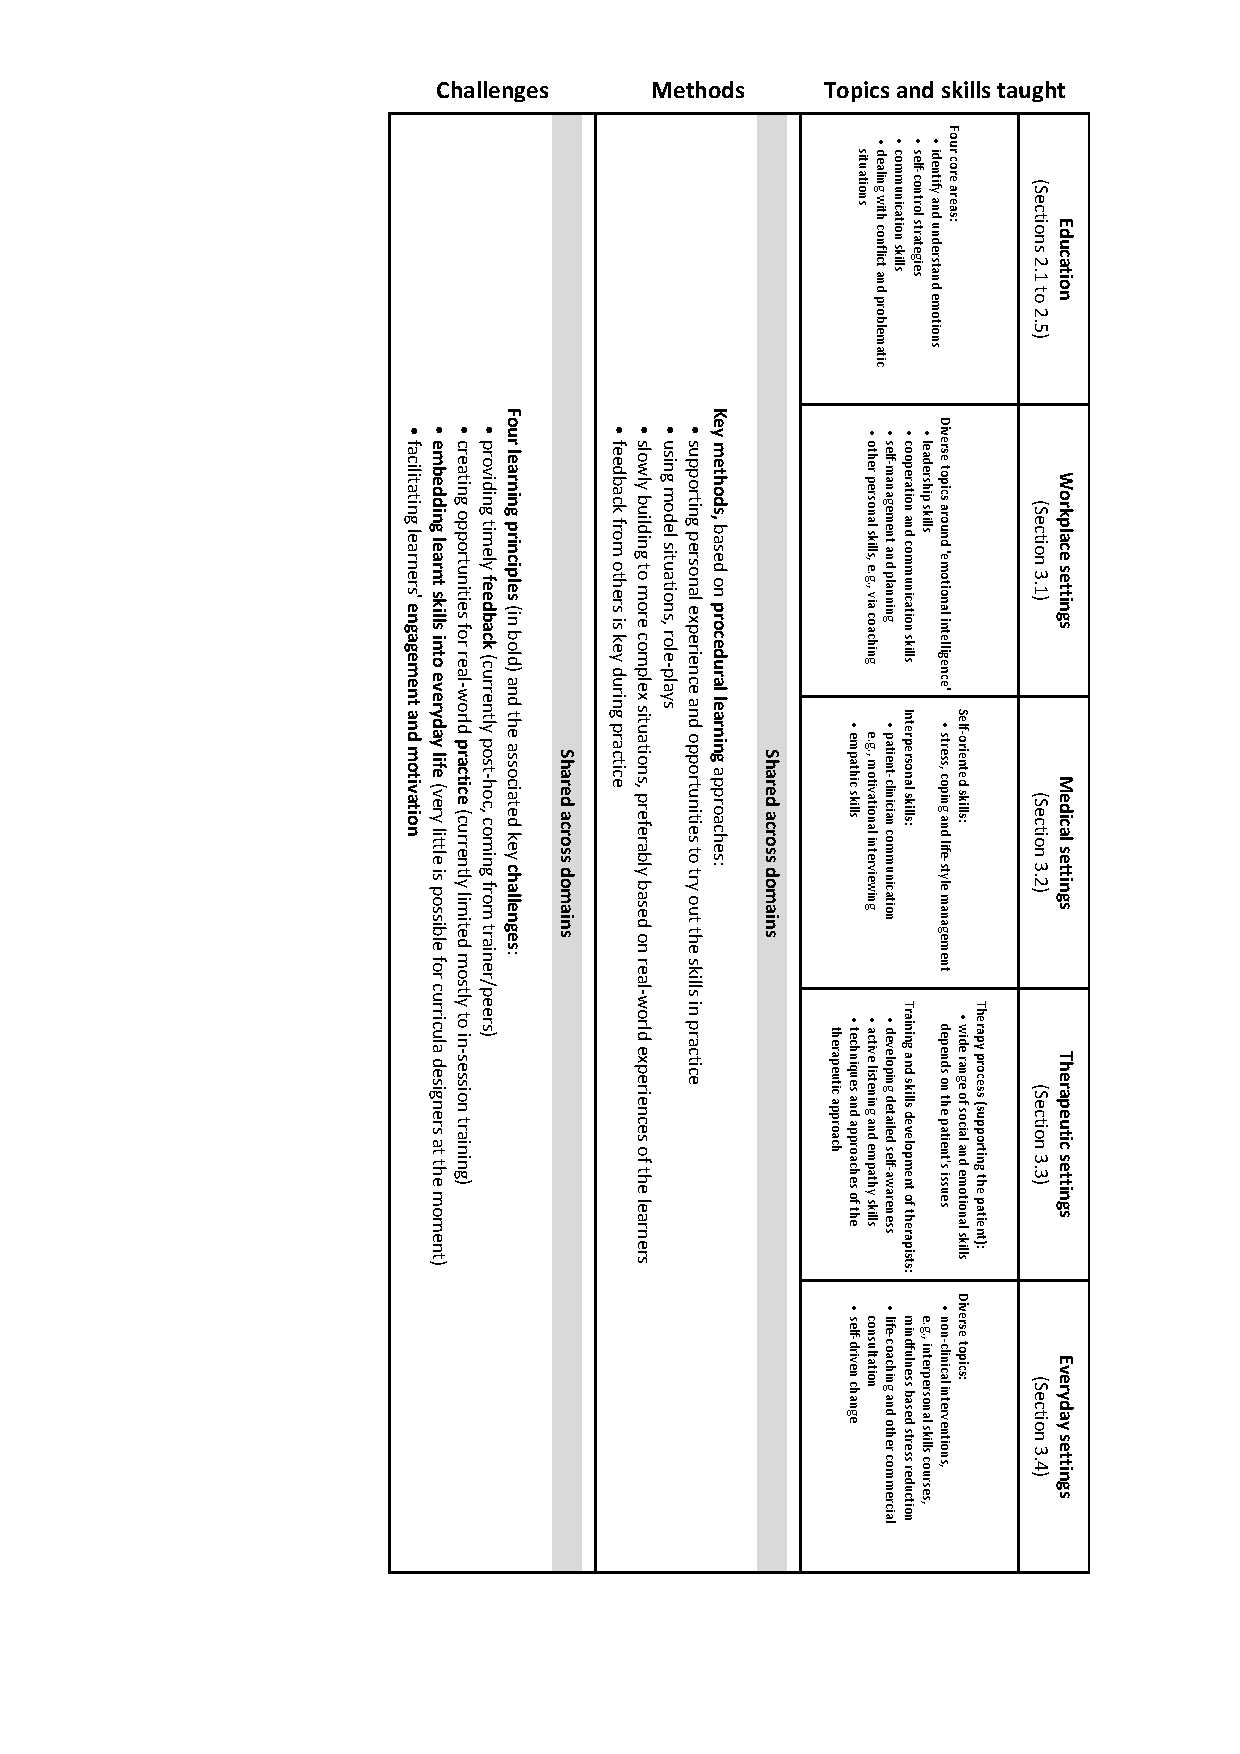
\includegraphics[height=\textheight]{images/SummaryResults}
	\caption{Overview of the key distinctions and similarities}
	\label{fig:SummaryResults}
\end{table}
\fi
%


% }}}
\fi

%{{{ SECTION -  Life skills courses in education 
\section{Life skills courses' contents within education}
\label{sec:SEL}
We start by reviewing the methods, topics and approaches used by SEL curricula in education to teach social and emotional skills. This provides grounding for the next three sections that link the existing SEL practices and challenges to HCI work.
				%  The goal here is to build an overview across the curricula of what gets taught and how, and then use this structure to outline the potential for HCI research. 
%        The overview in this section is deliberately kept quite descriptive and without explicit links to HCI research, although our review process aimed to identify and foreground aspects and challenges relevant to HCI perspective.
%
%We first outline the reasons why we chose SEL for schools as an exemplary domain (section~\ref{sec:reasons}), and describe the literature review methodology (section~\ref{sec:methodology}), before 
        %
%We then present the \emph{methods} used in teaching of social skills in education (section~\ref{sec:methods}),  as well as the key \emph{topics} that  get taught (section~\ref{sec:blocks}), including specific examples from various curricula. 


% {{{ SEL for school
\subsection{SEL in schools as an exemplary domain}
\label{sec:reasons}
%We chose social and emotional learning (SEL) in schools as an examplary domain we review in detail and return to other domains in the next section. %which serves as the basis for a \rephrase{system} of goals, methods and building blocks that encompasses also other domains.
%We outline the reasons for this choice below: 
Social and emotional learning in education is a mature field, with numerous well-researched and evidence-based approaches, and is particularly interesting for a number of reasons:

First, skills taught in school-based curricula are those that have been identified by psychologists and educators as crucial, not only to development in childhood and teenage years, but more importantly as key skills for adult life \cite{Greenberg2010}.  As such, school-based SEL encompasses the core set of skills needed for all domains of life and into adulthood. They also focus on a large span of ages, from kindergarten to high-school education.   %Further, many other life skills domains will often assume some basic level of these skills to have been developed during childhood, and focus then on the deepening of particular subsets of social skills specific to the social and emotional skill needs of the domain.  % as shown in sections below.

Second, SEL has an extensive 20+ years of history of peer-reviewed programs, which have already been deployed to millions of pupils. This suggests the potential for a considerable real-world impact for any HCI technology that would get included, or inform, SEL programs implementation. For example, \citeN{Durlak2011} reviews 213 program intervention studies encompassing more than 270000 students of all ages, with the interventions conducted over several years. Some studies have their effects tracked for even longer periods of time, as is the case for \citeN{Muennig2009} who recently presented a 37-year follow-up study on the results of a randomized controlled trial of High/Scope Perry Preschool Program conducted in 1962. Moreover, federal programs support further uptake of such curricula in the US \cite{CASEL2013}. 

Third, recent academic reviews have analysed the evidence-base for the effectiveness of SEL programs and find measurable and significant positive effects of SEL in randomised trials, e.g., \cite{Durlak2011,Greenberg2010,Weare2011}. In particular, the social and emotional skills curricula lead to improvements in  academic performance and the taught skills areas. For example, \citeN{Durlak2011} report an average of 11\% improvement in academic performance, and 25\% improvement in social and emotional skills; as well as positive impacts on many other aspects of behaviour such as mental health \cite{Adi2007a}, violence prevention \cite{Mytton2006,Adi2007b}, conflict resolution \cite{Garrard2007},  and reduction in bullying \cite{Vreeman2007}. %For more detail see e.g., \citeN{Weare2011} who provide a meta-review of 52 reviews in this domain, concluding that the interventions ``had wide-ranging beneficial effects on individual children and young people, on classrooms, families and communities and on an array of mental health, social, emotional and educational outcomes''.

%Despite these achievements, the SEL literature also highlights several problem areas which curricula struggle with---such as the embedding and transfer of learned skills out of SEL training classes and into everyday situations. As we will argue, this suggests, in combination with existing HCI work, that inclusion of digital technology could further enhance and improve the effects and efficiency of curricular training.

%Lastly, the topic also gains increasing political support in the US and Europe, suggesting that social and emotional learning programs for schools might be soon \rephrase{common}. As such, SEL itself provides a novel design space for HCI that could have a strong impact on everyday life and direct real-world applications. 

 %Example of this might be the emphasis on communication skills in medical domains or workplace.


% }}}

        
% {{{ Methodology
\subsection{Literature review methodology}      
\label{sec:methodology}
A large number of systematic reviews of SEL literature already exist, mainly with the focus on meta-analyses of measurable effects and long-term impacts of the curricula (e.g., \cite{Durlak2011,Weare2011,Adi2007a,Greenberg2010,Elbertson2009,Payton2008}). 
%
We build on these and approach the topic with a complementary HCI perspective in mind, aiming to identify the SEL challenges that could be addressed by technology. %To do that, we drew out processes, methods and topics commonly used within curricula, and  the challenges the SEL curricula currently face. 

As such, we analysed the contents of selected curricula, in addition to following references cited by the academic reviews above. This analysis was done by first creating summaries of individual curricula, collating these in mindmaps to draw out related topics, methods and approaches, and finally iteratively identifying the common aspects across curricula and domains. 
%
Given the large number of available curricula for the educational domain, we based our review on a set of curricula selected by the 'Collaboratory for Academic, Social and Emotional Learning' (CASEL)\footnote{\url{http://casel.org/}}, which is a non-profit organisation supporting research and application of social and emotional learning in education, co-founded by leading figures in the academic field. 

In particular, we drew on curricula identified in two CASEL 'guides': the \citeN{CASEL2003} guide reviews 80 SEL programs selected by a rigorous procedure, highlighting 22 of
% P: the first footnote speaks about the programs in general, the second about those that have been highlighted. But I agree it is confusing and should be combined together
 these as particularly well-designed. Each of the 80 programs is described, rated on 15 aspects and linked to academic literature evaluating its effects. The newer version of the guide, \citeN{CASEL2013}, focusses primarily on preschool and elementary school programs, recommending 23 programs.
%\footnote{Out of these, 14 have been already included in the 2003 version, and 9 are new: 4Rs, Competent Kids, Incredible years, MindUP, OpenCircle, Raising healthy children, RULER, Too Good For Violence, and Tools of the Mind.}. 
%
We first systematically analysed the descriptions of all programs in both guides, and continued with more detailed examination of the programs highlighted in either version of the guide (i.e., 34 programs altogether\footnote{Eleven programs selected in CASEL 2013 guide were already selected in the 2003 edition, leaving twelve newly described ones, leading to 34 programs altogether (22+12). \GeraldineTODO{LIST\ THESE\ BY\ NAME\ HERE\ AS\ COMPLETE\ LIST?}}), as well as the academic literature available for each of these programs as referenced in the guides, as long as it was accessible through the libraries of three major universities (yielding 66 academic articles altogether). We also included any course materials and descriptions of the programs that were available on the internet. Finally, we included a number of books on creating SEL curricula in the context of education \cite{Maree2007,Elias1997,Pasi2001,Zins2004,Patrikakou2005}. 





%%Section~\ref{sec:linkDomains}  showing how the identified competencies and methods play out also in the other domains. 
% }}}


% {{{ Teaching methods in SEL for schools

%\vfill ~ \pagebreak
\subsection{Methods for teaching SEL in education -- experiential learning}
\label{sec:methods}

Curricula share the understanding of social and emotional skills as highly complex abilities, drawing also on subconscious processing \cite{Ambady2010,Lieberman2000}. As such, social and emotional skills are based on \emph{procedural} rather than declarative knowledge \cite[p.288]{kruglanski2007social}. Moreover, the key ability of most social and emotional skills is to be able to react appropriately even within `hot' moments, i.e., situations  when the learner is overwhelmed with emotions, and/or the importance of the situation, or just has a very short time to react (e.g., heated conflict). During such moments, the ability of conscious, analytical thought is often diminished \cite{Wyman2010,leDoux1998}, emphasising the need for learning skills that operate on a procedural basis.

%In other words, even if students already have intuitive knowledge on how to react in a social situation, it is problematic to explicitly articulate the processing rules by which they came to these conclusions. Examples of similar dependency on procedural skills can readily be found  in other aspects of our life such as language use, where we know which form in our native language is correct but not necessarily why (``it sounds better''); or in social cognition where people are, for example,  very sensitive to correct proportions of human face, but are not able to explicitly articulate even the most basic ones correctly \cite{Lewicki1987}. 

  

%\subsubsection{Teaching methods used in SEL}
The core of most curricula is a set of SEL focussed, structured classroom lessons \cite{jones2012social}, usually 25-40 minutes long and administered once a week throughout the whole school year (or multiple years). During these lessons, curricula use predominantly active instructional techniques drawing on skill-based and experiential approaches. They employ a wide range of methods such as modeling, role-play, performance feedback, dialoguing, positive reinforcement, vignettes, play and games; as well as other approaches such as portfolios, expressive arts, exhibitions, or group projects -- see also Fig~\ref{fig:methods} for an extended list. Through these methods, curricula aim to include extensive examples and opportunities for personal experience and practice, combined with extensive feedback and opportunities for reflection on behaviour and progress. When teaching a complex interpersonal skill such as conflict resolution, curricula break the skill down into smaller molecular sub-skills and focus first on simple model situations. These can be explored by role play (e.g., specific situations such as asking permission to join a game), slowly building up to more complex, but scaffolded situations (e.g., in-class, teacher facilitated resolution of a peer conflict), and eventually to encouraging learners to apply the skills out of the classroom in everyday situations. Repeated practice and extensive feedback from the trainer and peers are critical components in every step of the process in the classroom. 

Once a skill is mastered within the lessons, the key emphasis is then on its \emph{transfer} out of the classroom into everyday contexts to promote maintenance and generalisation \cite{Elias1997,Maree2007,Pasi2001}. This is however one of the current \emph{critical challenges} SEL curricula face, and also one of the main areas where HCI could support SEL (cf. Section~\ref{sec:embedding}). Although curricula highlight the need to support opportunities for the learners to practise their new skills in real life situations outside of the classroom, they have very limited strategies to do so, especially as the scaffolding offered by the teacher in class is no longer available. The current methods curricula use to support transfer are mainly various activities to increase awareness and remind learners about their skills on the school grounds (e.g., posters around the school), and attempts to enlist the help of their social networks outside of the learning environment such as their parents and other school personnel (e.g., through organising workshops, or sending letters to parents with suggestions how they can reinforce the learning at home). Providing students with activities and exercises to attend to at home or other locations is also common. Overall, however, the curricula struggle to find ways in which to deliver direct support for students outside of the immediate SEL lessons \cite{jones2012social,Maree2007}.  


Curricula are clear that the methods used must be developmentally appropriate for the age of the children, and the skills learned. For example, incorporation of fantasy play or puppets as role models and curricula protagonists has been very successful for younger children (e.g., kindergarten to K-3), who can relate to them easily  \cite{Webster-Stratton2004}. In contrast, group discussions, journal writing and workshop activities are more commonly used with older children and teenagers \cite{dejong1994}. However, specific key methods such as role-playing, modeling, positive reinforcement, and direct and indirect instruction are used throughout in various guises. 
\todolater{Add example from SecondStep pointing to use of videorecordings and workshops for parents ==> highly useful... See \cite[p.88]{Elias1997}.}


%\todo{This is probably not good enough at the minute -- would need one p:aragraph about the parent/community involvement in more detail, if saying that this is an increasing focus or similar blah. Additionally, this combined the embedding into school life, and embedding into everyday, which is probably not what we want?}

\begin{figure}
  \centering
	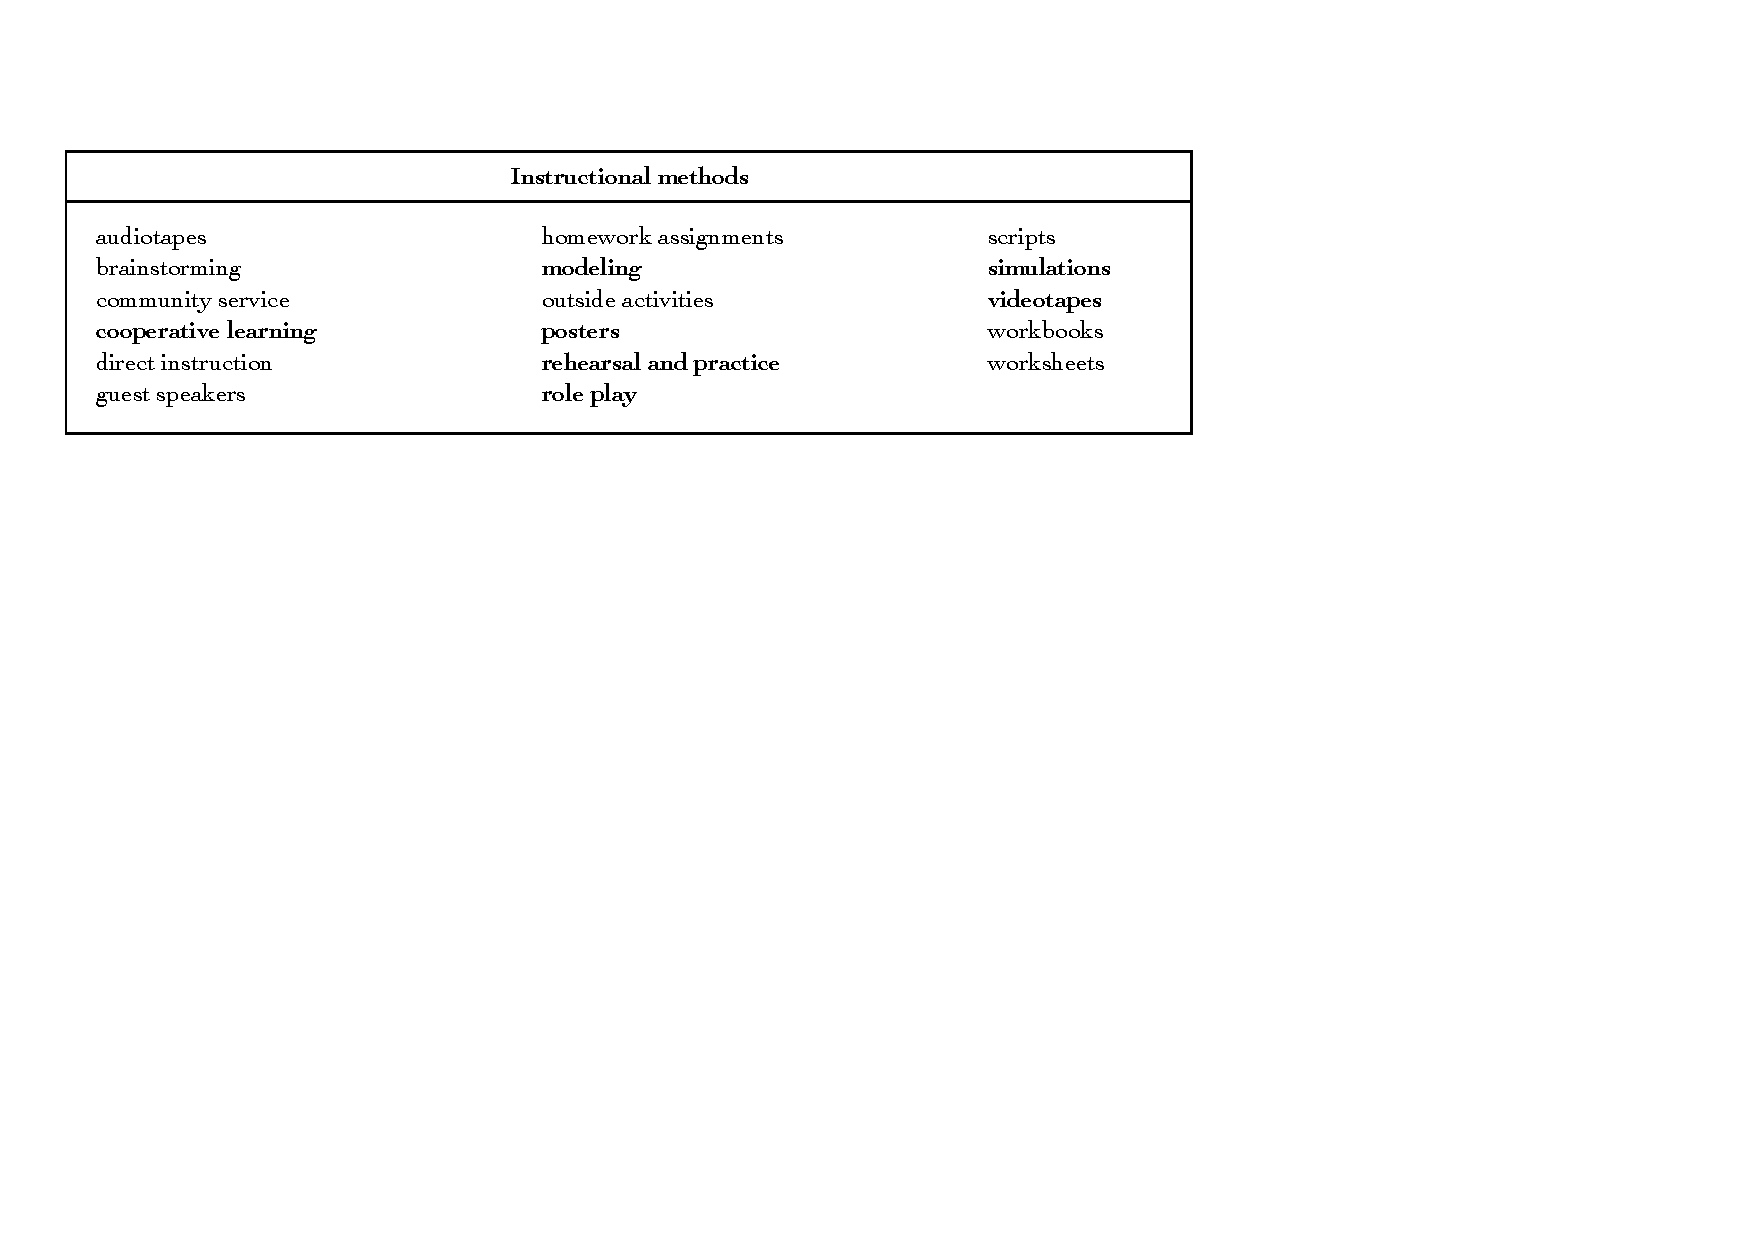
\includegraphics[width=.98\textwidth]{images/Elias-methodsList}
	\caption{Instructional methods used in SEL courses (modified from \cite[p.109]{Elias1997})}
	\label{fig:methods}
\end{figure}


%\qq{\cite{Webster-Stratton2004}}{Some strategies that will help young children learn and retain new information include: (1) provide many examples (in different media) of the same concept (videos, role plays, games, cue cards); (2) post cue card pictures in strategic areas to remind children of key concepts (eg, sharing cue card in big block area); (3) role play with puppets (common scenarios such as being teased, rejected, or making a mistake); (4) reenact videotaped scenes; (5) use Dina andWally's detective storybooks to discuss key ideas and generate prosocial solutions; (6) play games designed to practice key concepts (eg, playing “Wally Says”); (7) rehearse skills through activities; (8) give homework to practice skills (ie,Dina's Detective Homework Manual); and (9) send letters to parents asking them to reinforce the skills children learned that week.}

%\qq{\cite{Webster-Stratton2004}}{List of approaches: puppets as models, Live and videotape modeling methods, role-playing and practice games, Helping children learn and remember concepts, Practice activities- coeaching/cueing/reinforcing, integration of affect+coginition+behavioural components, Fantasy play, promoting skills maintenance and generalisation}


% {{{ Common theoretical models
\subsubsection{Common theoretical models}
There is no single theoretical model that would be universally agreed upon by the existing SEL curricula to ground the learning process \cite{Payton2000}. Instead, curricula build on several complementary theories that each have robust evidence of positive effects\footnote{This is similar to psychotherapy domain, where a number of schools co-exist in parallel, each building on different theoretical groundings.}. 
Some of the most prevalent theoretical approaches are: (i) systems theory, which views SEL learning as embedded in the broader community and aims to systematically create a comprehensive climate for teaching SEL not only in the class but also in the school and local communities more broadly; (ii) psychoanalytic theory, which works with how conscious as well as unconscious (unrecognised) emotions shape how we act or learn, and who we are; and (iii) cognitive behavioural theory as base for primary prevention and the core skill based techniques such as modeling or role-play \cite[p.65]{Maree2007}).

However, despite different theoretical groundings, there is still a considerable overlap among these models in the competencies to be learned (as described in the next section), and a shared set of guidelines on what makes curricula effective. In particular, curricula should take a wide scope both in terms of methods and skills learned, build on a clear theoretical framework, use a comprehensive approach that integrates affective, cognitive and behavioural dimensions, and promote generalisation of skills \cite[p.119]{Elias1997}. Additionally, the literature highlights that piecemeal programming efforts, such as one-off workshops, are much less likely to be effective \cite[p.13]{Zins2004} than comprehensive programs.


\todolater{Outline the theoretical background of PATHS, Incredible Years and RULER. What does this mean for technology?}




% }}}

%}}}


% {{{ Topics in SEL
\subsection{Goals of SEL learning}
\label{sec:blocks}



%Whereas the previous section focussed on methods and the general approaches taken to teach social and emotional skills (i.e., "how"), this section focuses on the content, i.e., "what" gets taught. %We aim to outline the commonalities among curricula in terms of the topics taught, the exercices/approaches to do so, and the order in which the topics are learned. % Similarly to above, we draw on thorough perusal of literature describing the twenty-three interventions selected as effective by \citeN{CASEL2013}; as well as other related literature.
%

A set of five core competencies is widely accepted within the educational community \cite{Zins2007,Durlak2011,CASEL2003,CASEL2013} as a good description of the general goals shared by most of the existing curricula, regardless of underlying theories. We quote these competencies and their brief descriptions as per \citeN{Durlak2011}:
%

\begin{figure}
  \centering
	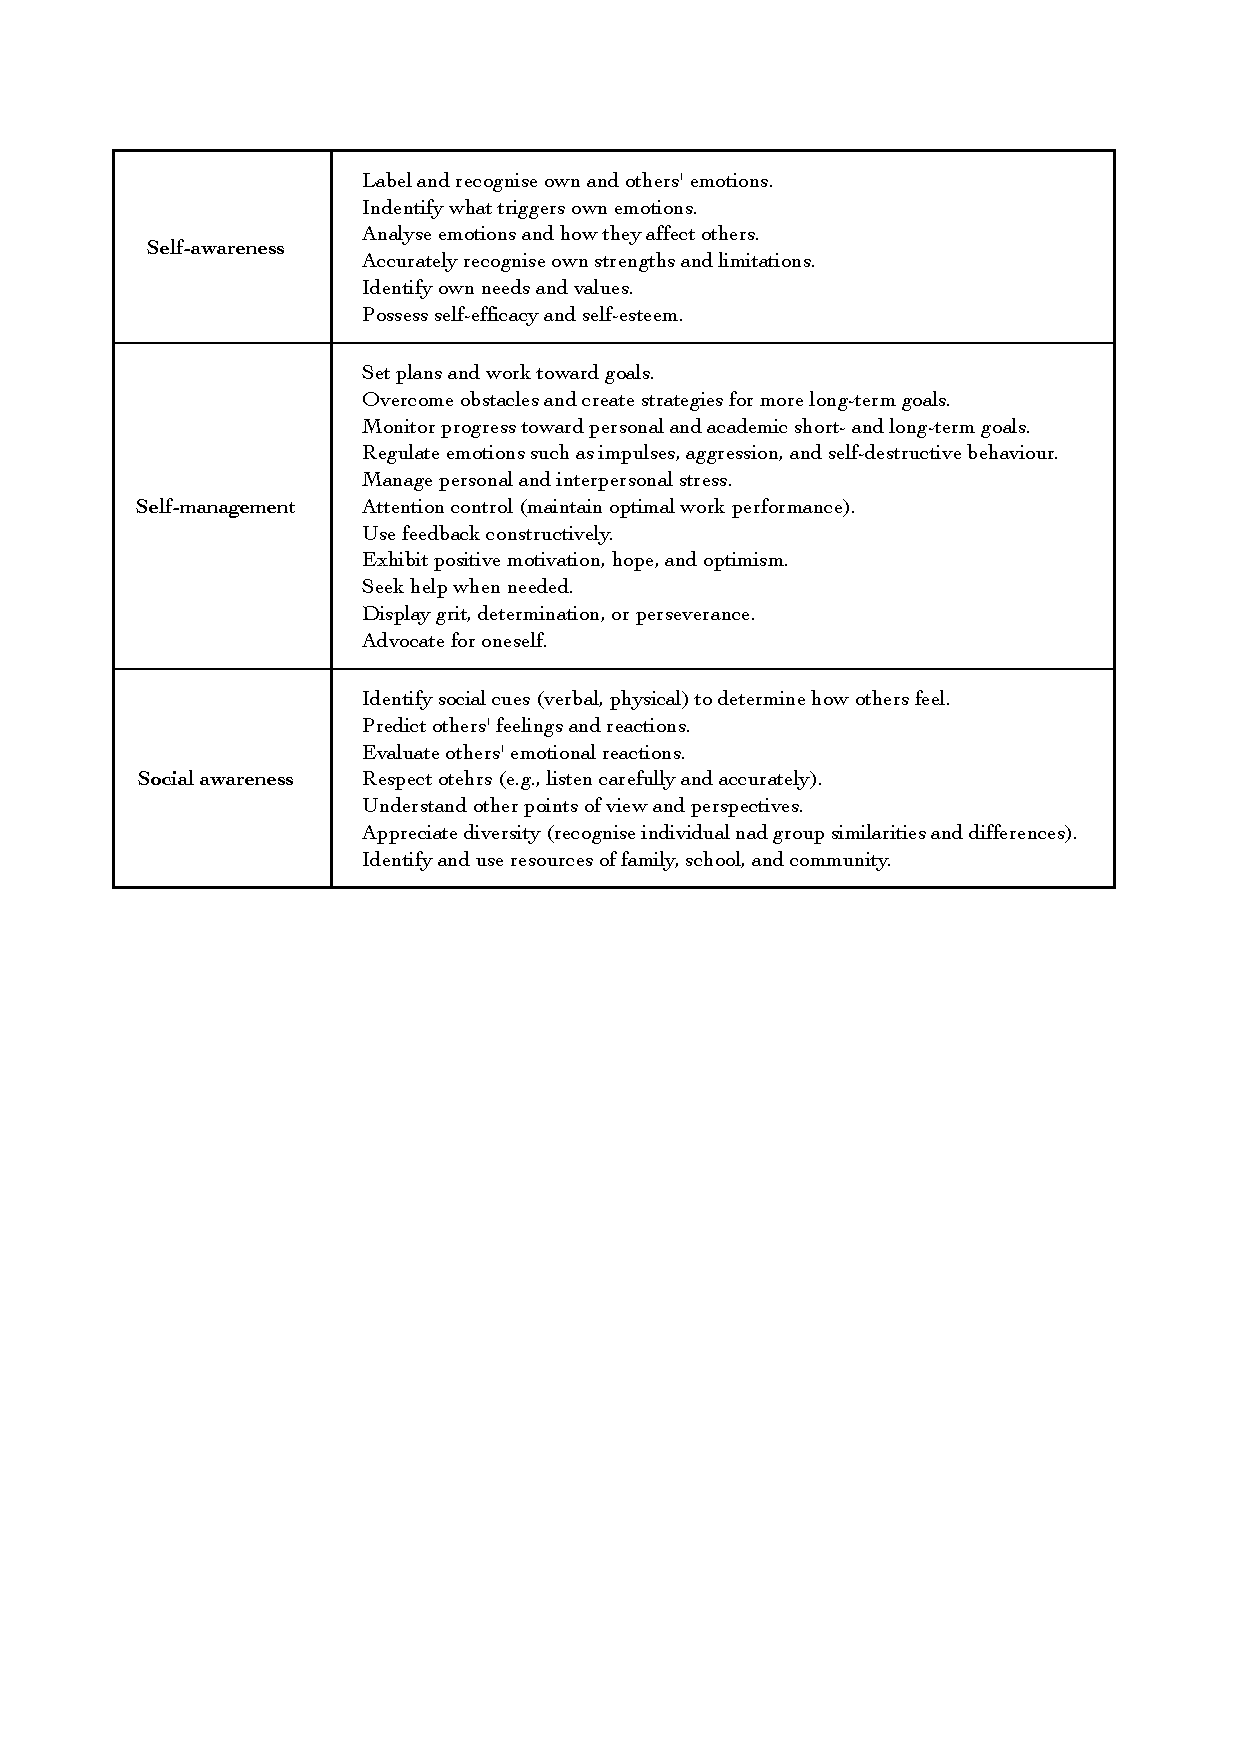
\includegraphics[width=0.48\textwidth]{images/Skills-list1}
	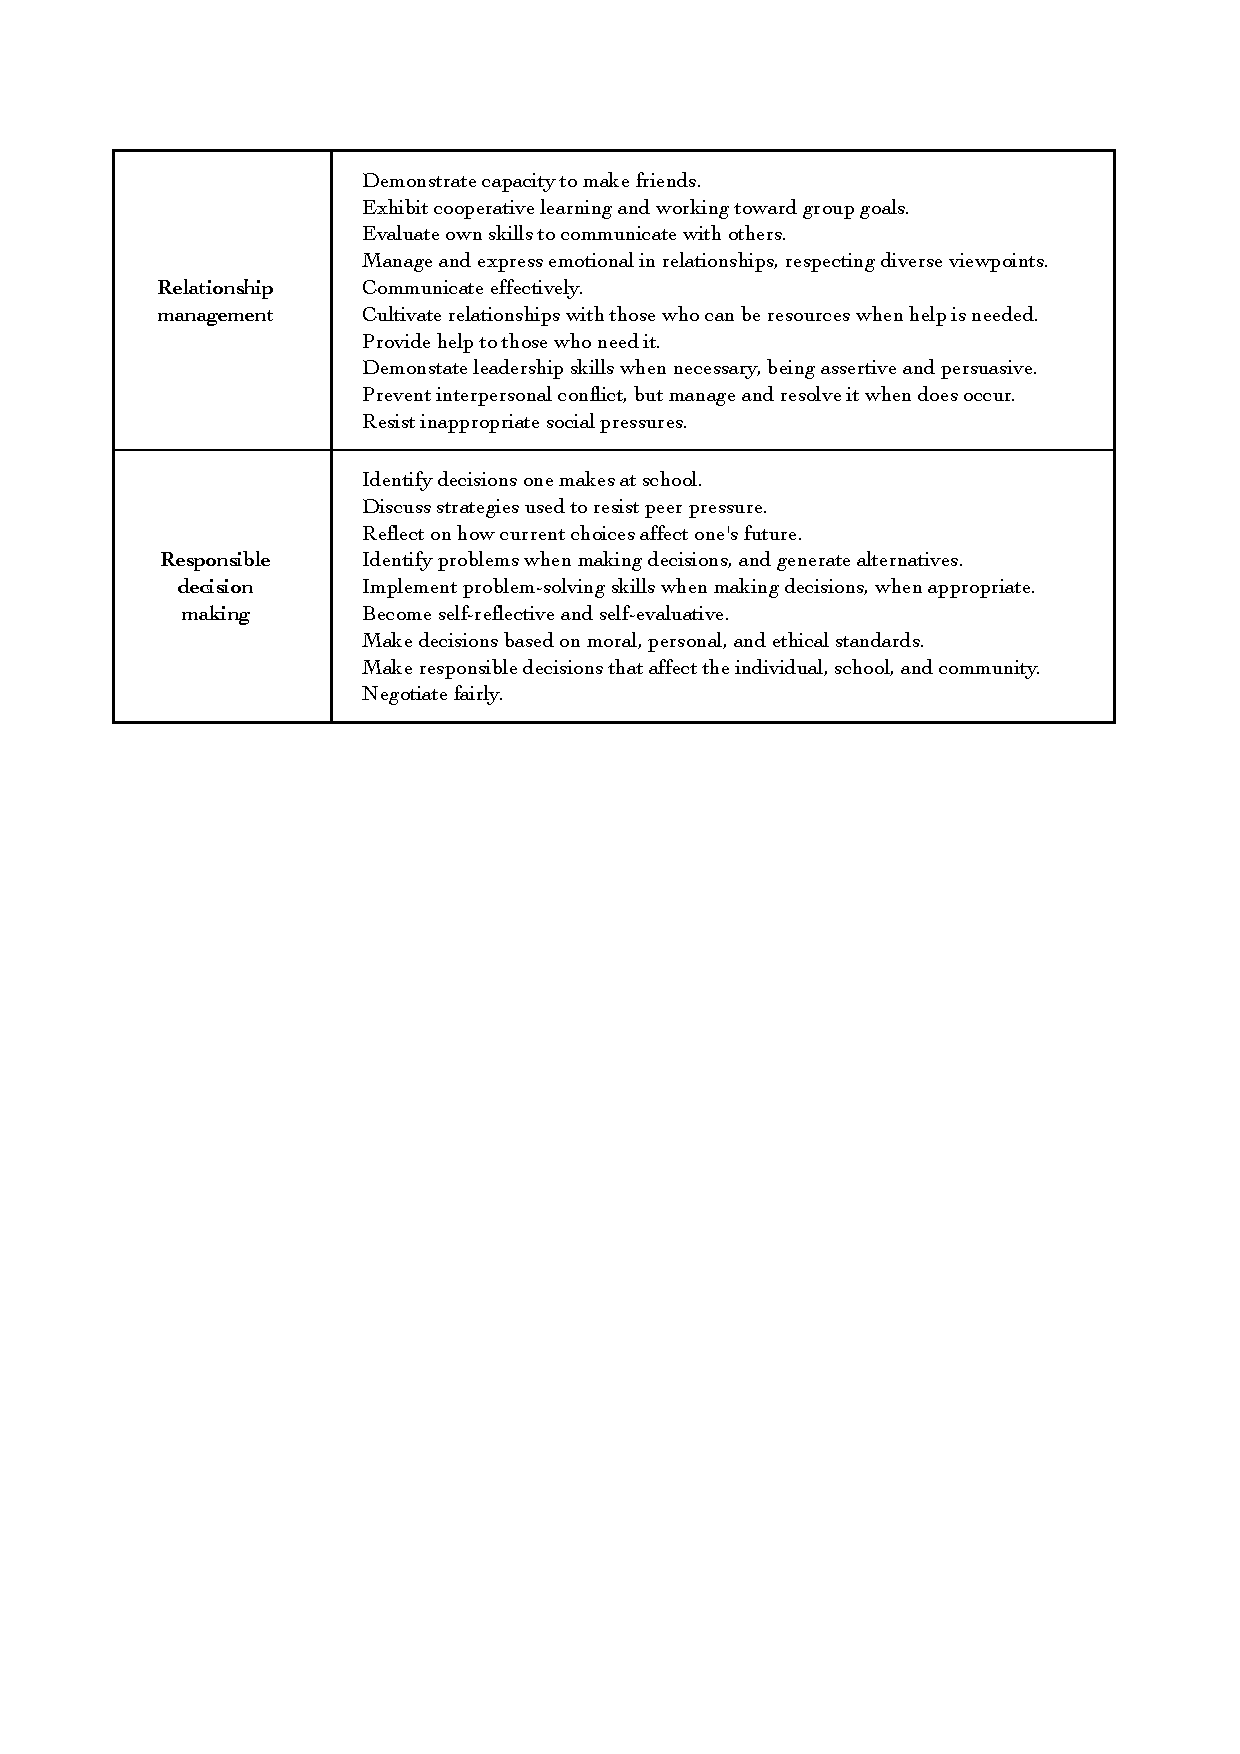
\includegraphics[width=0.48\textwidth]{images/Skills-list2}
	\caption{Exemplary list of skills relevant to individual competencies (from \url{http://www.gtlcenter.org/sel-school})\Geraldine{GF: NOT READABLE}}
	\label{fig:skillsList}
\end{figure}


%\todo{Not a good place for this? .. where does this go?}
%In other words, they provide a good description of the goal state (what SEL aims to achieve), and 
%
% serving as the key overreaching social and emotional skills that SEL curricula teach and promote. 
%


\GeraldineFIXNEW{ GF NOTE: possessive apostrophes below didn't print out in my pdf version}
\begin{itemize}
        \item {\bf Self awareness: }
                        The ability to accurately recognize one's emotions and thoughts and their influence on behavior. This includes accurately assessing one's strengths and limitations and possessing a well-grounded sense of confidence and optimism.
        \item {\bf Self-management: }
                         The ability to regulate one's emotions, thoughts, and behaviors effectively in different situations. This includes managing stress, controlling impulses, motivating oneself, and setting and working toward achieving personal and academic goals.
        \item {\bf Social awareness: }
                         The ability to take the perspective of and empathize with others from diverse backgrounds and cultures, to understand social and ethical norms for behavior, and to recognize family, school, and community resources and supports.
        \item {\bf Relationship skills: }
                        The ability to establish and maintain healthy and rewarding relationships with diverse individuals and groups. This includes communicating clearly, listening actively, cooperating, resisting inappropriate social pressure, negotiating conflict constructively, and seeking and offering help when needed.
        \item {\bf Responsible decision making: }
                        The ability to make constructive and respectful choices about personal behavior and social interactions based on consideration of ethical standards, safety concerns, social norms, the realistic evaluation of consequences of various actions, and the well-being of self and others.
\end{itemize}

However, these core competencies comprise complex, interrelated abilities and it is not possible to teach any of the competencies directly -- see Figure~\ref{fig:skillsList} for examples of the range of skills related to individual competencies. 
Instead, each curricula helps learners progressively develop these competencies, building up from smaller sets of 'molecular' skills. 
%}}}

% {{{ How are competencies taught?
\subsection{How are the competencies taught}
We identified four sets of such molecular skills that consistently appear in most of the curricula, and across all age ranges. Our goal is twofold: to provide an initial 'feel' for progression and topics taught in SEL; and to set up explicit examples that can be used in later sections to tie some of the existing HCI research to the approaches presented here.


\begin{enumerate}
        \item identifying and understanding emotions (own and of others);
        \item managing own emotions;
        \item developing communication and relationship skills;
        \item dealing with conflicts and problematic situations.
\end{enumerate}
 % Once mastered, these skills feed into the core competencies described in previous section, as shown at Figure~\ref{fig:strmap}.       
%Although the exact approach, terminology or exercises used by a particular curriculum can differ from others, there is substantial similarity in the focus and emphasis on these sets of skills across the literature.
 
Each set thus subsumes a number of simple situations or skills (e.g., being able to identify becoming angry) and ways to train these (e.g., training learners to notice physical changes in their bodies, such as associated with feeling angry).
Moreover, these topics build on each other in a sequential manner: The ability to identify and understand emotions is a key pre-requisite for managing own emotions (without knowing one's own emotions, one cannot control them), which is in turn needed for keeping relationships (appreciating the perspective of another, not jumping to conclusions) etc. As such, they are taught in the order as shown in Figure~\ref{fig:depfoc}. 
%
We describe each topic in more detail in a respective subsection below, illustrating the descriptions with examples of specific activities from selected curricula.  Figure~\ref{fig:strmap} then maps how the four topics contribute to the core competencies. 




 
\begin{figure}
  \centering
        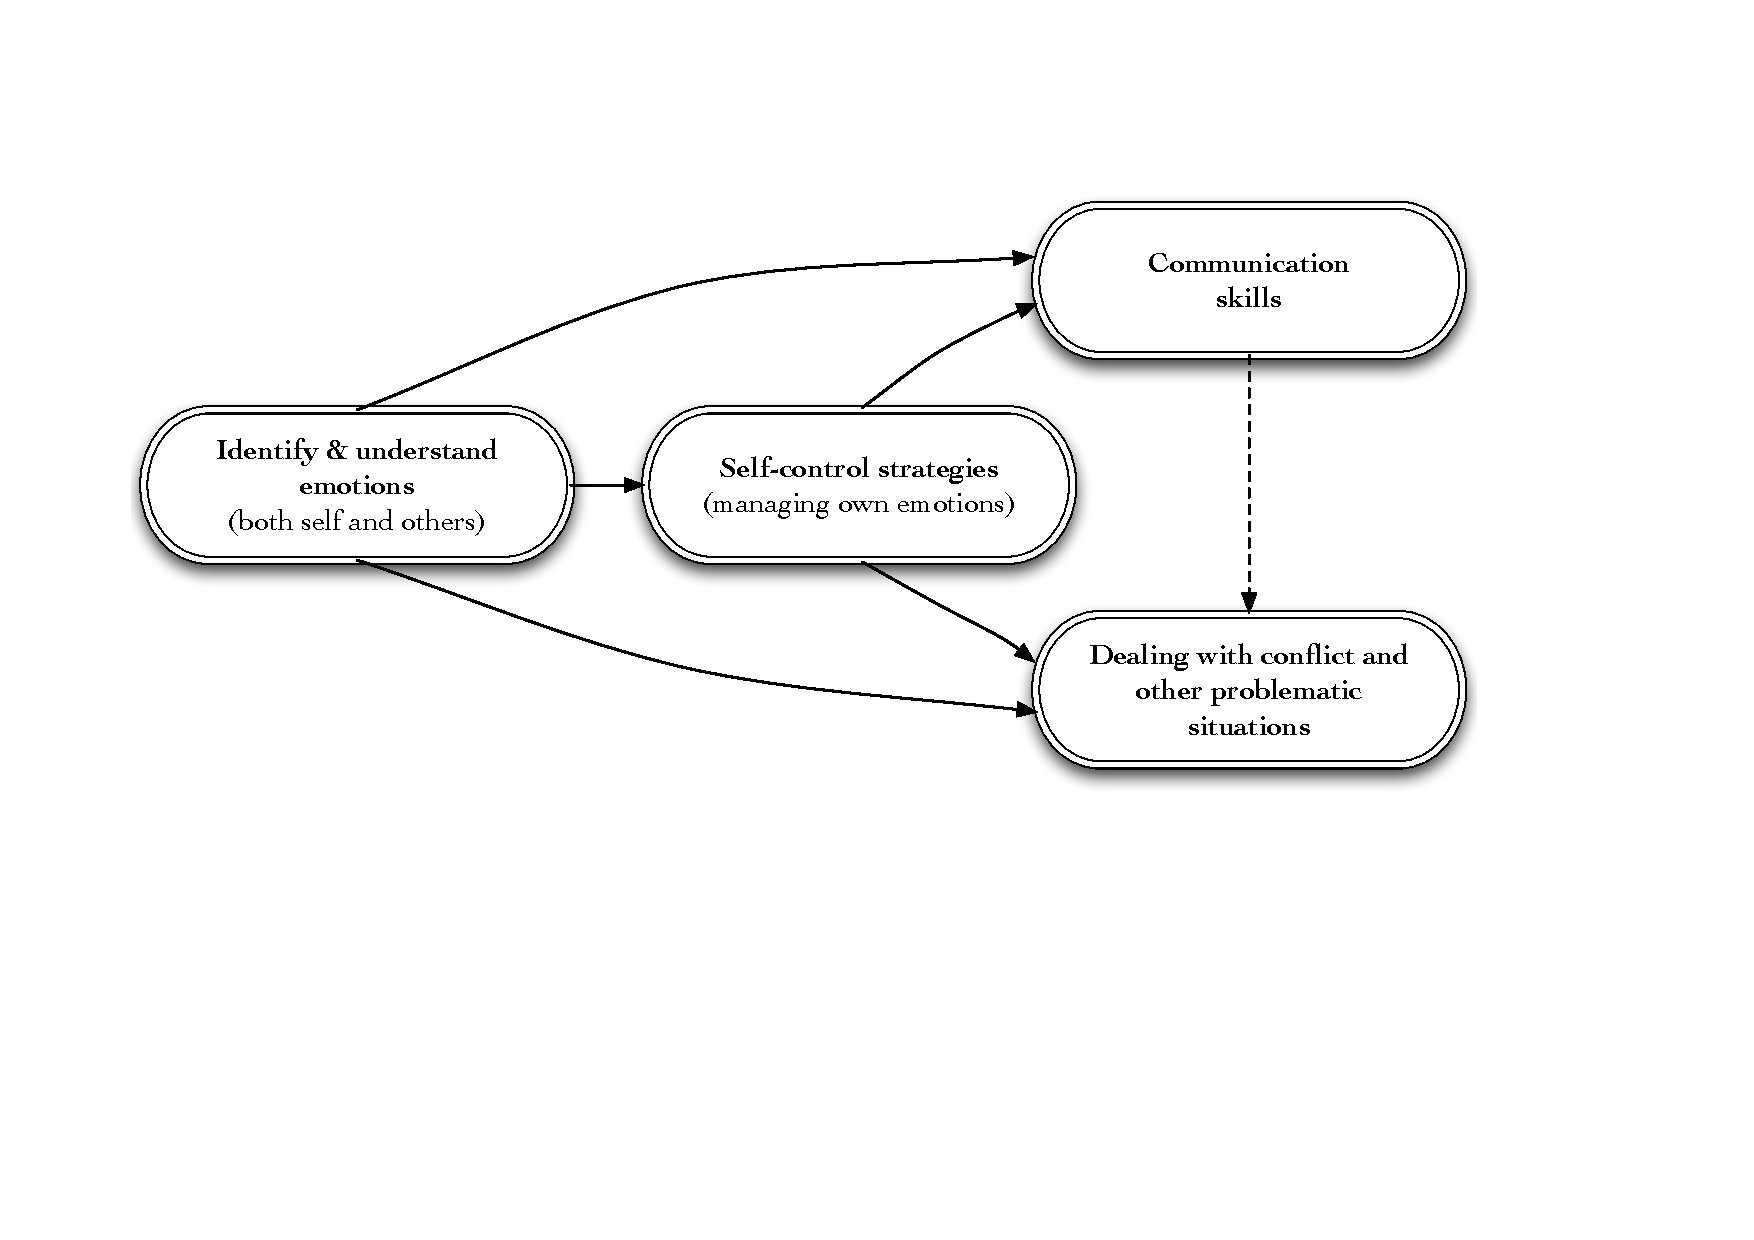
\includegraphics[width=\columnwidth]{images/BuildingBlocks.pdf}
        \caption{Summary of the identified key topics in SEL in education and their dependencies.\GeraldineFIX{G: make clearer that this represents your summary of key topics and dependencied}}
        \label{fig:depfoc}
\end{figure}

\begin{figure}
  \centering
        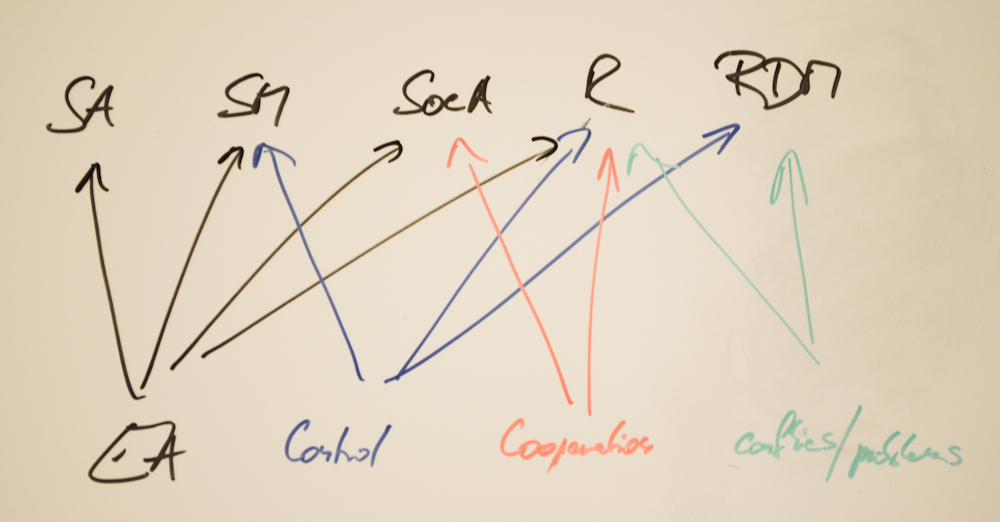
\includegraphics[width=0.9\columnwidth]{images/strategiesMapping}
        \caption{Mapping of topics to core competencies}
        \label{fig:strmap}
\end{figure}


%\renewcommand{\labelitemi}{$\cdot$}
\subsubsection{Identifying and understanding emotions} 
        %\setlength{\itemsep}{0cm}%

  %\setlength{\parskip}{0cm}%
The ability to identify and understand own and others' emotions is a prerequisite of most other social and emotional skills. A key goal is developing the emotional awareness of learners, which is the ability to differentiate, name and notice subtle changes of emotions. Curricula\footnote{Curricula including content on identifying and understanding emotions are: Caring School Community, I can problem solve, Life Skills Training, PATHS, Peace Works, Quest (Violence Prevention Series), Open Circle, RIPP, Responsive Classroom, Second Step, SOAR, Social Decision Making and Problem Solving Program, 4Rs, Competent Kids, The Incredible Years Series, Michigan Model for Health, MindUP, RULER, Social decision making, Steps to respect, Too Good For Violence. {\bf 21 in total}} aim to train a practice of internal reflection, leading to continuous exploration of how they and others feel. Emphasis is also placed on making the distinction between acknowledging a feeling, and acting upon that feeling/urge. 
\GeraldineFIX{G: all the other subsections list the relevant curricula at the beginning of the section so maybe move the footnote with the list from end of section to here}

In particular, some of the curricula build on language usage, and especially on how use of language affects our thinking processes. Various exercises focus on developing the ability to identify emotions in both oneself and others, helping learners to become more reflexive and self-aware. As an example, the PATHS curriculum  includes physical ``Feeling Faces'' cards, which the child learners use to signal their current emotional state throughout the day \cite{Kam2004,Domitrovich2007}. Similarly,  the RULER curriculum uses popular stories to exemplify particular emotions, and to draw out distinctions among subtle variants of a specific one \cite{Reyes2012}. 
%
Another approach aims to support self-reflection by exploring and understanding how our bodies are affected by experiencing particular emotions. For example, children are helped to recognize their own feelings by checking their bodies and faces for `tight' or relaxed muscles, frowns, smiles, and sensations in other parts of their bodies such as butterflies in their stomachs. Matching the facial expressions and body postures shown on cue cards helps the children to recognize the cues from their own bodies and associate a word with these feelings \cite{Webster-Stratton2004}. 
%               
Emotions of others are explored through the ways in which they affect the tone of voice, body language etc. This is often incorporated as a game, e.g., developing the 'detective skills' to find out how others feel. Repeated   use of similar activities aims to help learners think more often about how they, and others, might feel in various situations. 
\GeraldineFIX{G: do you really mean constant ie no break???}



\subsubsection{Self-control strategies}
        %\setlength{\itemsep}{0cm}%
  %\setlength{\parskip}{0cm}%
Self control and management of own emotions is a key aspect present in many curricula\footnote{Life Skills Training, Lion's Quest, PATHS, Peace Works, Productive Conflict Resolution Program , Quest (Violence Prevention Series), Open Circle, RCCP, RIPP, Responsive Classroom, Second Step, SOAR, Social Decision Making and Problem Solving Program, Teenage Health teaching Modules, 4Rs, Al's Pals, Competent Kids, The Incredible Years Series, MindUP, Positive Action, RULER, Steps to respect, Too Good For Violence. {\bf 24 in total}} and the techniques used to develop self control build on emotional awareness.%, aiming to teach strategies for managing strong emotions once they are recognised. 

Various strategies and exercises aim to help participants to relax and/or calm down once a strong feeling is recognised. These are often based on various physical exercises such as muscle stretching and deep breathing techniques. Other strategies draw on verbal labelling, building on psychology and neuroscience findings showing that the act of consciously labelling an emotion by name (rather than ``just'' being aware of it) facilitates higher cognitive control over the emotional state \cite{Greenberg2006,Reyes2012}. Exercises training explicit acknowledgement of emotions, as well as thinking about what could be their cause, are often used. 
Specific strategies for anger management are particularly common, often combining both verbal labelling and physical relaxation exercises. An example is the ``Turtle technique'' \cite{Robin1976}, which is still used in a number of curricula (e.g., PATHS). In this technique, children are taught to ``withdraw into their shell'' (by pulling their arms and legs close their body and closing their eyes) at specified occasions such as when they feel increasingly angry. This is followed by a relaxation phase, where specific muscle groups are tensed and released. Once this technique is mastered, children discuss appropriate alternative strategies for dealing with stressful situations, now that they are able to consciously reflect and react to them. 
\todolater{For older children, self-control exercises focus on supporting personal management more broadly, such as promoting goal setting, self-motivation and grit.}
%\todo{Add a sentense around older students -- self-control as important to support motivation and grit}

\subsubsection{Communication skills}%Facilitating positive relationships},
Another set of activities focuses on building good communication skills and supporting positive interactions with others\footnote{While implicit in many others, this aspect is explicitly highlighted within the following curricula: Michigan Model for Comprehensive School Health Education, Peace  Works, Open Circle, RCCP, Responsive Classroom, Second Step, SOAR, Tribes, Al's Pals, The Incredible Years Series, MindUP, Positive Action, Steps to respect curricula. {\bf 13 in total.}}. The skills taught here aim at supporting respectful empathic communication and thus implicitly facilitating friendship relationships, and an ability to collaborate and avoid conflicts that could otherwise occur through misunderstanding. 

The emphasis is on teaching active listening, which is then used to facilitate teaching empathy. Other teaching strategies also focus on training of specific communication skills (e.g., giving and accepting compliments).
Exercises can include games to: induce collaborative activities; practise active listening, e.g., through listening to someone telling a story and then trying to rephrase it with as many details as possible; and disagree respectfully. These can include ways to subtly reframe a message into a form which is not threatening, such as in \citeN{ABER1998} where students are taught to acknowledge the potential mismatch between their and the other's perception of the situation (e.g., preferably saying "It seems to me you are not listening now.", rather than ``Why aren't you listening to me!'').%\todo{Stronger connection to building relationships needed?}

\subsubsection{Dealing with conflicts and problematic situations} 
Problem solving strategies and conflict management are the final topics of most curricula\footnote{Michigan Model for Comprehensive School health Education, PATHS, Peace Works, Productive Conflict Resolution Program, Quest (Violence Prevention Series), Open Circle, RCCP, RIPP, Responsive Classroom, Second Step, SOAR, Social Decision Making and Problem Solving Program, Tribes, 4Rs, Al's Pals, I Can Problem Solve, Competent Kids, The Incredible Years Series, Positive Action, Social decision making, Steps to respect, Too Good For Violence. {\bf 22 in total}}.  Violence prevention is commonly an important additional goal, as many of these curricula are designed  for all schools, including those with a high prevalence of aggression and weapon use. 


Students are often taught a particular structure of reacting to a problematic situation or a conflict.
%
A key approach is to help students process the situation on a cognitive level, despite the fact that conflicts tend to ignite strong emotions. For example, the PATHS curriculum includes a ``semaphore'', where the sequence of red-yellow-green indicates a "stop-think-proceed" process \cite{Kam2004,Domitrovich2007}. Such structured sequences always include and emphasise a goal setting and evaluation phase. Moreover, curricula aim to teach children and teenagers to recognise which conflicts might have arisen from misunderstanding, with perspective taking exercises forming the core approach. An example is exploring win-win negotiation (e.g., in RCCP) in a workshop format and providing suggested sequences for steps to take during disagreements (e.g., in Incredible Years).



% }}}

% {{{ Differences across grades
\subsubsection{Differences across grades}
\label{sec:ageDiff}
Curricula exercises are designed for specific grades/age levels, keeping in mind the developmental changes in abilities of the learners. For example, curricula for K1 students can aim to help the learners label and identify basic emotional such as fear or happiness, K4 students might focus on more complex emotions such as jealousy or embarrassment, and high-school students would be taught to draw on their more nuanced self-awareness to motivate goal-setting and critically assess their behaviour. Curricula also particularly highlight the increasing integration of cognitive, emotional and behavioural aspects that can be expected of students as they grow older. See, e.g., \citeN[p.133-138]{Elias1997} for more detailed information on the progression and detailed changes in skills foci. 

% }}}





%}}}
%}}}

% {{{ SECTION -  Supporting SEL with technology
\section{SEL challenges and opportunities for technology support}
\label{sec:HCIsupport}

Despite the success of curricula in promoting learning of social and emotional skills to some extent (cf. Section~\ref{sec:reasons}), the review of SEL literature also highlights areas where novel approaches are needed, or further improvements are possible. In the rest of this section, we outline three such exemplary topics---embedding of skills into everyday settings, promoting reflection, and providing mixed spaces for practice. Our choice of highlighting these particular areas was motivated by the extent of related HCI work that exists for each of these. This allows us to exemplify the potential for collaboration of HCI and SEL, and specifically point to existing HCI work that suggests how incorporating digital technology may help address crucial needs in, as well as open new opportunities for, SEL in education. 


%The review of SEL have clearly outlined the fundamental role of experiential learning in development of social and emotional skills.

%We now highlight embedding as the key aspect through which digital technology may address a crucial need within SEL learning. Moreover, we also highlight promoting reflective abilities and mixed learning spaces to support further practice as two other areas where, based on existing work in HCI, we argue use of digital technology could bring novel opportunities to support and enhance current learning.

\GeraldineFIXNEW{GF NOTE: do you need to make it clearer what the challenges are and then also be clearer that you are structuring this discussion more by relevant work in HCI than the SEL categories you pulled out earlier? Otherwise raises questions about why these categories for this discussion???}


%Note: 
%We choose a specific format for this session, we always outline a particular challenge/issue existing in the SEL learning, using these to provide exemplary ideas for possible technology support. These are however not intended to provide the solutions (as any solution would need to be tailored to the SEL program, age of children etc.), only to illustrate the possible areas where technology could be useful, and which could be designed for. 
%
%Especially for the embedding part, many of the proposed use-cases revolve around novel sensor and other tracking aspects (SSP). While the current state-of-art might not be robust and reliable enough to be directly deployable in SEL settings yet, we argue that existing studies suggest opportunities for these to be so in future; in addition such use-cases can serve as benchmarks for viability of the setting and thus provide important guidance for future development.




% {{{ Embedding
\subsection{Embedding of learnt skills into other settings}
\label{sec:embedding}
We start with what the SEL literature highlights as one of the key issues with existing SEL curricula -- i.e., the lack of support for transfer and 'embedding' of the skills students learn in SEL classes into their other real-world interactions, be that still within school (other classes, playground) or everyday behaviour within family and peer groups \cite{Maree2007,jones2012social,Patrikakou2005,Elias1997}. 
%
While such transfer of learned skills is the ultimate goal of all curricula, the current approaches are limited in scope and effectiveness. This leaves teachers (and curricula designers) struggling to directly influence the embedding of skills outside of the SEL learning sessions, be that in other classes, or outside of school completely.
%
For example, \citeN{jones2012social} summarise the situation as follows: \qqq{Perhaps most important, and often overlooked, is the fact that SEL programs are rarely integrated into classrooms and schools in ways that are meaningful, sustained, and embedded in the day-to-day interactions of students, educators, and school staff [\dots] Most SEL programs focus solely or primarily on what goes on in the classroom, but SEL skills are also needed on playgrounds, in lunchrooms, in hallways and bathrooms -- in short, everywhere. These non-classroom contexts provide vital opportunities for students to practice their SEL skills.}
%
\citeN[p.70-71]{Maree2007} further highlight the critical role of adults, both in and out of school, in the success of SEL training for students: \qqq{Many SEL efforts fail because long-term, coordinated plans and school-home partnerships are not developed. [\dots] [T]he efforts of school-based practice falter because educators are not committed to being ongoing, vital SEL role models. SEL involves not just the students in schools but also the adults in their lives: teachers, parents and the wider community. If these adults lack social and emotional competency, children will quickly notice the discrepancy between behaviors that the adults advocate for children and the actions that the adults take themselves.}


%As such transfer of learned skills from SEL-specific class exercises to other activities in and out of school is a clear key challenge for the existing curricula [ref,ref].

We argue that digital technology could support these efforts in at least two ways: First, by extending the learning support and scaffolding for learners beyond the SEL lessons, e.g., utilising mobile and sensor based technology. Second, through facilitating a wider community of support for learning of social skills, including the involvement of parents and teachers -- not only by connecting them to the learning content in the classroom, but also enabling vicarious learning so that they develop their own social and emotional skills. We outline each in more detail below.

% {{{ Supporting learners directly
\subsubsection{Supporting the learners  -- Transitioning the skills out of the SEL lessons}
\label{sec:Embedding-learners} ~ \\
When SEL skills are to be transferred beyond the SEL classroom lessons, the learners can no longer take the advantage of the direct scaffolding normally provided by the teacher and the lesson structure. This brings several difficulties for the learners to reinforce and apply their skills outside of direct SEL training. We particularly highlight the difficulties with (i) identifying moments when the newly learnt social and emotional skills could applicable, (ii) the lack of scaffolding and support to do so, and (iii) the need for 'space' to reflect and learn from the experience afterwards. 

%We start by discussing the specific setting around SEL in/out of classroom, and the  \todo{Can we fit the in class/out of class dimension into here directly? Or at least make obvious that we talk about specific, fixed location and a set of SEL learning that can be supported, and the ability to 'ask' students to volunteer and use particular gatgets (as opposed to random people with a mobile phone at a random location) -- should we have a little section on setting affordances upfront? }
%\todo{Highlight this aims to support a novel informational overlay over existing real-world interactions that provides scaffolding for re-inforcement and transfer or learned skills in other contexts. As such, will bring serious challenges for HCI research in terms of robustness etc.; however school and still learning settings might ameliorate some when compared to completely in the wild studies as described above. }

\paragraph{Identification of teachable moments}
When interacting during breaks, other classes, or outside of school completely, the learners encounter many occasions that are relevant to their SEL skills learning. However, the learners may not recognise such opportunities and instead revert to previous, negative behaviours (e.g., an angry outburst rather than a self-controlled reaction), especially if emotions are strong and no external guidance is available \cite[p. 56]{Elias1997}.  In such situations, it is thus not only difficult for the learner to apply the skills they have learned, but even to perceive these as such 'teachable moments'. This is one of the key differences to the SEL class setting, where it is the role of the teacher to facilitate and point out situations in which students could use their (new) SEL skills, and reinforcing them if they do. 
%
Curricula designers therefore suggest that all school personnel should \inqq{play an important role in actively encouraging and reinforcing the use of skills and attitudes they see displayed} (e.g., \cite[p. 56]{Elias1997}). This however requires the (possibly untrained) teachers to constantly strengthen and actively encourage use of SEL skills in addition to all their other duties. More critically, there is little opportunity for supporting the learners when the teaching staff are not around (and thus also making the students fully dependent on external guidance e.g., from parents). 

This points to the benefits of (and the need for) technology that could support the learners themselves in noticing and reacting to the relevant situations. For example, learning self-control is one of the key aspects of SEL; it relies strongly on identifying a problematic situation and then to calm down before it is 'too late' and emotions are already running high. One opportunity for technology in this setting can draw on the maturing HCI research on in-the-wild stress detection drawing on physiological data or speech prosody, e.g., \cite{Hernandez2011,Poh2010,Pina2014,Zeng2009,Ertin2011}. We envision that such data could be used to support the learners in becoming aware of their heightened arousal (e.g., through a private tactile reminder such as FitBit wrist vibration), which can serve as a cue to start the self-calming/self-control mechanisms taught in class. Earlier research in HCI suggests that providing such on-going subtle cues for facilitating awareness, and triggers that remind users to attend to intended activities can be useful to help users modify their existing behaviours \cite{Consolvo2009,Obermair2008}. Moreover, SEL designers have deep understanding of how best to work with such cues and triggers, once these are identified. An example of initial work in this direction is \citeN{Pina2014}, who designed a system for parents of ADHD children, delivering in-the-moment cues and strategies to manage stress during everyday activities.  Overall, the initial studies point to the potential of such technologies, but also point to many practical issues to be addressed, including whether such systems are robust and precise enough for immediate inclusion into the SEL curricula, and how could these be best embedded in the existing programs to most appropriately exploit this potential. 

\todolater{???Other similar opportunities for technology could be in supporting other learned topics such as prompting awareness of own emotions, }


%Similarly, this brings opportunities for novel tracking made available by recent advances in Social Signal Processing (such as detection of shouting or anger from speech intonation and intensity \cite{Vinciarelli2012}), should it prove robust enough for 

%\rephrase{Alternatively, technologies helping students identify learning moments could leaving detection on the learner but supporting better focus -- e.g,  through journalling and other reminder methods, digital technology has been shown to support the users paying more attention to activities of interest -- think of something like the noticing button, or young kids asked to take pictures of students engaging in 'supported' behaviours (e.g., lending toys, playing together ...)}




\paragraph{Scaffolding and structure to support training of skills}
Learning of skills is scaffolded in many ways within SEL training sessions:  (i) the scaffolding inherent in the activity itself, such as a prepared scenario for a role play that highlights a particular aspect to focus on; (ii) the teachers' presence and input into the activity, such as prompts guiding the development of the role-play, and feedback to students on their behaviour; and (iii) also the fact that this is a SEL training session, which brings a particular set of foci for the students including the explicit attention paid to SEL skills development. However, much of this scaffolding disappears outside of the SEL learning, even if the situation is still within a class setting (e.g., during a lesson in a different subject). 

% , but similarly in other curricula. Schools currently deploy posters around the school with the aim to support students' ability to remember and use these in the important teachable moments. However, these do not seem to be very efficient \ref{Cohen2006}.

This points to the opportunities for technology to provide just-in-time prompts, reminders and structuring, e.g.,  through mobile devices, to support the scaffolding of activities and help learners focus attention on SEL skills in play. 
%
Examples of such direct scaffolding methods that can be useful out of SEL classes include problem solving strategies such as the 'stop-think-proceed' semaphore in the PATHS program and the sequence of steps to resolve disagreements in the RCCP program, where each person is invited to share their perspective on the situation in turn. Within HCI, several projects have explored technology support for similar structuring as part of autism therapies. For example, the MOSOCO project \cite{Escobedo2012,Tentori2010} exemplifies how mobile phones can help children on the autistic spectrum structure, but also their neuro-typical peers, to structure and practise their social skills outside of lessons, and how the system can help elicit feedback from their peers. Similarly HygieneHelper \cite{Hayes2013} and SocialMirror \cite{Hong2012} help scaffold everyday activities for people with autism. While the social aspects supported in these systems are relatively basic when compared to the full range of skills taught as part of SEL, they none-the-less raise the question about whether similar approaches might be possible for more complex behaviours. Initial work has, for example, explored the use of similar technology to deliver personalised strategies for coping with stress in everyday life for a general population \cite{Paredes2014}; and \citeN{Mamykina2008} designed MAHI, a mobile-based scaffolding system for newly diagnosed diabetes patients that extends the in-class lessons by facilitating participants' ability to track, reflect on and analyse their everyday experiences with diabetes, leading to improved feeling of control over the disease.


Another example for possible scaffolding through technology is the crucial importance that the initial phases in all curricula place on the ability to be aware, acknowledge and importantly also label emotional experiences over time. We saw curricula using methods such as FaceCards while in class (PATHS); or even structuring the whole curriculum around this skill (RULER). The power of mobile technology to prompt and collect such emotional reflection on-the-go presents opportunities to further extend such emotional awareness into other settings; and a number of projects have already explored related techniques in various contexts in existing HCI work. In one such example, \citeN{Matthews2011} developed an ubiquitous application to support emotional awareness training  for psychotherapy clients, using mobile phones to elicit and support reflection on current emotional state regularly over the course of the day. As part of another initial work, \citeN{Munson2010} integrated the Three Good Things, a well-known positive psychology intervention, into a social networking site, meshing it with users' daily habits around these sites, and thus facilitating social and emotional awareness through technology. 
%
Although these projects did not focus on the specifics of the emotional training in SEL (e.g., distinguishing between a particular set of emotions depending on age, or exploring the set of activities that led to that particular state), the design mechanisms behind these applications could likely to be transferable to the SEL settings. 
% The systems supporting reflection have mostly been developed with real-world use in mind (\cite{McDuff2012,Balaam2011,Stahl2008,Moraveji2011}). 

\paragraph{Support opportunities to stop-and-learn from experience}
Providing opportunities for post-hoc reflection on one's own behaviour is a crucial part of experiential learning, helping learners make sense of their experiences
% GF: POST HOC REFLECTION --- vs reflection discussions in 3.2?
% GF: ALSO --- more to be made of the distinction between (or opportunity for both) reflection in the moment of action/interaction and later reflection or reflection outside of the class that can then also be brought back to the SEL classroom
 \cite{Moon1999,Cohen2001}. As such, SEL class-based activities include explicit time to reflect on own experiences, e.g., in the form of a debriefing or discussion after a role play. However, such post-hoc reflection might be difficult for situations outside of the SEL training scenarios, where the teachable moment is intertwined with other continuing activities that may prevent immediate reflection (e.g., resolving a conflict around what game to play during recess, which once finished, leads into the game right away). Students may end up not reflecting at all, or, if they do, find it difficult to recall the situation and their own reactions well (e.g., \cite[p. 55]{Pasi2001}).

While only limited work exists in HCI around supporting such processes for social and emotional learning specifically, the growing focus in HCI on supporting reminiscence and reflection in other contexts suggests ways in which technology could support learners in collecting traces of aspects of their experiences to ground later reflection, e.g., \cite{Fleck2009,Marcu2012,Sanches2010,McDuff2012}.  
%; see Section~\ref{sec:feedback} for more details.  
%
SEL sessions in the current curricula already include discussions around SEL-related issues that students experienced in the meantime\footnote{For example, the teachers following the PATHS curricula keep a ``Problem box'' on their table. During the day, students experiencing problems can write them down and place the note into the box. The resulting issues are used once or twice a week to seed problem-solving meetings \cite{Kam2004}.} and such collected data could be incorporated to ground the discussion and learning. 
%
While we provide a more detailed discussion of other HCI work around supporting reflection in Section ~\ref{sec:feedback}, one direct example of using such recorded data to support SEL learning comes from the literature around Video Interaction Guidance (VIG) framework. A number of studies provides evidence of how guided, post-hoc reflection of micro-moments, selected from video clips of everyday activities, can promote social skills learning (see e.g., \cite{Kennedy2011} for a summary). While primarily developed to support parents of children with behavioural issues, it has since been applied to promote learning for various groups, such as teachers, psychologists, and counsellors,  and might be a valuable addition to existing curricula. Importantly, novel systems could draw on and extend the VIG framework to support the learners themselves in capturing such micro-moments for their later reflection and analysis.   

%In one such example, \citeN{Fleck2009} explored the use of SenseCam to support reflection by teachers around their teaching style and abilities. The authors report how the resulting images, automatically captured during the lesson, were used to ground the reflection process by supporting teachers to return to their experiences, and promoting a rich understanding of their own and other's activities. Similarly, \citeN{Marcu2012} provided wearable cameras to children with autism, promoting sharing of experiences around the resulting images and their social engagement with their parents and therapists. Moreover, HCI exploration of systems aimed to trigger reflection on emotional aspects of everyday life might also suggest new approaches to support SEL relevant learning. For example, AffectiveDiary combined biometric data, movement and mobile phone use to present the users with intriguing ambiguous visualisations, facilitating sense making and reflection on their everyday activities \cite{Stahl2008}. Other work looked at using collected data to promote reflection around stress \cite{Sanches2010} or work activities (e.g., \cite{McDuff2012}).
%
%





%  POSSIBLE ADDITIONS 
%
%We expect that the ability to trigger SenseCam-like images as based on social signals tracking algorithms (e.g., stress level) could open other interesting options for future work.  
%
%Learners could also benefit having the ability selectively record aspects of situations for future analysis. For example, \citeN{Hayes2008} automated recording that saves only 5 minutes before a button press, to make sure interesting aspects are not missed, but also to address privacy issues. While this is currently in control of teachers, similar mechanisms could be made to work for the students themselves, empowering them to be better able to collect data they need for their reflection and learning. \rephrase{Although this raises obvious privacy and ethical considerations, a potential benefit of designing such technology as part of learning contexts within schools environment is that this would allow for specific constrains and safeguard regarding the use to be put in place and enforced by the teaching staff.} 



%Video Interaction Guidance framework \cite{Kennedy2011} draws on video-recordings of everyday  activities social skills learning through guided reflection on selected aspects of the interaction. A substantial evidence-based 


% }}}


% {{{ Social support
\subsubsection{Social support -- community building} 
\label{sec:Embedding-social}
~ \\
Literature around SEL curricula highlights the importance of a supportive atmosphere, not only in the school but also at home, which is crucial to successful learning \cite{Maree2007,Patrikakou2005,Pasi2001}.  Support from the parents as well as learners' peers is thus needed, but difficult to promote in the existing curricula. Although there is only limited work in HCI that addresses supporting such links between school and home, we argue below that the extensive knowledge HCI has gained in other settings around promoting the development of support networks \cite{Skeels2010,Massimi2013,Barak2008} and local communities \cite{Ganglbauer2014,Lewis2012,Lopez2013,Massung2013} makes it plausible that HCI will be able to contribute here as well.

\paragraph{Peer support}
Interaction with, and perceived support from, peers are both crucial for school-age learners, especially when they are in their teenage years. Systems utilising the learners' broader social network could help motivate and engage participants to keep up with their SEL goals. While existing HCI research has looked at leveraging such social influence in other contexts, such as sustainability \cite{Gustafsson2009,Thieme2012a} or physical activity \cite{Lin2006,Gasser2006}, similar approaches might also be successful in the contexts of  SEL learning. 
\todolater{bringing interesting questions around what might be tracked, compared etc.}
%
%For example, the Power Agent \cite{Gustafsson2009} game uses social facilitation, particularly cooperation (with family members and peers) and competition (with other teams) to facilitate learning of energy saving behaviors in a game setting; and the BinCam \cite{Thieme2012b} leverages social influence, in this case mediated via a social network, to foster reflection and behavior change regarding waste and recycling. %Again, actual input regarding %the issue at hand, in this case pictures of people's garbage, was combined with an application tied into the users' social network in order to support the desired target behaviors. 
%
%For other examples, FishSteps \cite{Lin2006} takes advantage of social competition to support people in becoming more physically active; \citeN{Gasser2006} also use social facilitation to support healthy nutrition and activity. 
%\todo{What the differences will be in terms of tracking/selecting behaviours to track?}
%
Social support can also be facilitated for peers outside of the immediate social network, as is the case with online social networks and support groups. These has been extensively studied and used \cite{Barak2008,Newman2011}, especially in the context of patients with life-altering diseases such as cancer \cite{Skeels2010}, and those undergoing other stressful periods in life (e.g., smoking cessation \cite{Ploderer2013}). Such work points to the potential of online support groups to provide emotional and information support.  %This kind of emotional support also has a positive effect on the longer term commitment of users \cite{Wang2012}, highlighting its relevance as a motivational factor.  
However, social support groups have so far mainly been used for high stress situations, where users come to discuss their issues and share information and  experiences with others. As such sharing of experiences and support is also understood to be an important part of learning in the SEL curricula, it is possible that similar methods for promoting social support and encouragement are also viable for (parts of) social and emotional skills learning. % Examples from \todo{personal well-being/sports/running sites and massive online learning courses hint that it might be possible.}


\paragraph{Parental involvement} Facilitating parental involvement  constitutes another critical issue for existing SEL curricula \cite{Patrikakou2005}. The teachers implementing the SEL curricula experience similar difficulties with lack of opportunities to directly support, influence and collaborate with parents, making it a major unmet need within SEL. Although some curricula organise specific workshops and training activities for the parents to help them undertake their SEL support role outside of the classroom, it is often difficult for parents to get involved for a variety of reasons: the sessions take place face-to-face at a specific time/location, and require specific travel, scheduling and other overheads for the parents as well as for the teachers; parents often report time limitations \cite{Bender2011}; and there is also often a lack of perceived value and interest \cite{Lewin2010}. 

This points to the opportunity to design systems that allow parents to engage and support the SEL learning of their children without necessarily having to attend specific sessions, e.g., through games or other scaffolded interactions. While there is limited work in HCI on support for parents around social and emotional learning, there is an example of similar support for a traditional academic subject, maths,  where \citeN{Luckin2008}  developed the Homework system to link between the school lessons, teachers and parents and so facilitated the involvement of the parents in learning activities with their children that continued the learning from the class. Future work looking at facilitating parents' involvement with SEL might also draw on existing research around supporting shared play activities, e.g., \cite{Raffle2010}. In the scope of autism related systems, \citeN{Hong2012} presents another such example, exploring how a social network can support a person with autism in drawing on advice, help and interactions with an extended network of close others, rather than relying on a single primary care-giver and/or the trainer; and \citeN{Kientz2009} deployed a system to support tracking infants' social behaviour, supporting early detection of possibly autism related disorders. Such systems exemplify how digital technology might be designed to promote sharing of the expert role of the SEL teacher with parents and the extended family in the home context. 

Moreover, given the importance of providing appropriate role models, the parents themselves would at times benefit from developing particular aspects of social and emotional skills. Such vicarious learning for parents might designed as part of the parent-children interaction described in previous paragraph. Alternatively, work by \cite{Pina2014,Paredes2014} suggests short, mobile-phone delivered interventions as a potential option. Finally, as already mentioned before, the Video Interaction Guidance (VIG) framework (see e.g., \cite{Kennedy2011} for a summary) provides experimental evidence of how guided reflection of micro-moments can promote parents' social skills learning. Although this method is so far focussed mainly on face-to-face interventions with a trained VIG guide, the relatively short span of time needed for the intervention (3-4 guided reflections) suggests that similar approaches might possibly to be incorporated into the curricula; especially if similar interaction could be supported remotely, e.g., as part of the curricular homework assignments.
%
\GeraldineFIXNEW{GF NOTE: given your role model example at the start - make more of the vicarious learning that cna also take place for the parents ie in learning what their children are learning so that they can reinforce and support, they are also learning themselves and so are more likely to be better role models - so SUPPORT in two ways, active support and role model support. }




% }}}




                 
% }}}

%{{{ Supporting reflection
\subsection{Promoting reflective skills}
\label{sec:feedback}
%\Geraldine{ GF NOTE: move this section first since REFLECTION is key to all? Otherwise repeats a lot and seems to overlap too much}
%\Geraldine{ GF NOTE: also do you need to make it clearer why emotional awareness, mindfulnss, and commjunication skills are under this 'reflection' section? Woudl have expected ore in the moment, after the moment reflection or similar? Though I can see that you could argue being aware is a first requirement for reflection (rowanne's levels?) and that being mindful might be good for facilitating the condition for reflection...}
 
The ability to reflect on own and others' emotions, thoughts and behaviour is the foundation for experiential learning \cite{Moon1999}. It underplays all skills taught in SEL \cite{Cohen2001,Cohen2006,Pasi2001,Maree2007,CASEL2013} and is also recognised as one of the protective factors against later maladjustments \cite{Zins2004}. %Reflective capacities involve personal and an interpersonal component that provide the student with the ability to understand and learn from social emotional experience. 
As such, learning how to be reflective is a necessary core skill for the students, and one that is generalisable across settings and situations. 

While existing SEL learning processes are successful in developing students' their reflective abilities to some extent, prior work on supporting reflection in HCI suggests that digital technology has the potential to further extend and augment such training. As already touched upon in Section~\ref{sec:embedding}, providing the learners with previously unavailable cues around, and feedback on, their behaviour could promote, elicit, and scaffold reflection. In the rest of this section, we showcase the possible connections between HCI and SEL by selecting three topics---support for emotional awareness, mindfulness and relaxation, and communication skills---as exemplary areas where initial HCI work has already explored supporting reflection on aspects directly relevant for SEL learning. Altogether, most of the systems referenced below provide indications that they can support and deepen reflection around \emph{specific} emotional or social experiences for the users. However, this also opens questions around if and how similar approaches can be utilised to support the \emph{development of reflective abilities} more generally, with the aim of promoting a lasting change that stays even after the technology is taken away.
%These are. 
%In part, this is due to the recent interest in HCI on using wearable sensors and other ubiquitous devices (e.g., mobiles phones) to track aspects that could be particularly relevant for reflecting on social and emotional skills, such as emotion detection and social signals processing.  often through drawing out data and patterns that would be otherwise inaccessible.
%	\item Existing systems then re-present such data either in real-time and/or as an explicit resource for post-hoc reflection, and through many different modalities (e.g., mobile, wearable, haptic, ambient displays; on the group vs. individual level etc.).


% {{{ Emotional awareness
        \paragraph{Emotional awareness}
        \label{sec:emaware}
Developing emotional awareness is the foundation of all SEL curricula, with specific focus on helping students identify and label the emotions they are experiencing. A number of HCI research projects demonstrated how digital technology can open novel pathways for people to explore and deepen their understanding of own emotional experience. As one option, researchers have argued for the value of presenting ambiguous cues can nudge people to engage, interpret, and reflect on their experiences (e.g., \cite{Boehner2005,Gaver2003}). For example, AffectiveDiary  \cite{Stahl2008,Sengers2007,Hook2008}, inspired users' reflection by presenting cues based on combination of sensor data; and other projects use movement to explore emotional experiences \cite{Mentis2014}. Early HCI works also suggests that systems could draw on sensor data to track and visualise users' emotional changes over time (as inferred from the sensor data), possibly helping the users draw out patterns that they may not notice otherwise. One example of such initial work is AffectAura \cite{McDuff2012}, tracking multiple devices to offer users information on their emotional state as an aid to support post-hoc recall. 
%
Overall, similar systems could support the learners in the early steps of each SEL curricula, when the reflection on emotional states is a crucial and necessary step before moving on to further topics. 

%
%As a more detailed example, highlighting the possible combination of technology and existing SEL practices, Subtle Stone \cite{Balaam2010} presents students with options to indicate their current emotion through an ambient, ambiguous visualisation. The approach closely resembles the Feeling Faces used in the PATHS curriculum and elsewhere in providing students with tangible objects to scaffold emotion identification. However, the use of technology provides additional benefits, such as real-time streaming (and aggregation) of emotions selected by each students to the teachers' desk; as well as the opportunity for the students to convey their emotions to teachers privately (e.g., by keeping SubtleStone, in the box, out-of-sight of their peers). Moreover, SubtleStone could likely support more than ``just'' a moment-to-moment reflection tool, e.g., by enhancing the Feeling Faces interaction with tracking of changes over time, and thus supporting students on post-hoc reflection on their emotional states over longer periods.
%\Geraldine{ GF NOTE: wasn't clear that 'real time streaming' constituted reflection really .. isn't it close to the 'identification of emotion' skill??? Though this is emotional awareness as per the section title ... but is awareness arising from reflection or does reflection happen after becoming aware??? Rowanne's levels helpful here?}

%

%Altogether, existing work around reflection in HCI suggests that incorporation of technology could enhance 



%}}}

%{{{ Mindfulness 
\paragraph{Mindfulness and relaxation}
An increasing number of curricula incorporate mindfulness techniques, as well as other approaches to support students in greater awareness of their body. These include calming and relaxation exercises (such as those related to the Turtle technique), but also aspects such as 'checking for tense muscles' as part of raising emotional awareness (e.g., SecondStep \cite{Webster-Stratton2004}). Initial work in HCI has drawn on the opportunities of technology to highlight bodily changes, supporting self-awareness in-the-moment. For example, \citeN{Moraveji2011} supports greater awareness of one's own breathing, helping the user to maintain a calm and relaxed state. 
Similarly, Sonic Cradle maps respiration to changes in sound to encourage the participants to reach a state resembling mindfulness, and guiding them through the process; and \citeN{Thieme2013} reports on a design exploration of technology to support mindfulness for individuals with severe mental health issues. Each of these examples points to ways in which technology can help guide and motivate users to pay close attention to the present moment and become aware of their bodily changes. The external support and scaffolding such technologies could bring to SEL curricula is likely to benefit particularly those learners who would otherwise encounter greatest difficulties in reaching such levels of attention and self-awareness. 

%}}}

% {{{ Communication skills
\paragraph{Communication skills}
\label{sec:strategies}
Many curricula teach particular communication skills and interaction strategies, drawing on exercises to support attentive listening, perspective taking and collaboration. 
%
Prior work in HCI suggests ways in which technology might again provide novel cues for students' reflection on such activities. In particular, a number of papers show how relevant aspects of interaction might be tracked in real-time, and how providing feedback on these can positively affect an interaction. For example,  \citeN{DiMicco2007} and \citeN{Kim2008} explore how increased awareness of speaking behaviour within an interaction (e.g., through a visualisation) can affect and shape group dynamics. 
There are also indications that even subtler elements of interpersonal interaction may be addressed. For example, \citeN{Balaam2011} shows how feedback based on non-verbal behaviour can affect and increase perceptions of rapport. Although \citeN{Balaam2011} used Wizard of Oz techniques to select the indicators, there are already several systems that aim to automate similar tracking \cite{Sun2011,Hagad2011}. Similarly, \citeN{Daily2010} uses physiological data to provide a posteriori feedback on group discussion in classes, suggesting that such feedback can deepen reflection of the shared experience and empathy. 
%
Jointly, these projects highlight the opportunities to track and provide relevant aspects of social interaction to learners as cues to trigger further reflection and learning around communication skills. 
\todolater{???but could also serve as a scaffolding to promote deeper discussion with the group, cf. Section~\ref{sec:socialReflection} below.}



% }}}

%}}}


% {{{ Mixed spaces  
\subsection{Mixed spaces for practice}
\label{sec:mixedSpaces}

 As \cite[p. 55]{Elias1997} notes, although repeated rehearsal  provides benefits to any learning, \inqq{there is one main difference between SEL and many academic subjects. While SEL entails the learning of many new skills, it may also require the unlearning of habitual patterns of thought and behavior. For instance, students rarely come to class having repeatedly practiced an incorrect version of the multiplication table, but they may have become well schooled in not waiting their turn or not listening carefully to others.} Providing extensive opportunities for practice using many different instructional modalities (cf. Figure~\ref{fig:methods} on p. \pageref{fig:methods}) and in as many contexts as possible is thus fundamental for SEL curricula. 
%
Drawing on earlier HCI research around games, augmented reality and VR, we provide several examples of how technology could bring novel opportunities to enhance and improve the training. 

In particular, we point to the opportunities to create 'mixed spaces' through technology for practice --- environments that combine the safety and scaffolding inherent in existing class-based activities (e.g., a role-play scaffolded by the teacher), but with increased autonomy for the learners, and allowing students to practise social and emotional skills in a wide range of novel model situations. We outline below several SEL topics where initial work in HCI exists. 

\paragraph{Self-control} As one option, existing work suggests how the combination of physiological sensors and a computer game could support the practice and learning of self-control and calming down skills. For example, \citeN{Bouchard2012} explored a combination of a first-person shooter game and short bio-feedback training that limited the field of view in the game based on changes in arousal as measured by skin conductance. They provide evidence for how such a bio-feedback loop, together with calming exercises, helped soldiers not only to better manage their stress during during the game, but also how these coping skills were better able to be transferred into real-world training situations; soldiers who have undergone such biofeedback training were significantly better than those trained by traditional techniques. Similarly, \citeN{Mandryk2013} used an analogous biofeedback driven graphical overlay on existing games to support learning by children with a Fetal Alcohol Spectrum Disorder. While the system has not been fully evaluated yet, the team reported a sustained engagement from the learners over a 12 week deployment. Overall, these and similar examples suggest how including such game-based self-control training into SEL curricula can take advantage of the strong engagement and controlled stressors that computer games can offer, while allowing learners to explore their reactions in a safe space, allowing the learners to fail without serious consequences.  

\paragraph{Promoting perspective taking} Initial work on 'serious' games suggests that these could help develop perspective taking and other relationship skills,  and do so in an engaging way. For example, \citeN{Hailpern2011} designed a game that helps relatives and friends of patients with aphasia to increase awareness and understanding of the aphasia disorder, and how it must feel for the patients themselves; and \citeN{Rusch2012} aimed to facilitate a similar understanding of depression. In another example, \citeN{Rubin-Vaughan2011} developed and deployed an online interaction consisting of a series of games that help children practise their social skills, including perspective taking or making friends, with a specific focus on bullying prevention exercises. Similar approaches could be used to promote understanding of racial or cultural differences, or as means of using perspective taking to resolve conflicts. % As such, when carefully designed, games can support with identification with characters they 


%In this setting, children are presented with a sequence of virtual role-plays and can progress only after coming up with a pro-social solution for each. \rephrase{Although evaluation of each of these is preliminary, the existing work suggests the opportunities to support social blah ... }


% Other work focusses on re-appropriating existing games for learning contexts.For example, \citeN{Bouchard2012} re-uses and enhances a modern game to provide an environment for stress management training of soldiers. Similarly, \citeN{Gonzalez-Gonzalez2012} discusses how specific use of Massively Multiplayer Online Role-Playing Games (MMOPRG) can foster learning of social skills. For a recent review of the impact of games on skills learning see \cite{Connolly2012}.

\paragraph{Communication skills and collaboration} Existing research also points to several areas in which computer mediated experiences could support communication and collaboration skills. For example, initial work suggests utilising the recent advances of embodied, interactive agents to support practicing of particular skills, such as negotiation across cultures in \cite{Core2006}, or preparing for a job interview \cite{Hoque2013}. In both of these, the learner interacts with an agent in a pre-prepared scenario, and is given feedback on their behaviour (e.g., non-verbal behaviour such as smiles or speech prosodics) to support further reflection and learning. \citeN{Ulgado2013} presents a similar system aimed at supporting practice for learners on the Autism Spectrum. Each of these provides novel support for practice on specific skills that SEL curricula teach. They benefit the students in offering additional external feedback and support, that can be accessed without the need for direct involvement of teachers, parents or peers, and that happen in 'safe' simulated spaces.
%

Prior research has also looked at the possibilities of novel interfaces such as multi-touch tabletops to scaffold cooperation and communication behaviours through placing constraints on available activities (e.g., \cite{Yuill2012}). While most of the work looking at supporting the learning of such skills look at augmenting the therapeutic approaches with autistic children (e.g., \cite{Piper2006}, or \cite{Zarin2011}), initial work suggests that similar approaches might translate also to interactions of neuro-typical children (e.g., \cite{Hinske2009,Antle2013,Cao2010,Kharrufa2010}) and the more complex cooperative behaviours that the SEL curricula aim for there.  



%%%%% KILLED AUGMENTED AND VIRTUAL REALITY SECTION 
%%%%%%%%
%\paragraph{Augmented and virtual reality}
%\begin{itemize}
%	\item To best of our knowledge not used to support SEL so far.
%	\item However, used in related contexts, such as therapy for social phobia \cite{Romano2005} or post-traumatic disoder \cite{Rizzo2013}; augmented reality environments have also been used in other educational settings \cite{Ger-AmbientWoods}, although mainly for cognitive rather than social or emotional skills learning, see \citeN{Wu2012} for a review.
%	\item VR/AR open to exploration, especially as some literature suggests that VR can increase the effects of feedback and practice. For example, \citeN{Fox2009} suggests that amplifying feedback of user's actions (e.g., the character gets literally slimmer when exercising) can increase the persuasive impacts that transfer to the real-world (e.g., more exercise in the voluntary phase of the study); or that experiencing a ``superpower'' within virtual reality can lead to measurable increases in prosocial behaviour in the real-world \cite{Rosenberg2013}. 
%	\item Think about AR games like DesertRain and similar form Nottingham. 
%\end{itemize}



\iffalse
% {{{
                        \item Bailenson's research, e.g., \cite{Bailenson2005,Bailenson2008}, shows 
\subsubsection{Serious games}
\begin{itemize}
                        \item game implementing buillying prevention exercises Rubin-Vaughan2011 \cite{Rubin-Vaughan2011}. 
                \item digital story telling as a minor point? See Yang 2012 \cite{Yang2012}
                %\item talk specifically about the options offered for supporting practice "in the wild" -- \todo{this will be probably core aspect here? Pointing to the possibilities and challenges this will pose to ubiquitous computing applications?}
%               \item work on conversational/relational agents          \item research on virtual/augmented reality as a way to provide controlled environments in which practice is possible. 
                        \item Include the military study of games+biofeedback used to help soldiers control and reduce stress level first in the game, which then got transfered into real-world situations \cite{Bouchard2012} (as an example of novel practice space that would not be available without technology). 
                        \item helping to practice the ability to take perspective of another, e.g., Halpern et.~al.~ \cite{Hailpern2011} and software supporting understanding of the aphasia disorder.
                        \item Social psychology research using specifically constructed games to induce particular feelings (e.g., being left out by group of peers). These could be turned around from the normal usage there into an opportunity to help people understand a particular concept/situation better. Similarly to the aphrasia gaem above, one could image a game that would aim to help bullies experience (and live through) the emotions of the bullied ones. 
 
\end{itemize}

\begin{itemize}
                        \item Work on therapy in VR -- such as the work by Manuel Sprung. 

                        \item Augmented reality in education, as per review by Wu et.~al.~\cite{Wu2012}.
                        \item Echoes project \cite{Porayska-Pomsta2011} -- virtual environment and embodied agent
                        \item use example from \cite{Core2006}
                        \item Also the trivial implications of having "safe" space to test or stage cooperation/interaction activities (e.g., more elaborate role-plays where the VR helps to support the "realness" of the situation). 
\end{itemize}
% }}}
\fi



% }}}

%}}}


% {{{ SECTION -- Agenda for HCI 
\section{SEL-enabled opportunities for HCI} %: using SEL to guide HCI research on social and emotional interactions}
\label{sec:HCIopportunities}
The previous section highlighted areas where digital technology could be particularly helpful in supporting social and emotional learning in education, suggesting specific opportunities to support SEL through the appropriation and adaptation of existing HCI work with the SEL contexts. 

We now move on to argue that focus on SEL also presents HCI research with a unique opportunity to explore technology supporting social and emotional interaction more broadly.
%
In the rest of this section, we first outline how the structure inherent to SEL curricula can provide HCI with an excellent 'test-bed' to develop, test, and deploy novel technology supporting social and emotional interactions.  Second, we discuss how building on the existing knowledge within the SEL community can further guide and jump-start HCI research in this area. \revision{ In particular, although we've seen many examples of how HCI work may support SEL learning, most of the mentioned systems are (i) still in the stage of research prototypes with little empirical evidence of leading to actual lasting effects; and (ii) have been mostly designed as isolated, one-off solutions rather than as part of an integrated program that seem to be needed for a sustained change \cite[p. 13]{Zins2004}. Cooperation with SEL programs will likely help address both these limitations. }


% {{{ SEL training as test-bed 
%\subsection{SEL training guiding the development of systems supporting social and emotional interaction}
%
\subsection{SEL training as a test bed for novel technology}
SEL curricula offer HCI research an opportunity to progressively design and deploy a range of technologies, differing in the required levels of external support and/or known structure of supported activities. In particular, HCI researchers can draw on the continuum of activities and contexts with various levels of scaffolding, starting from highly structured activities in class with the teacher present, to completely unstructured, in-the-wild settings at the playground or out of school.  

For example, the in-class settings marry the benefit of direct application into real-world scenarios, with the possibility to do so in a relatively constrained and manageable environment. This combination might be particularly beneficial for initial HCI systems in this space as technologies designed for such in-class settings can draw on the tightly scaffolded interactions in class (e.g., carefully designed exercises and skills learning progressions), be located in a particular space (e.g., a specific location in the classroom which is used for role-plays), and with a teacher facilitating the interaction between students and technology.  Moreover, such settings also points to particular user roles that can be designed for, such as supporting the trainer's expert role (augmenting and enhancing rather than replacing their skills), the student learner role (directly supporting the individual learners) and the peer role (e.g., facilitating peer feedback or group reflection on examples). 

Because all the curricula place an emphasis on embedding skills outside of the SEL class, there is however also a strong motivation to further develop technology to be, eventually, moved out into less controlled settings,  supporting the learning of SEL skills across several contexts. The first context is about extending SEL into the school environment more generally. This can be by in-class learning in other academic subjects, i.e., where there is still a fixed, controlled space in which to deploy the technology and where a teacher can lead the scaffolding to some extent, but already supporting behaviour not tied to specific exercises. It can also be about supporting students' interactions during breaks and at other times when they are still on school property but not in any specific lesson. In this setting, one can utilise the fact that all interactions take place on the school grounds, allowing additional technology to be deployed at strategic points (such as in a main hall, playground etc.). Moreover, as all users are students, they can be invited to use a specific technology as part of their learning process (such as providing each student with a Sociometer-like badge \cite{Kim2008}), allowing the technology to draw on additional information and control over what is shared and how. 
%
Second, the support for embedding skills can also be extended to the home context. While not as constrained or structured as the class and school setting, the home setting still allows for consideration of particular support roles for parents and siblings etc. Third, there are the even more open and unconstrained everyday contexts outside of class, school and home, where it can be more difficult to make assumptions about the other interactants or locations, hence a more open and challenging design space for thinking about how to support the embedding of SEL skills. Across all of these different outside-of-SEL-class contexts, there is the challenge of how to close the loop so that experiences and reflections from out of class interactions can be brought back into the SEL class.

Finally, the lessons learned from developing such SEL targeted systems can likely be transferable to other domains than social and emotional learning in education, inspiring novel HCI application in other areas where supporting social and emotional interactions are relevant, such as workplace collaboration, family communication, or CSCW in general (see also Section~\ref{sec:linkDomains}).
%


%}}}


%{{{ Guide focus and agenda
\subsection{SEL to guide HCI focus and agenda around social and emotional skills technologies }
We also argue that SEL can help to guide HCI agenda around the best approaches and methodologies to support social and emotional interactions. Cooperation with SEL will allow HCI researchers to directly draw on the existing SEL knowledge of the evidence-based approaches to teaching social and emotional skills, but can also orient the HCI researchers to which skills, and in which order, should we aim to support in the first place. 

While there are many existing technologies that could be appropriated to support SEL, as discussed in the previous sections, most of these have only been considered in isolation rather than as part of an integrated and structured program supporting a developmental learning path; and also have only limited evidence of effectiveness in real-world situations. In contrast, the curricula point to a wide range of well-defined skills to be progressively learned and supported (e.g., from identifying basic emotions to complex leadership skills), as well as established methods of evaluation for judging skills progression on the part of the learner and effectiveness of the (technology) intervention. There is an opportunity then to create the next generation of SEL technologies, i.e., as an integrated plug-and-play technology toolkit, linked to the SEL program in content and interactive learning goal and linked to the classroom in physical location and accessibility, and where the teacher can creatively adapt and compose a suite of tools to support particular points in the curricula and/or to support individual students at particular points on their learning journey.  This opens questions about how the toolkit designed and presented to teachers who are expert in SEL but not necessarily the technology (as per deep programming skills), how they are supported to know which tools to choose for what purposes and how they can be enabled to tailor these for bespoke needs and within the constraints of a busy working life.

More generally, a focus on SEL curricula and SEL skills support can raise challenging questions for HCI about which aspects of social and emotional interaction should be prioritised to take most advantage of technology support and to achieve greatest impact for learners and facilitators. This in turn can raise many well-motivated research questions around if and how various social and emotional aspects can be sensed and interpreted, before the question of effectiveness and value can be addressed. That is, exploring what is even technically feasible, and if relevant data can be sensed, how can it be utilised with respect to social and emotional skills and the specific social interactional context.
%
Work along these lines is likely to contribute the existing debate within HCI as to where should such sense-making happen and by whom \cite{Sengers2007,Boehner2007}. This continuum can range from leaving the sense-making entirely to the user and/or the facilitator, possibly cued with non-processed sensor data (e.g., as per SenseCam systems \cite{Fleck2009}), to providing full interpretation by the system (e.g., as in arousal detection for people with autism \cite{Picard2009}). Even if particular concepts cannot be reliably and fully interpreted by technology, it might still be possible, and in many cases actually preferable---as argued, e.g., by \cite{Boehner2005,Mentis2014}---to support the users by providing a 'reasonably' pre-processed data they can view, interpret and explore. 
%
Again, although such research questions will be inspired by the work with SEL, they are likely to have wider repercussions also in other areas HCI than those directly focused on social and emotional learning.

%\Geraldine{GF NOTE: will need to re-work abot but think }



%\Geraldine{GF NOTE: is this point just to do with the physical layout/configuration of the spaces and tools to support particular activities? Or is it a more general point that while it is real world, it is also much more constrainded, knowable, structured set of activities/programm abd class context that together go to making it an eaiser more structured domain authentic domain to engage with?? [KNOWABLE, STRUCTURED? ie not totally 'wild'/chaotic?] }







% More generally, it is possible that a focus on SEL skills support will [GF: RAISE QUESTIONS FOR rather than inspire/guide???] inspire and guide AC/SSP 

%, many of the social concepts taught as part of SEL are holistic. These are yet to be defined in a way that would allow automatic sensing, and it is likely is will be impossible for some.\footnote{An intriguing parallel can be seen in psychology of interpersonal judgments, where a large body of research shows that human raters can reliably judge complex concepts such as perceived warmth or friendliness of a conversation on the macro level (gut instinct), but even after many studies micro-coding many of the non-verbal signals (head nods, movements etc.), it is still unclear what cues raters draw upon to make their intuitive judgements \cite{Ambady2000} or \cite[p.299]{harrigan2008}.}, and whether that is possible on the individual or interpersonal level (i.e., combining sensed data across participants).
%This highlights also a question of the level of interpretation the AC/SSP systems can reasonably provide for which social aspects. 


%\Geraldine{GF NOTE: find this next para hard to make sense of... is this about acceptance and trade-offs and learning focus? is it that systems will draw attention to particular things taht might then become more emphasised? And/or that what the system does and how intrusive or onerous or whatever it is to use will impact acceptance, usability, how likely the person is to pick it up and use it in different contexts??? Can you unpack the particular points here and make them a bit clearer?}
%Finally, particular technologies, when used as part of a \emph{learning process}, are likely to entail particular implications for the types of approaches users might take regarding their exploration of the [GF: SOCIAL or SYSTEM???] interaction with the system. For example, one would expect students consciously learning their interpersonal skills to attend differently to a system providing them with additional cues (e.g., more likely to reflect on experience afterwards) than if the same system aimed to support real interpersonal processes at a work-place, where [GF: DON'T GET THIS AT ALL]. Similarly, users might be more inclined to buy-into using a partially intrusive technology (e.g., in terms of privacy or wearable sensors) if they can see that it will bring tangible benefits as part of training, than they would if it were designed to support them as part of everyday interactions, where the key focus is no longer self-development and learning. [GF: ??? is this going to the lit that talks about so many H&WB apps and devices get bought but then not used ie that a formal SEL program will give people a context/motivation/structure in which to use them?]
 
 %\subsection{SEL training as a test bed for systems looking at social and emotional interaction}

\iffalse

% {{{ AC/SSP and SEL 
\subsubsection{AC/SSP and SEL}
As one example, we outline how designing to support SEL in education could motivate and advance the development and testing of real-world systems based on Affective Computing (AC) and Social Signals Processing (SSP) research, as two particular related research domains that have a core interest in SE skills. 
%\Geraldine{GF NOTE: How are you setting up AC and SSP research in realtion to HCI? Are you arguing they are subsets? Would these communities agree? Do you make moe inclsive statements about these to avoid fights eg HCI research and in particular it is worth also pointing to AC and SSP as particular related research domains that have a core interest in SE skills...}
%
While the trend is changing, there are still many AC and SSP systems that are mostly developed and tested in laboratory settings \cite{Vinciarelli2012}. 
%\Geraldine{GF NOTE: Pentland would surely strongly disagree with this re the lab?  much more work going on out of the lab isn't there? So might be buying into unnecessary arguments with reviewers? subtle re-frame...}
Moreover, there is an increasing critique from both outside and within the AC and SSP fields that calls for more plausible real-world applications to drive and ground AC and SSP research \cite{Pantic2011,Vinciarelli2009}; doing so would broaden the range of emotional and social states to focus on \cite{Calvo2010a,Vinciarelli2012}, and also provide a clearer empirical case for how these can be deployed as part of actual and deployed systems \cite{Boehner2005}}.


Such 'controlled' training spaces also bring potential for the collection of a large data corpora that can be used by AC and SSP for training of algorithms based on real-world learning processes, as opposed to data from instrumentally designed laboratory tasks or interactions between actors, as often happens.  
\Geraldine{ GF NOTE: again Pentland's work would claim that they do this with real data so be careful re framing? --- PETR: can add his things re-real life tracking and social groups and say this is basically analogy but for social skills.}

We argue that SEL in education provides not only a wide range of real-world problems where successful AC/SSP applications would be beneficial, but also offers a unique context for developing and testing initial prototypes. 


%developing SSP/AC systems for the in-class SEL learning  can be a good first step for novel approaches that are still not ready to be deployed in-the-wild --

%The It however also provides opportunities for to select just the right amount of scaffolding and control needed for the application at hand, with the potential to eventually start 'embedding' the support into progressively 'wilder' settings.}	
% }}}
 
 

% {{{ Supporting (social) reflection 
\subsubsection{Supporting (social) reflection}
\label{sec:socialReflection}


Reflection plays a key role in learning all social and emotional skills -- and the ability to be reflective is an important social and emotional skill by itself \cite{Cohen2001,Pasi2001}.  While reflection is often understood as pertaining to an individual's behaviour, an important part of learning social and emotional skills is the ability to explore and reflect on the thoughts and feelings of others. In particular, students need to learn to understand how their own actions might have affected their partner's thoughts and feelings, despite the fact that these might not be directly observable and may need to be collaboratively established. Reflection in this case becomes a collaborative, social endeavour, in which learners jointly co-construct the interpretation of the situation.
This is exemplified by the weight that the curricula assign to training attentive listening, being sensitive to others' emotions and thoughts, and to approaches to prevent misunderstandings. Thus SEL challenges current reflection approaches to broaden the unit of analysis from the individual to the social interaction. 
%

\Geraldine{GF NOTE: does SEL raise two versions of this social/collaborative reflection: 1. [horizontal] the reflection on/by the social unit ... understanding others and yourself and the dynamics etc and 2. [vertical] reflection with/supported by the teacher/trainer/mentor .. ie in both cases individual reflection processes need to be more visible accountable ... but for different goals-interactions? }

While there is a growing body of work already focussed on promoting individual reflection (cf. Section~\ref{sec:feedback}), it is mainly about cueing or facilitating reflection on an individual's behaviour and mental state (e.g., \cite{Sas2011,Stahl2008,Thieme2011,Isaacs2013}); the understanding of reflective processes as a collaborative and social activity is relatively rare in HCI or CSCW research \cite{Fleck2012,Prilla2012}, and is an area ripe for a more detailed study \cite{Baumer2014,Mentis2014}. As \citeN{Baumer2014} notes, situations of social reflection require explicating the reflection work of individuals so that it can be communicated to others. This opens novel questions for design---such as how to support the activity of joint reflection and sense-making around particular interaction---and also how to make the user's reflection process itself available to others for analysis.
%
Moreover, initial research suggests that social reflection is relevant not only for SEL in educational contexts, but also for other situations, such as coordination work in hospitals \cite{Prilla2012}, decision making \cite{Marcu2014} and professional development of new teachers \cite{Fleck2009}.  Further exploration of the social reflection processes crucial for students' social and emotional learning can thus contribute to exploring opportunities for technology support for social reflection in other social situations, as a relevant part of learning and sense-making.
%
Finally, existing work around reflection in HCI often focuses on supporting reflection about specific aspects of life such as work stress and life patterns, but is rarely designed to help the users develop their reflective abilities more generally. By contrast, SEL curricula approach reflection as a learn-able general skill, and have specific strategies to support its development for learners. Thus, an understanding of these practical SEL approaches for the development of reflective skills  could open opportunities and inspiration to translate these approaches to other areas where learning of reflection is important. 
\Geraldine{GF NOTE: found the last para a bit hard to follow ... not sure if the edits make the point or not}

Overall, designing to support SEL in education will likely present HCI researchers with an interesting and specific case of social collaborative reflection that is complementary to  existing reflection research in CSCW and HCI and one that is possibly transferable to other contexts.   

		%Our findings show how learning of interpersonal skills in counselling is an inherently social endeavour, building on a complex interplay of interpersonal reflection processes around practice counselling sessions, and involving multiple actors. In other words, we saw that although the student in the role of a counsellor might do most of the reflection work, the reflection process cannot be fully completed by any one participant alone. The client and possibly observer(s) need to partake and share their perspectives to jointly co-construct the interpretation of the session, and this is needed for the learning to take place. As such, the focus on the `interpersonal' comes in several variants -- the activity itself, the skills that are learned and thus reflected on, and the interactions between the counsellor, the client, and observers in the processing stage after the practice session. As highlighted by the suggested design considerations, systems aiming to facilitate counselling learning will need to take into account, and provide support for, all these aspects of interpersonal reflection.

\end{itemize}
% }}}
\fi
 % }}}
% }}}


% {{{ SECTION -- Next steps 
\section{Next steps -- how can we design for experiential learning in SEL?}
\label{sec:HCInextsteps}
This section identifies several significant open issues that designing technologies for SEL will likely encounter. These provide pointers to possible next steps that the HCI community can take to start engaging with support for SEL learning. 

\subsection*{What challenges do learners face?} While there is a large body of literature in HCI examining the needs of learners and teachers for classic academic subjects (e.g., maths, sciences, language learning) to inform design, there is little understanding about what specific issues students, teachers and parents face around SEL curricula, i.e., what is the everyday work to practically put SEL curricula to work, what is easy/hard to teach/learn, what are the practical strategies people have evolved that could be exploited for design, etc. 
While the majority of SEL curricula provide training workshops as part of curricula deployment in new schools, and have trained thousands of teachers, presumably imparting some of this as practical practitioner knowledge, none of the SEL academic papers, online resources, or books we reviewed addressed this issue deeply enough to allow us to identify specific guidelines for technology design. The history of CSCW research in particular points to the critical importance of deeply understanding the reality of everyday situated practices, not just relying on the procedure manual version, to inform design decisions (e.g., \cite{Forsythe1999,Fitzpatrick2012}).

%In fact, although such knowledge must exist within the SEL practitioners community---e.g., majority of SEL curricula provide training workshops as part of the curricula deployment in new schools, and have trained thousands of teachers---none of the academic papers, online resources, or books we have reviewed addressed this issue deeply enough to allow us to identify specific guidelines for technology design. \todo{Geraldine -- is this similar to what was with the medical community before HCI/CSCW got involved?}
%\Geraldine{GF NOTE: there is a classic Diana Forsythe paper about the CS approach to developing decision support systems for doctors (based on how they say they make decisions) vs what she found they really did when she followed them around during their work.}

So although the SEL literature can suggest broad areas where technology could address existing challenges that curricula designers struggle with---such as the embedding of skills and developing reflective abilities, as outlined here---there is a clear need for ethnographically-informed and/or participatory studies to unpack the specific issues that students, teachers and parents face during the learning process. As a practical strategy, for example, it could be interesting to collaborate with a school that is just about to deploy a new SEL curricula and to conduct deep qualitative (and even action research) studies of the process following the perspectives of the various stakeholders and participants. It could also be beneficial to conduct interviews and participant observations with the training departments of established curricula\footnote{For example, CASEL website or guides \cite{CASEL2003,CASEL2013} can provide contact details to highly rated curricula.} who can share their experiences from across multiple school contexts. %\todo{Due to recent increase in funding for inclusion of SEL into schools across US [ref], recruitement could be reasonably easy.. } 
%

Once an understanding emerges of the practical situated issues, or even as part of this understanding process, there might be a role for technology (or cultural) probes to help explore the possibilities of technology in this context, helping to better ground and articulate the opportunities of technology when communicating with students, teachers, parents, and curricula designers (e.g., \cite{Kjeldskov2007,Hutchinson2003a,Vetere2005a,Lewin2010,Balaam2010,Marcu2012}). However this would need to be carefully handled because of the sensitivity of the skills concerned and that teachers have little capacity for additional work.

\subsection*{Tentative design factors}
%\rephrase{That said}, 
Accepting that there is still much to understand, we can still offer some tentative principles that might help guide initial studies and design thinking for technologies to support SEL learning.
%, to help guide initial probes and studies
We do so drawing on our understanding of the SEL literature, and the experiential learning literature more broadly \cite{Moon1999,Kolb2001,Griffith2000,Fleck2010}. 

\paragraph{Design to empower self-driven learning} Finding ways of empowering learners to explore various facets of their behaviour is likely to be a crucial design consideration for many systems. This can, for example, include promoting the feeling of safety to be self-critical and positively learn from their own mistakes, while encouraging self-esteem and confidence in their own development. Such exploration will likely also involve supporting learners to collaboratively discuss and co-create interpretations of the social interaction, with a specific focus on sharing their perceptions of the others' behaviour. In addition, other aspects of SEL (such as skills around self-control) point to the importance of personal devices that balance providing cues for the learner and not openly giving away information about their emotional state without their control. Wearable devices that offer opportunities for private feedback (e.g., the subtle vibration of FitBit wrist bands) could exemplify one possible way to do so. Designers will also need to consider age constraints and the related differences in learning goals
(cf. Section~\ref{sec:ageDiff}), particularly the extent to which learners can be fully independent in their exploration or if stronger scaffolding will be needed, e.g., from parents for younger learners. 

\GeraldineFIX{ PETR-- choose not to do this as of now, given that the paper is very long already, and to provide a more systematic unpacking would be at least another half page? Or did you think this can be done faster? GF NOTE: A possibility here to provide a more systematic unpacking eg of self-driven learning: supporting different roles eg learner, peer, mentor etc; different locations ef class, home, everyday... ???}



\paragraph{Design to 'teach and disappear'} Although formal SEL curricula may span long time periods, it is a progressive learning process with the ultimate aim to facilitate the development of new skills that persist even after the course is finished. The aim of any SEL technology will be similar, to scaffold and help the learning of skills during the curriculum program and so that they will also persist \emph{after} the technology is taken away. This provides interesting  challenges to design, such as designing for support that can be phased out in structured ways, i.e., for technology that gradually recedes into the background as the learner becomes more capable herself. 
%FG NOTE: is there also a new opportunity not avail or harder without tech - to check in with these learnt skills at periodic intervals (self-chosen or prompted) after the formal course has finished ... to enable a better phasing out approach and also some longer term support??? ie also teach and disappear and reappear (dip in and out)

\revision{To our knowledge, there is only limited work in HCI so far that would explicitly aim to promote such \emph{learning} of skills by a short-term scaffolding that is later taken away (see MACH \cite{Hoque2013}, \cite{Pina2014}, or \cite{Bouchard2012} for several exceptions), as opposed to providing continuous support of specific activities (e.g., MeetingMediator \cite{Kim2008}) that may affect interaction at a particular meeting, but not necessarily lead skills development, or long-term changes once taken away. Further research is thus needed to understand how we can more systematically design for such 'teach and disappear' technologies; a topic where we could likely learn from the existing SEL knowledge.} 
%
%on what can we do to more systematically promote, Although several instances of prior HCI work ---e.g.,  MACH \cite{Hoque2013} improving learners' skills for a job interview, or bio-feedback in a game improving self-control for soldiers \cite{Bouchard2012}---to our knowledge there is limited work on what can we do to more systematically promote, and design for, such 'teach and disappear' technologies around social and emotional skills. 
\GeraldineFIXNEW{PETR --- made further changes, but not sure if those made things clearer.... 
GF NOTE: last part of the last para hard to follow ... not sure if this is clearer now}

\paragraph{Design to support engagement} Finally, facilitating engagement and supporting motivation of the learners is important across all learning, whether in SEL or other topics. A large body of literature in HCI shows the potential of technology and design to enhance users' engagement with a wide range of aspects, including education for children (e.g., \cite{Connolly2012,Bers2010} and the many papers from the Interaction Design and Children conference). However, there is less literature on promoting the parents' engagement with their child's learning (see e.g., \cite{Lewin2010} for an exception, or \cite{Raffle2010} for work on shared play). Given the importance SEL curricula place on such support from parents, and especially as the parents might need to develop and improve selected social and emotional skills themselves, strategies to make the system engaging to parents and children alike will likely pose challenges to designers.



\subsection*{Roles for HCI}


We expect that a close cooperation between HCI researchers and curricula designers, teachers and learners will be crucial for successful design and development of supportive technologies in the domain of SEL, at least in the early stages when key challenges are set and goals defined. This is similar to the research around autism therapy support \cite{Kientz2013} and online Cognitive Behavioural Therapies \cite{Bendall2014,Porayska-Pomsta2011}, which exemplifies a fruitful collaboration between the respective domain and HCI experts.
%
As an example of such a possible mode of collaboration, \citeN{Coyle2007} suggests a two stage process in the area of talk-based therapies, where the first exploratory part is led by HCI with cooperation from experts from the other domain, aiming to iteratively develop and run initial evaluations of promising systems to the point ``where they are shown to be usable by the target end users, are agreed to have clinical validity and are predicted to have therapeutic benefits.'' Stage two then focuses on larger scale evaluations and the roles exchange: the lead is assumed by the curricula experts with HCI researchers in a collaborating role, and receiving feedback on the system's use in real-world practice. 
%
This brings a continuum of research approaches, starting with non-robust research prototypes deployed for exploration of feasibility and preliminary efficacy with small participant numbers, and eventually leading to real-world deployment -- cf., \cite[p.105-106]{Kientz2013} for an analogous discussion of technology for autism support.

In terms of HCI engagement with SEL, we suggest a combination of the \citeN{Coyle2007} model of multi-stage cooperation with curricula designers, complemented %for social skills learning systems, aiming to develop systems with immediate practical use and deployment; 
with another stream of more independent, smaller, exploratory studies that try to push the boundaries of what might be possible to do with technology in the first place.  In other words, we can see benefit in parallel research on two areas: (i) aiming for large scale, real-world impact with technologies/ideas that are already matured in HCI, in close cooperation with curricula designers and large interdisciplinary projects; and (ii) a more exploratory HCI process, that draws on existing curricula and the challenges, bringing novel, untested technology, and exploring a broad range of viable approaches that eventually feed into the first stream. 
% THIS MIGHT BE, FOR EXAMPLE, .... 

\GeraldineTODO{PETR --- agree this is an another possibility, but seems to clash a bit with the argument that SEL can teach us how to evaluate technologies in this space. I didn't know how to best go about this, so left it for now, and hope to return to it once all other points are done.
GF NOTE: also an opportunity around evaluation, to complement more quantitative outcome based evaluations (to show effectiveness/evidence base) with more qualitative 'process' evaluations (eg picking on push by some in medical reserach to use a realist evaluation approach) to unpack the contexts, conditions, behaviours that are implicated in acheiving particular outcomes in particular situations for particular people etc.}

% }}}



%It is our hope that this article could inspire future work pursuing either of the two direction. 

%{{{ SECTION: Links to other domains
\section{Broader implications -- SEL in other domains}
\label{sec:linkDomains}
This review focusses primarily on SEL in education and argues that its established and evidence-based curricula and constrained learning contexts provide a good focus for HCI to explore SEL technology support. However, social and emotional skills are also key in a number of adult domains such as talk-based therapy, medicine, business, and everyday settings. The core underlying social and emotional skills needed in these domains are similar to those we identified for SEL in education for young learners, and are also often the focus for targeted training and support programs in these settings. 
In particular, such programs again draw on experiential learning, presence of an expert facilitator that provides a structured program to varying degrees, and target analogous core competencies such as emotional regulation, reflection, or communication skills; although these might be taught in specific ways, as relevant to respective domains.
%
Finally, and also similarly to SEL in education, the existing courses again use little to no technology to support the training. As such it is plausible that technologies could support some of the key challenges here as well, and that technologies developed for SEL in education might well be transferable to these other settings.
\GeraldineFIXNEW{[GF NOTE: spell out more explicitly what some of these key commonalites aer... procedural/experiental learning, presence of teacher/facilitator/etc, structured programs to varying degrees, core skills such as reflection AND other core skills but expected to be taken to a much deeper level as relevant to the domain]}

To inspire and seed future work that would explore these possibilities in more detail, we briefly introduce some exemplar non-education domains, outlining the broad impacts achieved through SEL training, commonly used methods, and key topic areas. While it is beyond the scope of this paper to go into more detail, we provide pointers to selected reviews where such details can be found.
 
%\begin{figure}
%  \centering
%       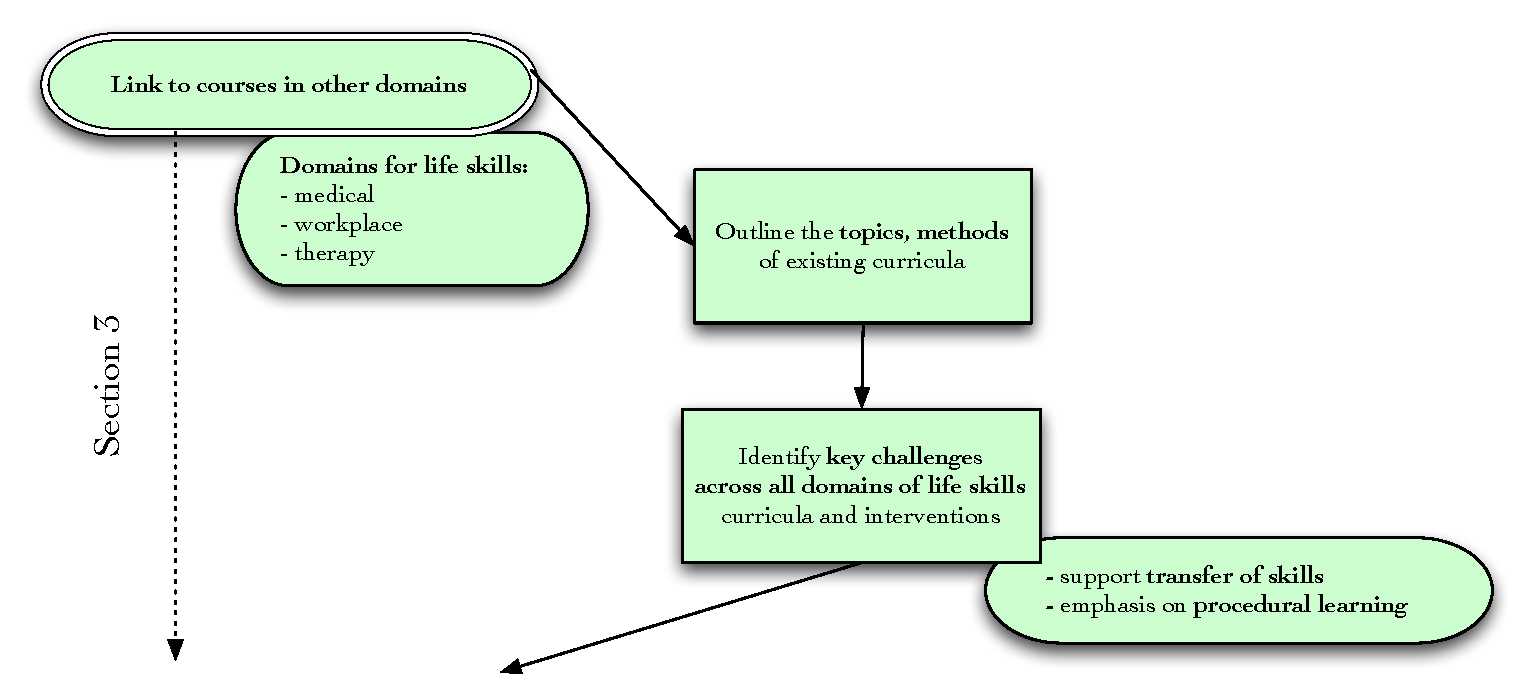
\includegraphics[scale=0.5]{imagess/JournalStructure3.pdf}
%       \caption{Overview of Section~\ref{sec:linkDomains}}
%       \label{fig:linkDomains}
%\end{figure}
  


%\vfill ~ \pagebreak
% \rephrase{These fit well to the 5 core values identified for SEL} 

% {{{ Therapy 
\subsection{Talk-based therapeutic settings}
A crucial part of talk-based psychotherapy aims to support the development of social and life skills, often for clients  disadvantaged by cognitive or emotional deficits or going through difficult life situations at the time. % mainly for clients  with cognitive or other deficits.
%
The literature in this domain focuses on two main aspects. First is the psychotherapy itself, i.e., strategies to support learning and improvement on the part of the clients. The second aspect concerns the training and development of the skills needed by the therapists/counsellors themselves, with the emphasis on supporting the learning process for the trainees leading to sophisticated combinations of class based learning and practice with real clients (under supervision of an experienced therapist). 



\subsubsection*{Methods}  
The methods used to work with clients during the therapeutic process differ depending on the psychotherapy approach chosen by the therapist. These can range from very specific training situations and exercises such as exposure therapy in Cognitive Behavioural Therapies (CBT) or social skills training for people with autism, to unstructured exploration of personal experience in humanistic approaches.  See, e.g., \citeN{Coyle2007} for a succinct review of the most common psychotherapy schools and links to further resources; and \cite{Kientz2013} for an in-depth review of technologies developed to support autism therapy. 
%
Skills development for students and novice therapists builds on a mix of lectures on the theoretical background and how to put these into practice. This is done initially with peer students who role-play clients and share and discuss their (real) problems; later in the learning process this also involves real-clients, where the students lead the psychotherapy under close supervision of an experienced therapist. The emphasis on supervision is high, with the majority of schools/colleges requiring student therapists to enroll into psychotherapy for themselves while studying. 


\subsubsection*{Topics} 
In terms of supporting the client directly in the psychotherapy process, the topics differ substantially depending on the clients' issues or disorder, and personalisation is crucial. As such therapies can, for example, aim to help clients to achieve better self-awareness, to develop better  self-control, decision making processes, and interpersonal skills, and to help change deeply set negative thinking patterns.  %For a more specific example, clients with autism often have difficulties with basic social skills such as understanding emotional states of others or engaging/disengaging from interactions.  
% also examples from Coyle2011? -- depression, anxiety management
%\todo{add something on the effect of providing client feedback as a novel approach? }
%
Therapist training is most concerned with very detailed self-awareness on the part of the therapist, and mastering the techniques and approaches of the studied psychotherapy approach. The ability to empathise and fully listen to the clients is particularly emphasised as a key therapeutic skill. The aim of all these social and emotional skills is to help develop a good working relationship with clients, which is seen as one of the main aspects of successful psychotherapy \cite{Asay1999}.

\subsubsection*{Reviews}
Therapeutic settings have already generated considerable research within
HCI,  looking at using technology to extend and improve the psychotherapy process. The work so far focused mostly on autism related systems (e.g.,
\cite{Escobedo2012,Picard2009,Hayes2011,Porayska-Pomsta2011,Hong2012} and many others), and cognitive-behavioural therapies (e.g., \cite{Coyle2011,Matthews2011}). \citeN{Coyle2007} in particular gives an overview of the use of technology in psychotherapy, the potential for HCI involvement, and a solid introduction to most common psychotherapy styles.          
%
In addition, \citeN{Hill2006} review existing literature on teaching counselling and psychotherapy students, showing significant positive effects of particular training methods. The book edited by \citeN{Duncan2010} provides a detailed review of the factors common across various therapeutic approaches, including the large positive effect sizes of most therapies, and the key role of the therapeutic relationship. 

%\citeN{Vismara2010} reviews another for empathy as key for therapeutic process (maybe something from Marci + can use the Heart of therapy book)
%\item also reviews on the efficiency of therapy (maybe Coyle2007 has some?)
%\end{itemize}




%\Geraldine{ G: include as sub-section of clinical setting? also use some [pubsense seed paper refs] to motivate effectiveness of empathy in this relationship?}
%\begin{itemize}
%       \item .... not sure how much space this should get, given it has been already %addressed in earlier work. Although, I guess that this could also point to a slightly %different approaches than those used at the moment? 
%       \item Probably need to emphasise that each and every competency can be addressed, %depending on the therapy style/clients issues.
%       \item A short paragraph with link to David's review for specific work done in HCI. %Plus a few sentences linking the way how students become therapists, through again %role play, a lot of practice etc. Have a decent link for this \cite{Hill2007}, but %will ask Stef in Nottingham for others.
%       \item Also links to autism literature for additional examples?.
%\end{itemize}  
% }}}

% {{{ Medical settings
\subsection{Medical settings}
\GeraldineFIX{ G: need to think about this TITLE bit more - is this meant to be medical as in just doctors, or medical in its broader sense? Eg doctors, nurses, allied health, therapists, etc ... in which case 'clinical settings' might be a more encompassing term.... }
\GeraldineFIX{ G: then in writing up. you can say you focus first on the medical profession ... and do the doctor-patient training .... and then look at other healthcare/clinical professions more generally eg including nurses, physios, counsellers/therapists etc???}
\GeraldineFIX{ G: Also think the section structure could be thought about a bit more ... eg is it useful to separate out different SEL foci:... \\
1. being a better dr and managing own HWB (eg mindfulness skills); \\
2. general clinican-patient relationship eg.\\
gathering information from patient (interview/question skills???); giving difficult news;  establishing collaboratively designed care plans, empowering patients to take own responsibility etc ... there is a term for this model fo care but can't remember! (eg as in motivational interviewing)}

Social skills, such as communication skills and empathy, are increasingly recognised as core clinical skills in the medical community \cite{Rider2006,Barth2011,Makoul2007,Kalet2004}. Improvements in such skills have been shown to enhance patient satisfaction, increase adherence to therapy, and promote patient willingness to divulge sensitive information that may assist diagnosis as well as reduce the risk of subsequent litigations \cite{Stewart1995,Brown2008}. %As Brown \cite{Brown2008} puts it,  ``Over the last 20 years, the topic has raised from its status as a "nice to know" subject to that of a "need to know" skill set in modern medical education''. 
Most curricula focus on one of  three areas: (i) university courses for medical students; (ii) general courses and support for practising medical personnel; and (iii) specialised courses for specific groups of medical personnel, such as in cancer care or end-of-life care, where specific skills related to empathy and communication are even more important        (e.g., when giving bad news to patient). Most of the courses are available for doctors, with courses also offered for nurses and other health professionals. Peer-reviewed evidence exists for the effectiveness of  many of the interventions in this domain for improving the targeted skills
(see reviews below).
% also physios (who do a lot of motivational interviewing to help people develop rehab programs they can stick with etc)
% reference Yedidia2003 -- intervention for students 

\subsubsection*{Methods} A popular method in medical settings is the use of role play both with peers and using trained actors  \cite{Stepien2006,Stiefel2010,Kalet2004,Barth2011}, as well as facilitator or peer based feedback \cite{Rao2007}. 
\GeraldineFIX{G: \textbf{(G: on what?\ on the role plays, or is this another method ie not clear what 'followed by' refers to ... popularity or how role play is used)}}
Courses also include workshops, lectures, and discussions of case studies. Many courses that aim at general communication skills include role plays with scripted exchanges or examples to practise on. 
 \textbf{\GeraldineFIX{G: (G:\ how are these different to role plays??) P: These a specific sub-part of role plays (i.e., you can have other role plays without scripted exchange). I believe it is worth mentioning as such scripted (iu.e., fixed) exchanges can be readily supported by technology.}}


\subsubsection*{Topics} 
Curricula focus both on self-oriented emotional skills for medical personnel as well as a wide range of interpersonal interaction skills. 
%
Courses on self-oriented emotional skills include aspects such as personal reflection, self-awareness mindfulness, and stress management training \cite{Shapiro2000,Epstein1999,Satterfield2007}. This also incorporates the growing emphasis on the importance of teaching medical students and healthcare practitioners to manage their own well being, for example through teaching mindfulness techniques and lifestyle management \cite{Hassed2009}.
%
Courses on interpersonal skills aim to support generic patient-clinician interaction. The emphasis is on the ability to inquire for diagnosis related information and to clearly communicate test results and offer  treatment suggestions (e.g., see \cite{Kalet2004,Barth2011} for examples and review); related techniques, such as  motivational interviewing \cite{Miller2002},  focus on skilful framing of questions with the aim of empowering  clients to take responsibility for their own behaviours and decisions.  
\GeraldineFIXNEW{GF NOTE: Hettema is not a classic motivational interviewing ref - some Miller ref is better to use here eg Miller, W. R., \& Rollnick, S. (1991). Motivational interviewing: Preparing people for change. New York: Guilford Press. OR Rollnick, S., \& Miller, W.R. (1995). What is motivational interviewing? Behavioural and Cognitive Psychotherapy, 23, 325-334.}
%
 
Empathy is understood as another crucial component of successful and caring interactions between the patient and doctors, nurses and other health professionals. Empathy is particularly important in interactions communicating deeply emotional and life-changing information, e.g., in oncology, and to a lesser extent also in other general practice \cite{Barth2011}.
                For example, doctors often tend to ignore patients' emotions during difficult moments (e.g., having to communicate a critical diagnosis) and concentrate on the pragmatics, leading to negative consequences for treatment adherence and psychological functioning of patients. The training involves aspects such as sensitive responding to emotions from patients and improved understanding of the patients' psychosocial issues, concerns and needs as well as methods to do so while protecting the emotional well-being of the clinician or nurse. 


\GeraldineFIX{ G: say what technology how used in a sentence???}
\GeraldineFIX{ G: this doesn't seem to be empathy but about self awareness/regulation?  ... P: Is this a bit better? 
I'm drawing on the reviews and the concerns they use in this space -- in my reading it is also around objectification of the patient etc... where regulation is obviously important, but also as a part of being able to emphasise in these cases without burn-out etc. .. I think it might be too complex to go into details here (especially given what a tangled mess empathy as a concept is :)}
        %       \item Additional focus on specific communication skills  such as breaking bad news for oncologists and \todo{...}.

\subsubsection*{Reviews} \citeN{Rao2007} present a systematic review of interventions designed to enhance communication behaviours between patients and doctors, and \citeN{Barth2011} systematically review communication courses specialised for oncology personnel (e.g., doctors, nurses, social workers). Both  found statistically significant positive effects of skills training, such as improvements in patient-centered communication skills as well as higher ratings from the patients. Emotional skills training for medical students is reviewed by \cite{Satterfield2007} and shows positive effects of the interventions. \citeN{Pedersen2009} and \citeN{Stepien2006} review training courses that specifically aim to increase empathetic skills of students or practitioners. There have also been some successful initial studies
on including technology into the teaching process, e.g., \citeN{Tulsky2011}
shows the benefits of combining lectures with tailored video-recording of
the doctors' own interactions for later reflection.

% }}}

% {{{ Workplace and business relate
\subsection{Workplace and business related settings}

A focus on emotional and social skills teaching also has a long history in the workplace, e.g.,  \cite{Bailey1983,Bailey1983a}, appearing under a wide range of labels such as interpersonal skills, soft-skills or, more recently, emotional intelligence and developmental workplace coaching. Social and emotional skills training is included as part of professional educational programmes such as for MBA and undergraduate business students; it is also offered as part of ongoing professional development in the workplace, e.g., many companies offer soft-skills courses or coaching to their executives and increasingly also to other staff. 
%
Academic literature shows positive effects of such training (such as improved leadership, team-building or self-management skills),
\GeraldineFIX{G: \textbf{(G:\ SUCH\ AS???)},} 
but the existing evidence is not as strong as for SEL in education. Some of the reasons are that training programs have often been developed on a purely commercial basis and outside of the academic community  and detailed information about the content of the programs is often not available for intellectual property and/or competitive advantage reasons \cite{Walter2011,Clarke2006,Riggio2003}. 




\subsubsection*{Methods} The majority of courses follows similar strategies: role-play as a key approach to teaching the skills, together with discussion of fictional and real life cases, demonstrations and modeling. The emphasis is again placed on procedural learning and the opportunity to practise and embed skills so that they become automated. Time-frames differ from a few hours to multi-day courses, and to longer-term learning relationships (e.g., as in coaching). 

\subsubsection*{Topics} 
        A key focus is on developing aspects of emotional intelligence (EI), which can be defined as ``the ability to carry out accurate reasoning focused on emotions and the ability to use emotions and emotional knowledge to enhance thought'' \cite{Mayer2008}. Such training might, for example, develop communication and cooperation skills, as well as increase self-awareness of the employees. 
%        
        Specific leadership programs focussing on SEL skills in the workplace designed for executives are often aimed at relationship skills (such as conflict management and interviewing) and self-management (e.g., dealing with stress or time-planning and goal setting). Executives are often expected not only to learn these skills themselves, but also to be able to teach them to others later on. Coaching is often used as a way to help executives (and increasingly other employees) develop EI skills \cite{Bono2009}. It is inherently client-focussed, with the goals agreed depending on the situation, and emphasises accountability to the coaching relationship, honest feedback, supported reflection and accepting responsibility for own decisions. 

\GeraldineFIX{G: Not just for executives though in the workplace - this can sound like it is only for execs?    P: That's what the reviews I found focused on ... perhaps still mainly used for execs, as very expensive to roll-out more widely? Or perhaps not that much literature on it?}

\subsubsection*{Reviews}  \citeN{ArthurWinfred2003} provides a general overview of the effectiveness of training within organisations, including training of interpersonal skills, and discusses the effects of various training designs. Their meta analysis reveals medium to large positive effect sizes  ($d$ around $0.60$) for organisational training courses. \citeN{Mayer2008} gives a thorough review of the 'emotional intelligence' concept, including connections between emotional intelligence and better real-world performance.   \citeN{Feldman2005} and \citeN{Bono2009} summarise the practices and processes used in executive coaching by practitioners, and \citeN{Carey2011} provides a rigorous review of academic literature on work-place based coaching for leadership. \GeraldineFIX{G: ??? seeing you also mention coaching under the personal area?? ... P: But this review really does talk about work-place only, with particular focus on leadership}
% }}}

% {{{ Mindfulness
\subsection{Everyday life skills}
Everyday life skills courses comprise a wide range of fragmented topics and methods. As such, we only briefly point to several illustrative examples where social and emotional intelligence skills are taught in, and for, everyday life settings. These are often framed as  various life skills courses  for the general population such as interventions supporting interpersonal skills (e.g., improving empathy for couples \cite{Long1999,Angera2006}) or interventions based on meditation, yoga, and more recently Mindfulness Based Stress Reduction \cite{Kabat-Zinn2003}, all aiming to support and improve personal well-being (e.g., \cite{Grossman2004,Marchand2012}).  %.  -- couldn't find any literature on courses that would not be for medically relevant population. My guess is that they exist (as per many such courses in the universities), but I have no reference to point to, yet. I also did not find an overarching review of mindfulness courses, closest available is \cite{Ludwig2008}. 
Moreover, the growth of life coaching (e.g., \cite{Green2006})  and consultation services, most commercially based, as well as the wide usage of self-help books, point to the increased recognition by people of the value of positive self-driven change and interpersonal and emotional regulation skills. 
%
Altogether, these examples draw out the large scope of everyday life skills learning, and the value people place on them.

\GeraldineFIXNEW{PETR --- I don't have any examples of out-of-HCI emotional regulation courses for general populations. I'm sure they exist, but didn't get to see any yet. We also reference the HCI stress related work in Section 3. 
GF NOTE: should you be saying a little more about stress here as a current trendy focus ... especially seeing the MSR work there? Think I also forwarded on a coaching paper in the last coule of days that might be relevant - yell if i didn't}

\GeraldineTODO{G: (G: add a little more on life coaching since a growing area? example refs in comments - chapter mentions some reviews but says more needed of course  P: I have a psychology of coaching book at home -- I will have a look if anything can be pulled out from there)  P: Plus read the Green2006 paper in more detail}
% http://books.google.at/books?hl=en&lr=&id=MkVBx4n5Y6EC&oi=fnd&pg=PA125&ots=WatB-ZtV4x&sig=edfjCOfMf5v3krOh3dHJ5SCauDo#v=onepage&q&f=false
% http://www.tandfonline.com/doi/abs/10.1080/17439760600619849#.UfuPPlNRsW4
% http://books.google.at/books?hl=en&lr=&id=kFiizfiMyjYC&oi=fnd&pg=PR7&dq=personal+coaching&ots=h33TQQvGzC&sig=-F85hpID5QHlTqcuuMKnrybXGs0#v=onepage&q=personal%20coaching&f=false
% http://www.psychotherapy.com.au/shop/book-store/therapeutic-approach/psychology/the-handbook-of-coaching-psychology.html
 


%\subsubsection*{Methods}  
%\subsubsection*{Topics} 
%\subsubsection*{Reviews}

% }}}



%}}}

% {{{ SECTION: Conclusions
\section{Conclusions}
\label{sec:conclusion}

This paper points to the potential of mutual cooperation between HCI and social and emotional skills learning (SEL), benefiting both disciplines.
%
We outlined the key challenges for current SEL approaches, including the lack of support for transfer and 'embedding' of skills from the SEL lessons into students' interaction, encouraging parental involvement, as well as enhancing the support for development of reflective abilities and novel environments for practice. 
%
The review of existing HCI research shows there are strong indications that technology could help address many of these challenges. We drew on existing HCI work in a wide range of areas such as ubiquitous computing, emotional awareness and reflection, sensor-based tracking, social networks, design, and (serious) games. As such, HCI involvement in this space has the potential for for strong, real-world impacts, especially given the wide (and ever increasing) penetration of SEL programs in our schools, workplaces and everyday life.  
%
We also highlighted how the focus on SEL provides new challenges for HCI, as well as a structure to further guide and support HCI research around social and emotional interactions -- both as a 'test-bed' to develop cutting-edge technology in, but also as a 'knowledge base' we can build and learn from as we shape this emerging research area for HCI. 
%
Overall, this paper suggests that social and emotional learning points to a novel, complex, intriguing research space, which has a high potential to enrich HCI research and practice.




%In doing so we have presented a set of structured concepts and characterisations of SEL to help frame an agenda for further research. We provide a summary of the topics, methods, and learning principles, and their associated challenges in SEL across the domains (Table~\ref{fig:SummaryResults}); we review HCI research relevant to the respective challenges (Table~\ref{fig:HCIsummary}) and outline the design space and opportunities for HCI  (Table~\ref{tab:session6summary}).



%



%




%We end by highlighting three selected aspects of SEL we personally find particularly interesting for immediate future work within HCI. These are (i) addressing the support for social and emotional learning in education of neuro-typical children (a domain with a long history, many curricula that are widely applied, but so far under-researched in HCI); (ii) the implications of supporting facilitated learning in SEL (and the differences in design settings it brings); and (iii) finding ways to mesh HCI research and technology support well with the curricula design (building on the long history of research there).
%       \todo{what this means for HCI}
%       \begin{itemize}
                % build on the special needs research to look at neurotypical groups
                % Focus on facilitated learning and the design implications it has -- in-class learning as an important settings to start from, and supporting out-of-class, ``in the wild'' learning as a way to address the key challenge.
%
%       \end{itemize}



%
%The distinction and characterisations we offered here are likely to be only an initial attempt to describe the nuances of the field.
%It is our hope that while the characterisations and distinctions suggested in this paper could be useful for immediate future work into this space, further research will elaborate on, clarify and extend, rather than reify, these.


%\todo{something feels wrong -- maybe not well balanced and/or missing the extent of research into autism (and other special interest groups?)}

% }}} 

\bibliographystyle{acmsmall}
\bibliography{library}

\bigskip

\section*{Authors' statement}
This work is not, and has not been, submitted for a review in any other venue. No part of this work was previously published or has any direct relationship to our existing/submitted papers. 
\end{document}


%%%%%%%%%%%%%%%%%%%%%%%%%%%%%%%%%%%%%%%%%%%%%%%%%%%%%%%%%%%%%%%%%%%%%%%%%%%%%%%%%%%%%%%%%%%%%%%%%%%%%%%%%%%%%%%%%%%%%%%%%%%%%%%%%%%%%%%%%%%%%%%%%%%%%%%%%%%%%%%%%%%%%%%%%%%%%%%%%%%%%%%%%%%%%%%%%%%%%%%%%%%%%%%%%%%%%%%%%%%%%%%%%%%%%%%%%%%%%%%%%%%%%%%%%%%%%%%%%%%%%%%%%%%%%%%%%%%%%%%%%%%%%%%%%%%%%%%%%%%%%%%%%%%%%%%%%%%%%%%%%%%%%%%%%%%%%%%%%%%%%%%%%   FINISHED %%%%%%%%%%%%%%%%%%%%%%%%%%%%%%%%%%%%%
%%%%%%%%%%%%%%%%%%%%%%%%%%%%%%%%%%%%%%%%%%%%%%%%%%%%%%%%%%%%%%%%%%%%%%%%%%%%%%%%%%%%%%%%%%%%%%%%%%%%%%%%%%%%%%%%%%%%%%%%%%%%%%%%%%%%%%%%%%%%%%%%%%%%%%%%%%%%%%%%%%%%%%%%%%%%%%%%%%%%%%%%%%%%%%%%%%%%%%%%%%%%%%%%%%%%%%%%%%%%%%%%%%%%%%%%%%%%%%%%%%%%%%%%%%%%%%%%%%%%%%%%%%%%%%%%%%%%%%%%%%%%%%%%%%%%%%%%%%%%%%%%%%%%%%%%%%%%%%%%%%%%%%%%%%%%%%%%%%%%%%%%%





\iffalse
% {{{ OLD SECTION --- Chp 5
% {{{ OLD text
\iffalse
\vfill ~ \pagebreak
This section draws out the potential synergies between the social and emotional learning, and existing HCI work and interests. We use the four learning principles to orient the discussion as they provide a direct connection to the curricula structure and approaches, and also to illustrate how this differentiation can serve as a good initial basis to guide thinking about  future HCI work on this topic. 

As an overview,  Table \ref{fig:HCIsummary} outlines the broad connections between the learning principles, relevant themes of research in HCI, and exemplary areas particularly suitable for technology support. We address each learning principle separately, with illustrative examples of relevant HCI work. These examples suggest the extent of existing HCI research that could be re-appropriated as relevant to social and emotional learning and also highlight the opportunities and challenges this would pose to HCI research. We end by drawing out some of the roles technology could take across the learning principles. 


\begin{table}
  \centering
        \includegraphics[width=\textwidth]{images/SummaryHCI.pdf}
        \caption{Depiction of relations between the learning  principles, the links to HCI, and the related broader topics in HCI research}
        \label{fig:HCIsummary}
\end{table}
\GeraldineFIX{ G: subtopics for feedback - reflect all of topics from earlier?; add 'scaffodling practise in class under practice subtopics?}
\fi
% }}}


% {{{ Embedding into every day  
\subsection{Embedding learned skills into everyday life} 
\todo{ADD SEL EXAMPLES FOR EACH POINT!}

Once a skill is partially learned, for example when the learner can enact it in a simulated situation within the class, the ultimate goal of the curricula is to support the learners in embedding such skills into their everyday behaviours and situations. In other words, embedding aims to support the transfer of skills learned in facilitated sessions into skills that are increasingly generalised and ingrained into everyday situations. In this sense, there is a subtle but important difference between embedding (background support for on-going, natural, everyday situations, over longer periods) and practice (a consciously enacted, specific activity aimed at practising a particular skill).

Despite its importance, there is little trainers (or curricula designers) can do to facilitate and support such embedding at the moment. %apart from in-sessions training (e.g., role-play with real-world examples or dealing with naturally arising situations), or attempts to increase awareness awareness of the learned concepts outside of the sessions by, e.g., posters, reminder emails and, in the case of SEL for education, letters to parents.
%
In the rest of this section, we outline two exemplary ways in which existing HCI research might help address the challenge. First, a large body of research exists on using technology to facilitate behavioural change, supporting people in changing their everyday activities and habits. As social and emotional skills are also mostly behaviours (rather than, e.g., declarative `knowledge'), many of the techniques introduced in HCI to promote behaviour change for health or ecological sustainability are likely to be relevant for SEL.\GeraldineTODO{G:  although the specifics of social skills again have the potential to further challenge existing HCI systems into novel directions ... why, how? be a little specific here? } Second,  technology can tap into social support for embedding skills in everyday life. For example, technology can be used to share part of the expert/trainer role to other social contacts in the participants' lives, such as drawing on social support and feedback from their friends, colleagues, and parents (in the case of SEL in education); as well as to support interactions with online networks (who may be strangers but who  share the same goals). 
%
Together, such use of technology has the potential to enhance and augment one of the greatest challenges of the existing social and emotional skills learning curricula. 


%\todo{The earlier text is just about social support. Now we want to start with making skills habitual etc. as per the text copied below from the intro:}

%\todo{Old text:} Throughout the social skills learning process, the provision of support  from parents and family during everyday life is key for many of the analysed curricula. This kind of social support can provide a potential way of integrating the learning into everyday life. However, such embedding in everyday life is, in some ways, the least developed aspect of the curricula, currently  mainly done by meeting with parents at the beginning/end of a course and by sending letters and asking school children to do homework. In this area, technology can be employed in two ways: One the one hand, to facilitate social support by utilizing situated systems which connect students with their family and peers; and on the other hand by using ambient and ubiquitous persuasion that can sense student's activities in context and give adequate and timely feedback also outside the classroom.

% {{{ Behav change
                \subsubsection{Behaviour change technologies}
Learning new social and emotional skills often includes a considerable change in habits and ways learners would automatically react and/or behave; this is also one of the key reasons why procedural learning is emphasised across all curricula and domains. %Routines and habits as something to be changed -- similar to social skills where although motivation for change might be present, hard to change existing patterns. 
As already noted, while techniques for procedural learning are well established and available within sessions, curricula currently have few options to support embedding of the skills into everyday patterns of behaviour of the learners.

        
Behavioural change research within HCI has dealt with similar challenges, mainly in the context of health and ecological sustainability \cite{Hekler2013,Consolvo2009,Klasnja2011,Fitzpatrick2009}. % Such systems are often based on helping participants increase/reduce particular activities (such as go running, or stop smoking), often by facilitating that neccesary behaviours become a part of users daily schedules (e.g., running at least 3 times a week, or not having more than 1 cigaret a week), thus shaping new habits.
Many behavioural change systems are based on pervasive technology used to track user behaviors in everyday life over extended time periods, and to help facilitate users' reflection and discovery of emerging patterns, enable exploration, and monitor own progress. For example, usage patterns of electricity \cite{Gustafsson2005}, water \cite{Kuznetsov2010} and food \cite{Ganglbauer2013} have been tracked and displayed to users to encourage conserving these resources.  Similarly, mobile devices and sensors have been used to continuously track personal information such as physical activity data  \cite{Lin2006a,Consolvo2008a} to facilitate ongoing awareness and promote healthier lifestyle habits; mobile devices have also been used to  help participants manage domestic activities such as TV consumption and household chores \cite{Reitberger2013}, fostering reflection and renegotiation of such activities based on awareness of behaviour patterns over time.
%

Although behaviour change literature directly addressing social skills is scarce in HCI so far, we expect that  similar strategies and technologies we see in other behavioural change topics could work well also for (parts of) SEL.
%despite clear differences in what types of activities are tracked or supported, and the technical difficulties for doing so  (e.g., social skills being harder to measure when compared to tracking the water consumed or distance ran).
Several examples of existing work provide preliminary evidence on how such long-term support and embedding might be possible. %, perhaps through higher reliance on the capabilities and reflection of the users.} 
%
%One such example is SocialMirror \cite{Hong2012}, \Geraldine{G: Hong is repeated here and below on the same page - use hte example just once or be clearer about different emphasis - currently sounds too similar and repeats }an ambient system to support embedding of learnt everyday behaviours of people with autism who are living independently, allowing the users to ask and receive feedback\GeraldineFIX{G: not so clearly behaviour change in the way it is described? } from a trusted community of acquaintances and professionals;  and 
In one such example, \citeN{Munson2010} integrated a well-known positive psychology intervention into a social networking site, meshing with users' daily habits around these sites. 
Similarly, \citeN{Mamykina2008} designed MAHI, a system for newly diagnosed diabetes patients, extending the in-class lessons by facilitating participants' ability to track, reflect on and analyse their everyday experiences with diabetes, leading to improved feeling of control over the disease.
%\GeraldineTODO{G: again not so clearly behaviour change but better fitting with reflection section???}

Altogether, the examples above suggest that many behavior change techniques have potential to foster the continuous application of learned skills throughout everyday life, and support learners in sustained and habitual use of these skills in the appropriate situations. %However, major challenges remain for HCI in this area, such as the robust sensing of social skills and interactions, adequate feedback modalities and finding the right duration and frequency for the deployment of the respective technologies.   
% }}}

% }}}

% {{{ Engagement and motivation
\subsection{Engagement and motivation}

Facilitating engagement and supporting motivation of the learners is important across all domains and curricula. %but could be improved upon? current curricula, espec. 
%
%, and cuts across activities in the other learning principles. %While educational domain curricula often include aspects aiming to engage learners, such as stories or animated characters children can identify with, specific focus  % , while the other domains not as much, despite the key importance. 
A large body of work in HCI focuses on creating engaging experiences, showing the potential of technology and design to enhance users' engagement with a wide range of aspects, activities and concepts such as school education \cite{Connolly2012,Bers2010}, digital art \cite{Edmonds2013}, or stroke rehabilitation \cite{Balaam2011a} to name just a few. This breadth of topics, as further illustrated, e.g., in the Funology book \cite{blythe2004funology} and subsequent research, suggests the high potential of similar approaches to augment many aspects across the curricula, making social and emotional skills learning more engaging and motivating.

Similarly, the recent uptake of systems that aim to support users' engagement through 'gamification' or 'gameful design' \cite{Deterding2011,McGonigal2011} \GeraldineFIX{G: have to be careful about who we claim as HCI eg don't imagine mcgonigal would label herself as hci  \\P: is this ok now? I don't think we are claiming it to be HCI ... the newly added 'similarly' maybe can help emphasise this?}could be particularly relevant to social and emotional skills curricula,  integrating game mechanics like rewards, goals, points or challenges into real life activities.  
%
%\todo{pull out very specific examples, then link back to behavioural change and its motivational aspects -- or rather say this is something behave change draws on as well?}
For example, Superbetter\footnote{\url{http://www.superbetter.com/}} aims to help players increase their personal resilience, using a structure of quests, adversaries, and power-ups to engage players with scientifically endorsed exercises. Other applications in this area are related to behaviour change technologies, such as supporting users to become more fit (e.g. via activity tracking sensors coupled with gamified services such as Nike+ and Fitbit), lose weight  (Withings) or to improve people's sleep (Zeo). 
%
Gamification approaches have been also successfully applied in education (e.g., \cite{torres2011quest,Sheldon2011,Mamykina2008}), as well as psychotherapy work \cite{Goh2008,Piper2006}. %\cite{Liu2010} to support English learning, not only leading to increased motivation but also to improved outcomes when compared to a conventional learning setting. 
Several game-based systems looking at social skills with children also report positive effects and high engagement of the users, e.g., \cite{Hourcade2013,Hendrix2009a}.

All of these examples highlight the possibility of technology based systems to create intrinsically motivating applications that draw user in and are fun to interact with, regardless of the activity or behaviour to be supported. 
\GeraldineTODO{G: just wondered about also including some references to increasing principled work looking at how to interpret theories of motivation in systems and developing design strategies .. so SEL\ can also build on this growing understanding eg Consolvo et al 09 (see comment)  }

\GeraldineTODO{G: also wonder about for somewhere in section 5:\\ - pointing to/naming work on personal informatics for self reflection etc somewhere in section 5 eg li et al 12;\\  -  pointing to ESM\ work as a way of getting people to capture records in situ\\ }
% http://dl.acm.org/citation.cfm?id=2212724&CFID=348098226&CFTOKEN=10085713



% }}}
% }}}

% {{{ Summary -- chp5

\subsection{Summarising technology roles across learning principles}    

Across all of these examples, we see a range of successfully deployed---or potentially deployable---HCI systems. While the presentation was so far structured according to the learning principles (showing HCI can address the key challenges), we can also see across the presented examples broad categories of types of technologies that can be deployed to support different principles. We draw out some of these categories here to illustrate the general classes of technologies that can support SEL. This variety also points to the complexity of the design space and emphasises that supporting a particular learning principle does not necessarily prescribe a particular role for, or type of, technology.

%We now discus according to the similarities in the role technology plays there rather than the learning principles they support:   %\rephrase{A rough distinction of the benefits offered by technology that appeared repeatedly could be to distinguish:}
        \begin{enumerate}
                \item {\bf Expert sensing:} Some of the systems rely on sensing and automated interpretation of behaviour, helping users draw out patterns they were not aware of before. Information can be presented in real-time, such as giving feedback on communication behaviour in meetings \cite{Kim2008,DiMicco2007}, or over longer periods of time such as in AffectAura \cite{McDuff2012}. Such systems often draw on and connect many disparate data sources. 
                
                %\todo{this is future?} taking over some of the feedback from the trainers/peers or giving additional one (\cite{fjklds,fds,fsd,fsd,sdf}). 


                \item {\bf Structuring activities:} Other systems aim to provide timely reminders to support users behaviour. They may provide data for the user to reflect and act on, but rely much less on automatic sensing and interpretative capabilities of technology, leaving the interpretation to the user. Examples can be found in autism technology such as MOSOCO system \cite{Escobedo2012} listing the appropriate actions the person should take and asking them to rate their performance (i.e., no sensing on the part of the system); personal reflection tools, such as Affect Diary \cite{Stahl2008} and systems around SenseCam (e.g., \cite{Fleck2009}; or facilitating keeping of diaries in psychotherapy \cite{Matthews2011}.  

                \item {\bf Novel experiences:} A third role we saw systems take was to facilitate or create novel experiences. This can be either by providing a 'new world' to behave in,  as per (serious) games \cite{Hailpern2011} and virtual reality \cite{Bouchard2012,Romano2005};  or by helping the users to get a novel perception of a particular behaviour such as through gamification of real-world experience (e.g., Superbetter app) and  the accentuated feedback in systems developed by \citeN{Bailenson2008}. 

                \item {\bf Connecting and sharing:} Fourth role was in supporting connecting and sharing among larger groups of users. For example, facilitating cooperation by reaching out to social support nets (e.g., \cite{Newman2011}), or the family/friends circle (e.g., \cite{Hong2012,Munson2010}).


\GeraldineDIS{G: need to include displays/modalities or whatever here too?   P: It doesn't seem to fit for me here, but perhaps I just misunderstood. The rest of the section talks about {\bf what} the technology does (conceptually), while modalities/displays are rather about specific {\bf hows} to do thigs like this. As such, they then got grouped into the design challenges.}        
\end{enumerate}

%\todo{The first two maybe don't work -- mixing together 'patterns over time' and 'making invisible visible', no clear distinction otherwise -- apart from the expert/non-expert approach. Do we combine these together then?}
        
 

%\subsection{Summary}
%\todo{(in a state of utter rubbish now:)}
%The previous sections unpacked the learning  principles identified earlier, linking them to existing work within HCI and pointing out how such \rephrase{combination} might be especially useful for both SEL, by providing novel opportunities to teach and learn social skills, as well as for HCI through \rephrase{interacting} with an interesting new domain for which useful applications can be developed and, by doing so, challenge and inspire further research within HCI.  


%The Figure~\ref{fig:HCIsummary} shows a summary of this, including a list of more general topics within HCI for challenge, from which we drew the examples mentioned in sections above. \todo{It is still a very rough draft of the figure -- not sure if it makes sense, and what "buzzwords" from HCI should be used in the end for each challenge. Still, the goal is to somehow tie the examples showed before in a more simplistic way to the research within HCI, and also indicate that it could be relevant to fairly large crowd.}

% }}}


% {{{ SECTION: Future research agenda

\section{Mapping out the design space -- opportunities and challenges for HCI}
\label{sec:agenda}
  

Previous sections have so far looked at what social skills curricula focus on and where the challenges lie (sec 2-4);  and then provided examples showing how these challenges and learning principles could be supported by technology (sec 5).  While drawing out some of the HCI research that is already very relevant to these domains, section 5 was however still structured by the learning principles and social skills learning challenges, aiming to show that HCI has the potential to address many of the key issues there. 

In this section we take a different viewpoint and outline the challenges (and thus also opportunities) that supporting social and emotional skills curricula would pose to HCI, across the learning principles and curricular domains. We focus on four main areas, outlined below and in Table~\ref{tab:session6summary}:


\begin{table}
  \centering
        %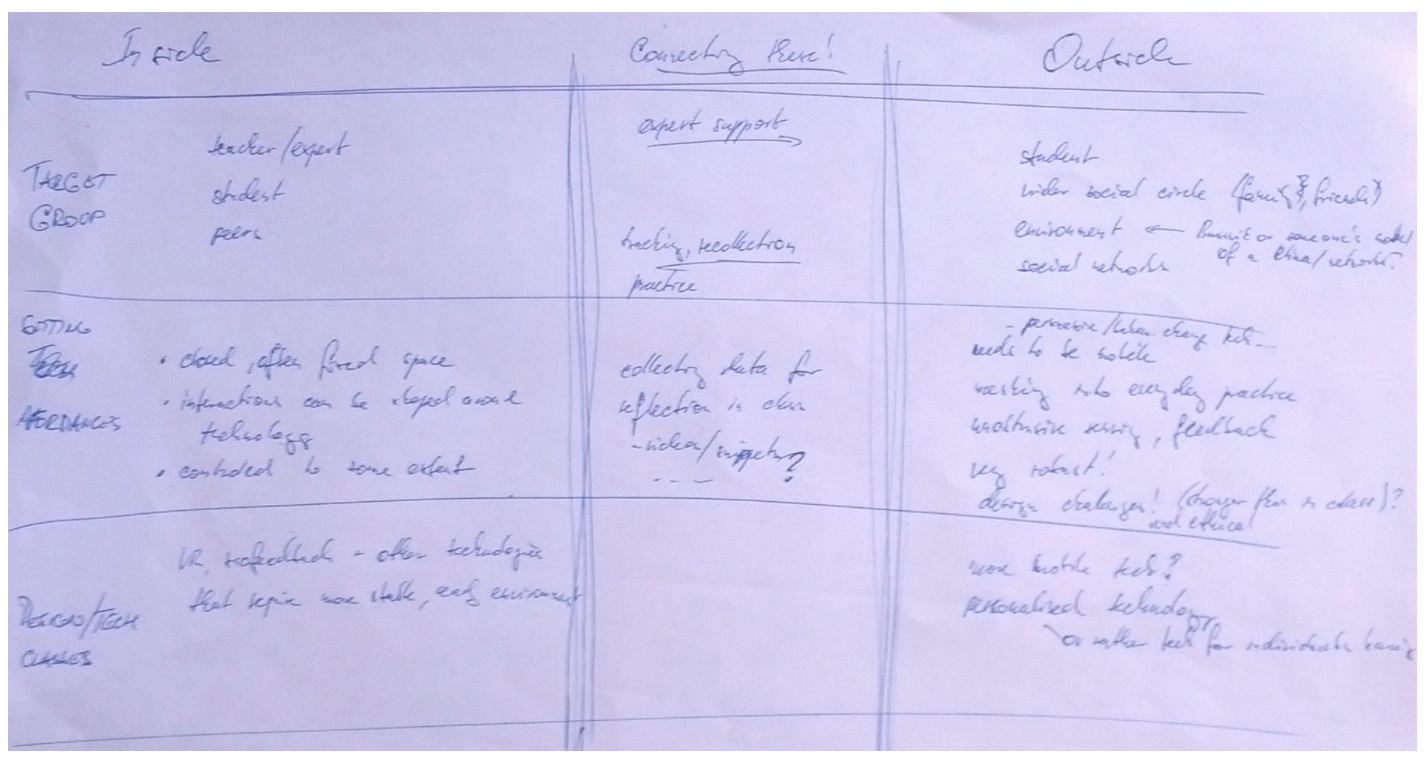
\includegraphics[width=0.8\textwidth]{images/In-out-sessionDimensions.png}
        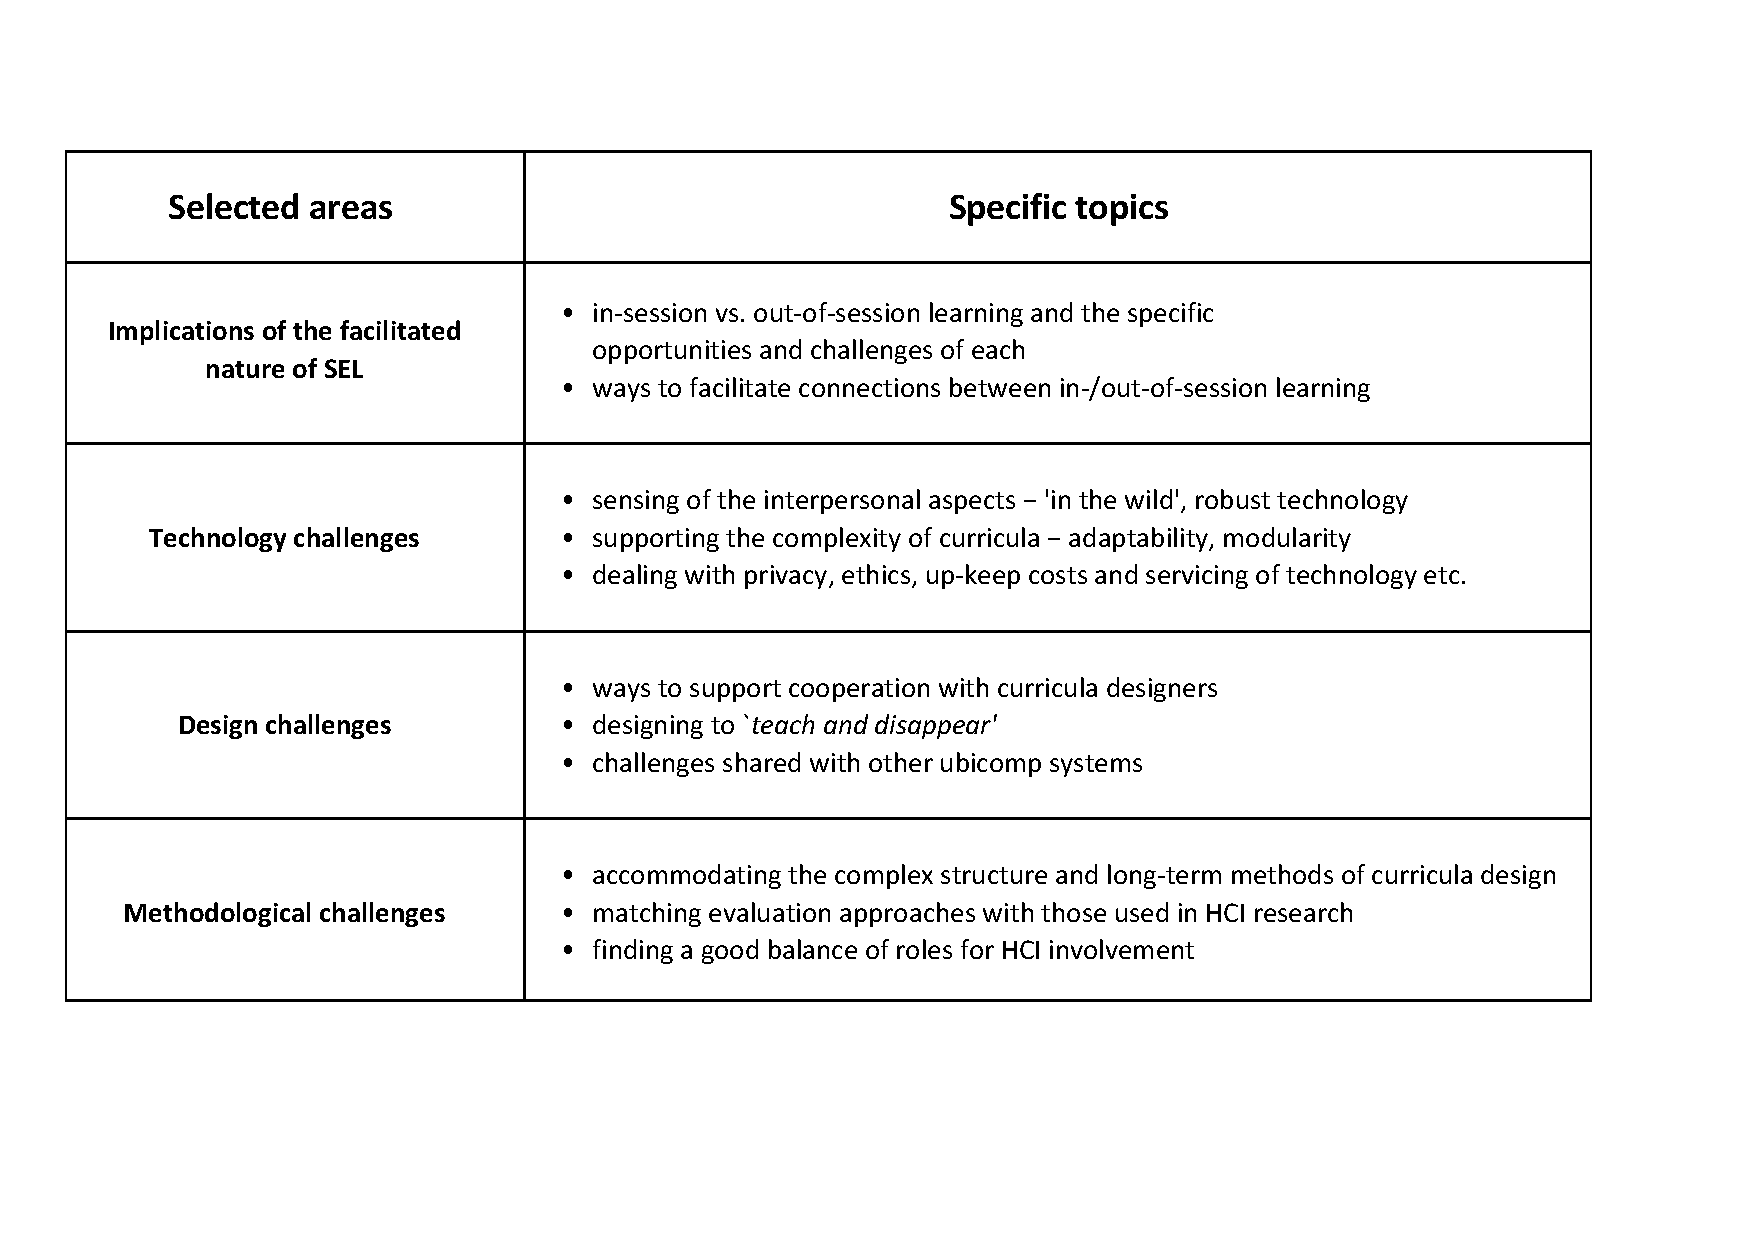
\includegraphics[width=\textwidth]{images/Section6Summary.pdf}
        \caption{Mapping out the design space of SEL -- summarising the areas bringing key challenges and opportunities for HCI research}
        \label{tab:session6summary}
\end{table}

\begin{itemize}
        \item We first discuss the {\bf implications of the facilitated nature} of the social skills learning curricula, leading to distinguishing inside and outside of the training session as two core settings for design of systems in this area. We outline how they differ in their affordances, possible target groups of users to design for, and the differences in what types technology could be most useful in each; also highlighting the need for technology that would help connect together the learning processes inside/outside. 
        \item Second, we discuss the {\bf challenges for technology} posed by the social skills learning space. We start with the two key technical challenges in this space: sensing interpersonal signals relevant to social skills teaching, and the need for adaptability and modularity of technology due to the complexity of the curricula to be supported. We then briefly discuss many other challenges that are shared with other ubiquitous applications (e.g., privacy, ethics, timely feedback, maintenance of deployed technology).  
        \item Third, we look at some of the {\bf design challenges} this space poses. Apart from the common issues again shared by other ubiquitous applications, we draw out two more specific aspects: On one hand, the focus on designing technology that facilitates or 'scaffolds' learning of skills, but is expected to be removed once the skills are learned. On the other, there is a potential for a large scale, real-world impact of technology that would get incorporated into curricula. However, this comes together with the design challenges connected to the complex, multi-disciplinary interventions to be supported, which involve many stakeholders and policy decisions as well as strict requirements on cost-effectivity and robustness of developed technology. 
        \item Fourth, we briefly outline some of the {\bf methodological challenges} brought by cooperation with large scale interventions and related research. These draw on differences in the structure and time span of research on educational curricula, and the approaches common in HCI. Similarly, the evaluation of the developed technologies might require novel methodology approaches, perhaps drawing on and re-appropriating the knowledge already existing educational and related domains. We conclude with a short discussion about what could be the role and contribution of HCI in this space.   
        
\end{itemize}

% {{{ Inside/outside implications
\subsection{Implications of facilitated learning -- possible settings}
\label{sec:facilitated}

One of the defining features of social skills learning curricula is the combination of facilitated teaching, i.e., learning under the guidance of an expert trainer, and the interplay between learning processes during and outside of the learning sessions. 
Table~\ref{fig:in-out-dim} flags up our brief discussion on how inside/outside of training sessions differ in terms of affordances, target user groups and types of technology that could be used. 

In particular, although one of the key HCI contributions to social emotional learning courses could be extending the learning support \emph{beyond} in-session learning, developing systems for the in-session contexts can be a good first step, both in terms of testing the technology, as well as being directly useful in supporting the facilitator's role and enhancing the learning experience. We suggest that in-session learning is an interesting design space in which novel technologies can be developed -- marrying the benefit of direct application into, and testing within, real-world scenarios, with the possibility to do so in a well constrained and manageable environment and with a facilitator who is an expert in both the content and the tools they use.   




\begin{table}
  \centering
        %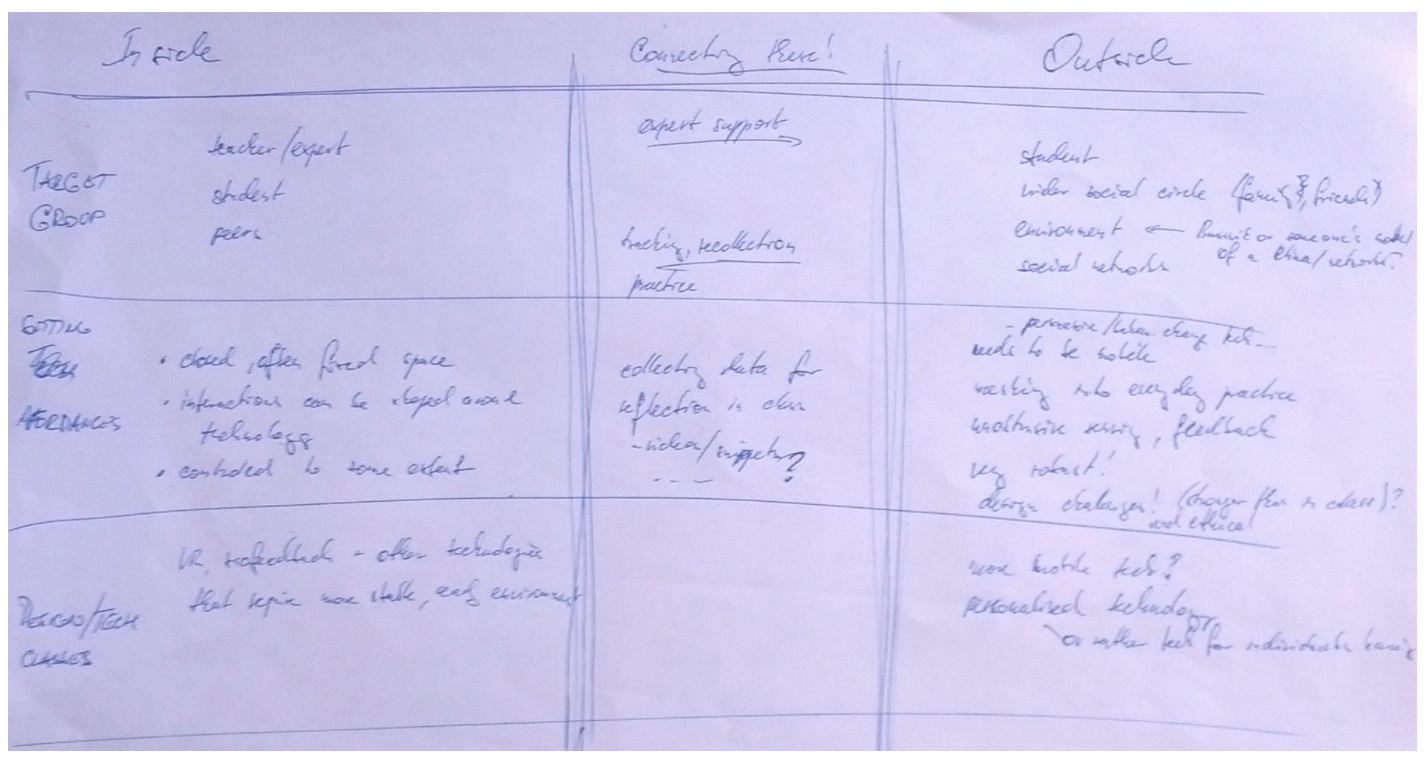
\includegraphics[width=0.8\textwidth]{images/In-out-sessionDimensions.png}
        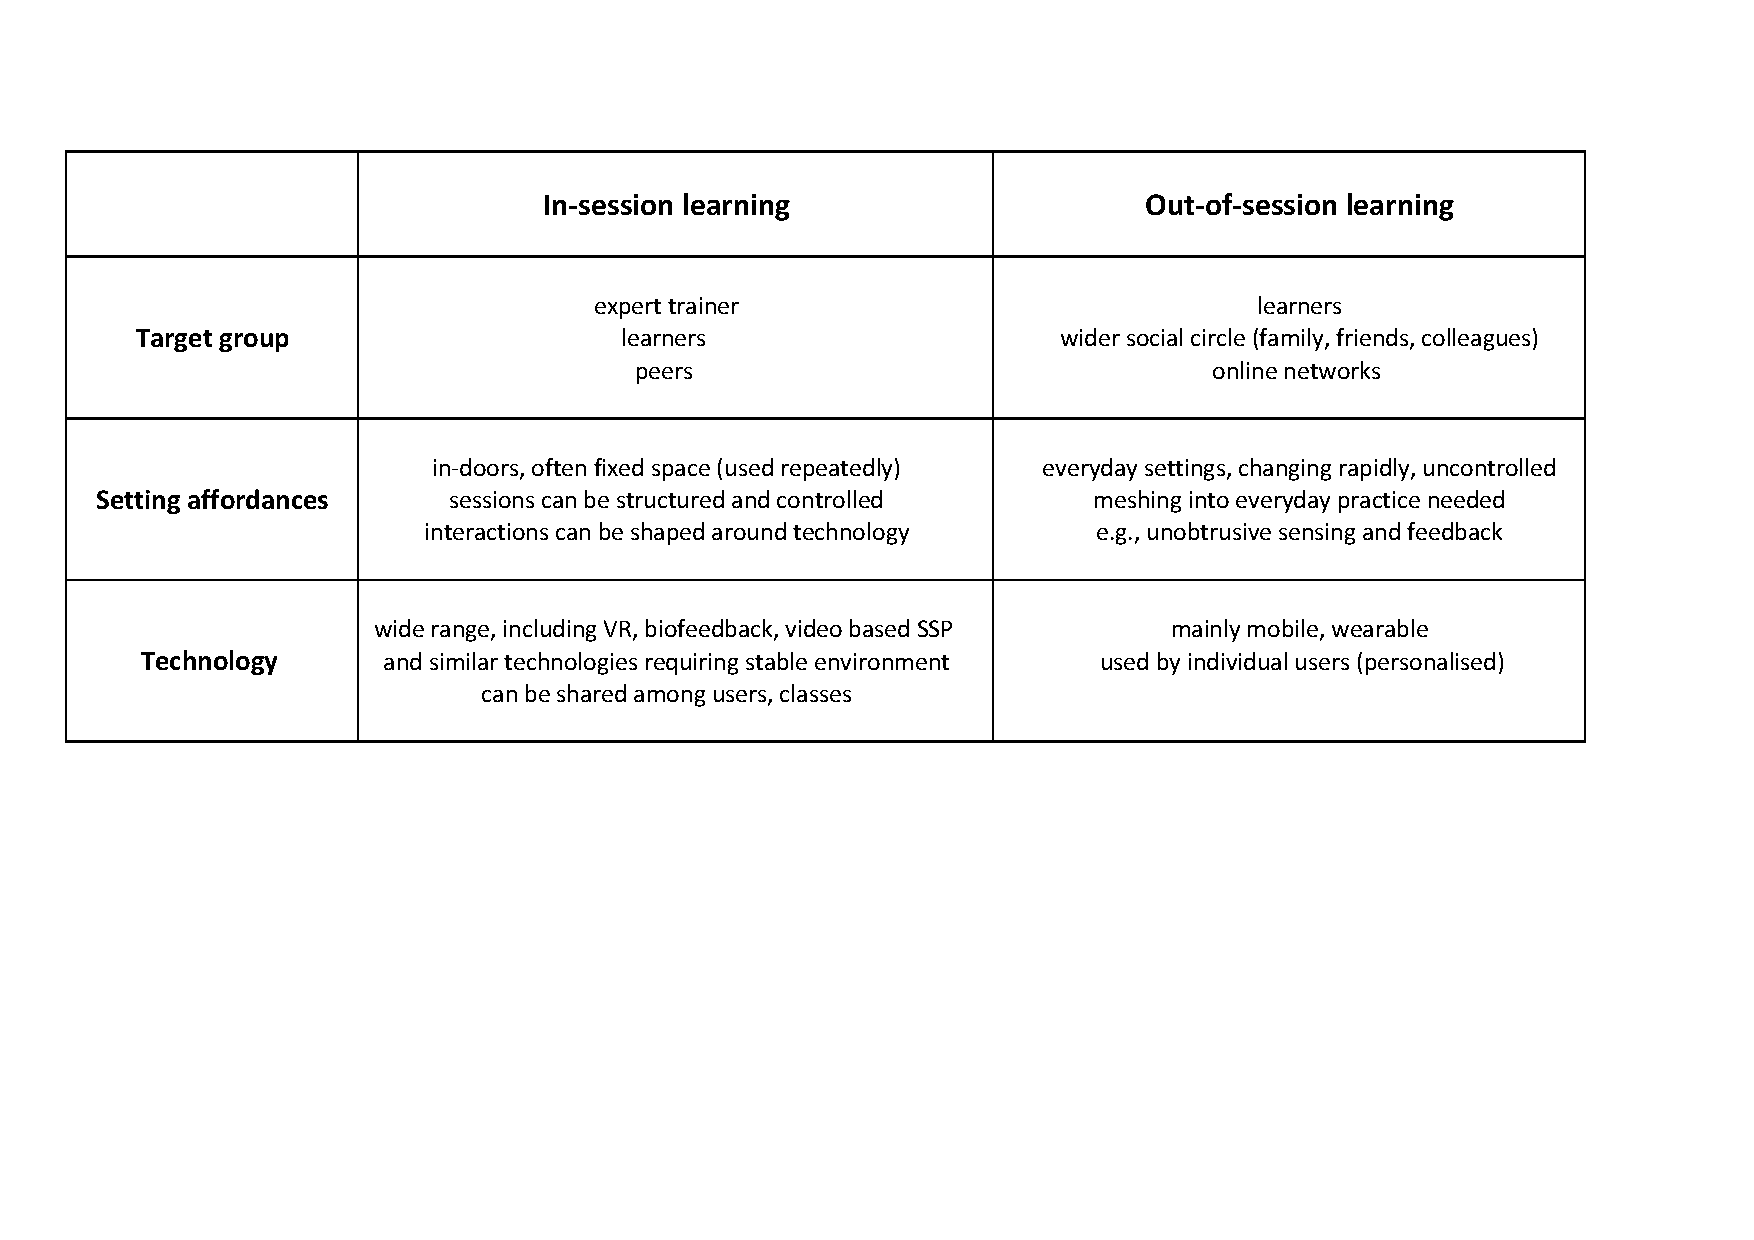
\includegraphics[width=\textwidth]{images/in-out.pdf}
        \caption{Summarising the key differences between in- and out-of-session learning settings}
        \label{fig:in-out-dim}
\end{table}


\subsubsection{In-session learning}
Learning sessions typically take place indoors, involving a mix of lectures and hands-on experiences, likely with an expert trainer/coach present. This leads to a limited, often quite controllable setting for technology deployment and points to particular user roles that can be designed for, such as supporting the trainer's expert role (augmenting and enhancing rather than replacing their skills), facilitating peer feedback or group reflection on examples, and directly supporting the individual learners.

Additionally,  the training experiences have a particular quality of being ``real'' and ``not-so-real'' at the same time: often asking participants to practise and try new skills out in a ``safe place'' (e.g., through role play), where potential failures in interaction are actually a valuable basis for reflection and learning, and the expert trainer can immediately assist if problems appear. In this sense, such in-session training is a `real' situation in terms of the learning setting, but fictional and `unreal' for the participants, and also a situation that is specifically open to, and designed for, external feedback and reflection. 

The combination of the in-class space and the specificity of training experiences potentially allows for a more intricate\GeraldineFIX{G: not sure 'pervasive' is the right word here - what do you mean here?\ is it that it can be rolled out to lots of training contexts, or that it gets dedicated/focussed use or? } technology deployment than would be possible in every-day life. Many of the pragmatic and ethical challenges present outside of the classroom are relaxed, such as the possibility to affect, interrupt and shape the interactions; being less difficult to obtain consent with data collection; %, which straightforward for in-sessions learning, but less so ``in the wild''; 
or the fact that the situation is role-played and thus (most probably) less personally sensitive for participants. Moreover, the 'controlled' training spaces have many additional advantages such as the potential for easier initial technology deployment and lower robustness requirements; or the potential for easy collection of training data corpuses for automated approaches such as social signal processing \GeraldineFIX{G: SSP - don't think this has been set up as an abbreviation before this? assume it is social sig  process?}or affective computing --- while still working with the "real" learning process (i.e., not an instrumentally designed laboratory task). The curricula are often well structured, with prepared exercises and model situations known in advance, which can also provide a focus for design work and ease initial deployment of technology. 


\subsubsection{Out of session learning}
Everyday life automatically offers many opportunities to practise social skills. Such practice serves an important role in most curricula as it supports successful transfer of learnt behaviours into learners' lives. 
%
The key issue is however that---in contrast to the in-session learning---learners can receive only very little support from the trainer or peers in these settings; thus skills that are not developed completely are hard to practise successfully. Learners can slip back into their old habits (perhaps not even knowing they are doing so), might not even attempt to try the skills (as the situation is too important), or would need external facilitation to practise successfully.  

This points to a number of roles technology is likely to support when facilitating learning outside of the class session. As discussed earlier, systems can focus on individual learners and possible ways in which they can be supported in their practice (e.g., through feedback) and reflection on their behaviours. Alternatively, technology might attempt to seed a supporting environment for the learners through facilitating involvement of their social networks such as family, friends, colleagues into the learning process, supporting peer interaction and support outside of the in-session, or even providing links for the trainer's intervention or support outside of the learning session (and as captured data for feedback in class as will be discussed below). 

The ``in-the-wild'', everyday setting has also implications for technologies used. The mobile and wearable nature of much available technology is likely to be key, together with the need to blend with and into everyday behaviours %(or practice in sociological sense -- \todo{ ask eva for a different word}) 
and still provide meaningful feedback or benefit. Given the interpersonal nature of many social skills, any sensing which might involve people other than the learner outside of in-session learning will need to address many additional complex design and ethical challenges. 

Still, supporting and facilitating learning outside of direct learning sessions is the key challenge for social and emotional skills curricula at the moment. We have also seen examples of HCI research in previous sections that have dealt with these successfully (e.g., \cite{Escobedo2012,Tentori2010,Matthews2011}), suggesting that it is possible to provide beneficial intervention even in such complex settings. 


\subsubsection{Connecting in-/out-session learning}
Another important area for technology support is supporting connections \textit{between}  in- and out-session learning. We envision that much has to be possible to extend the current ``homework'' approach used in the curricula, where the learners are asked to do particular exercises in between sessions and then report back (e.g., in person, and/or via an essay, diary record etc.)\GeraldineTODO{G: do these also need to be mentioned as explicit strategies in the discussions of the  learning principles and current approaches?   }.  Obvious examples of potential for technology support are to: track progress or practice; collect (video/audio) data to support post-hoc reflection or analysis within sessions; and support communication channels to get information/help from the peers or experts even when outside of the session (as discussed above). However, we expect many other, more sophisticated ideas are possible, each drawing on the particularities of the curricula and domain to be supported. An example of such technology, albeit aimed at learning mathematics rather than social skills, is from the Homework project \cite{Luckin2008}, where 5-7 year olds were given tablets and specialised software connecting class work, homework exercises, and facilitating parents' involvement and communication between parents and teachers.


%\subsubsection{\todo{Summary text:}} if needed. 
        
%       Majority of activities and learning aspect in all courses consist of \emph{facilitated learning}, regardless of the domain. We argue below that this points to an interesting design space in which novel technologies can be developed, marrying the value of direct application into and testing within real-world scenarios, with the possibility to do so within well constrained and manageble environment.  Whereas one of the key HCI contributions to social emotional learning courses could be extending the learning support \emph{beyond} classrooms and directly facilitated learning, developing systems for the such facilitated contexts can be a good first step, both in terms of testing the technology, as well as being directly useful to the teaching process. 
% }}}


% {{{ Technology aspects
\subsection{Technology challenges}
\label{sec:techAspect}
 There are also challenges that technology deployment will face in the area of social and emotional learning. While many of these are shared with other ubiquitous applications, some are more specific to SEL. First is the sensing and processing of aspects relevant to feedback on social skills that are mostly based on interpersonal interaction and complex concepts. Second is related to the complexity of many curricula and the need to make technology support particularly adaptable, modular and re-usable. 

\iffalse
% {{{
\subsubsection{Possible roles for technology}   We've seen a range of successfully deployed---or potentially deployable---systems in the previous section. However, the presentation there was structured according to the learning principles the technology could support, rather than the similarities in the role it plays. We illustrate below the roles we've seen so far, 
%We now discus according to the similarities in the role technology plays there rather than the learning principles they support:   %\rephrase{A rough distinction of the benefits offered by technology that appeared repeatedly could be to distinguish:}
        \begin{enumerate}
                \item {\bf Expert sensing:} Some of the systems rely on sensing and interpretation of behaviour, helping users draw out patterns they were not aware of before. Information can be presented in real-time, such as giving feedback on communication behaviour in meetings \cite{Kim2008,DiMicco2007}, or over longer periods of time such as in AffectAura \cite{McDuff2012}. Such systems often draw on and connect many disparate data sources. 
                
                %\todo{this is future?} taking over some of the feedback from the trainers/peers or giving additional one (\cite{fjklds,fds,fsd,fsd,sdf}). 


                \item {\bf Structuring activities:} Other systems aim to provide timely reminders to support users behaviour. They may provide data for the user to reflect and act on, but rely much less on automatic sensing and interpretative capabilities of technology, leaving the  interpretation to the user. Examples can be autism, e.g., \cite{Escobedo2012}, listing the appropriate actions the person should take and asking them to rate their performance (i.e., no sensing on the part of the system); personal reflection tools, such as Affect Diary \cite{Stahl2008} or [SenseCam ref]; or facilitating keeping of diaries in psychotherapy \cite{Matthews2011}.  

                \item {\bf Novel experiences:} A third role we saw systems take was facilitate or create novel experiences. This can be either by providing a 'new world' to behave in,  as per (serious) games \cite{Hailpern2011} and virtual reality \cite{Bouchard2012,Romano2005};  or by helping the users to get a novel perception of a particular behaviour such as through gamification of real-world experience or the magnified feedback offered by \citeN{Fox2009,Bailenson2008}. 

                \item {\bf Connecting and sharing:} Fourth role was in supporting connecting and sharing among larger groups of users. For example, facilitating cooperation of a larger number of users from the same course (Massive online courses?, plus ref from section 5.3), or reaching out to potential social support nets (family/social circle in Three Good Things). 
        \end{enumerate}

%\todo{The first two maybe don't work -- mixing together 'patterns over time' and 'making invisible visible', no clear distinction otherwise -- apart from the expert/non-expert approach. Do we combine these together then?}
        
 \rephrase{While this structuring is one of many possible, we believe it can be useful to illustrate the variety of options technology can bring. It also points to the complexity of the design space and emphasising that supporting a particular learning principle does not necessarily prescribe a particular role technology needs to take.} 
\todo{How to link to the challenges section below? What is below not is pathetic:)}

We now discuss the technical challenges faced by most future systems in this domain. 

%These apparently go across the learning principles ... \todo{but what of it? Any table?} can be combined etc. ... How did they address the challenges? Difficulties? 

%\todo{This needs a lot of work!}
% }}}
\fi

%\subsubsection{Specific challenges for technology}

%\rephrase{A bit of leading text should be here -- plus I'm still thinking about how to make the visual structuring work here (as I want to put the two specific aspects under one section, but make them obviously visible)}


\subsubsection{Sensing of interpersonal aspects} Automatic capture and processing of data that is robust and reliable is often difficult in the wild, especially if it is to be meshed fluidly with other complex interactions (as will be the case in both in-session and out of session systems here). However, sensing and processing of aspects relevant to social skills is likely to be challenging by itself, even in controlled laboratory conditions.

This is partly due to the interpersonal nature of the sensed data, which has not been common in social signals processing, affective computing or related fields that focus so far mostly on individuals \cite{Vinciarelli2012}. Additionally, many of the social concepts taught in the courses are holistic and are yet to be defined in a way that would allow automatic sensing; it might even be impossible for some. Support for social and emotional skills courses thus raises many well-motivated research questions around which aspects can be sensed and interpreted\footnote{An intriguing parallel can be seen in psychology of interpersonal judgments, where a large body of research shows that human raters can reliably judge complex concepts such as perceived warmth or friendliness of a conversation on the macro level (gut instinct), but even after many studies micro-coding many of the non-verbal signals (head nods, movements etc.), it is still unclear what cues raters draw upon to make their intuitive judgements \cite{Ambady2000} or \cite[p.299]{harrigan2008}.}, and whether that is possible on the individual or interpersonal level (i.e., combining sensed data across participants).

There is also a question of the level of interpretation we expect the system to provide. This leads to a continuum from leaving the sense-making of raw data entirely to the user and/or the facilitator (e.g., as per SenseCam systems \cite{Fleck2009}), to providing full interpretation by the system (e.g., as in arousal detection for people with autism \cite{Picard2009}). Even if particular concepts cannot be reliably and fully interpreted by technology, it might still be possible, and in many cases actually preferable, to support the users by providing a 'reasonably' pre-processed data they can view, interpret and reflect on.



\subsubsection{Complexity of curricula -- need for adaptability and modularity}
Another challenge is posed by the complexity of curricula, the wide range of skills that are usually taught and the developmental/progressive nature of skill acquisition. This suggests the need for modularity of the designed systems and preference for highly versatile and re-usable designs that can be adapted for teaching many aspects within the curricula and personalised to individual learning paths. %\rephrase{Immediate ideas are either to support an underlying process (e.g., reflection) in such a way that it can be applied to multiple scenarios, or }
%
%
Cost-benefit ratio and robustness of the system will be also important, both in terms of durability and reliable sensing in difficult real-world environments, regardless of context and setting. These will be especially crucial if the aim is to deploy technology as a part of existing curricula. 
%
Technology will also need to adapt to the differences among domains and settings, and the related variances in the length, focus and breadth of curricula, even when supporting a concept important across the domains (such as self-reflection). For example, we expect differences between designing for young learners (such as in education curricula and psychotherapy for adolescents) and for adult learners (e.g., in business and medical domain courses); and differences in supporting social skill acquisition for professional versus personal motivations.

\GeraldineTODO{G: could reference here something from the PAL\ project   and their AIRS platform and/or the MyRoR platform as technical architectures specifically aiming to support such adaptive modularity    }

%  -- e.g., point to the differences in social judgements on macro and micro level 
\subsubsection{Challenges shared with other ubiquitous systems} Many of the challenges in this design space are shared with other ubiquitous computing applications. For example  providing timely, unobtrusive feedback is often a challenge for ubiquitous applications, even if the sensing and processing issues described above are resolved; as are issues around managing and keeping the technology running once deployed. Privacy needs to be addressed whenever a system includes sensing or data collection,  especially so if the goal is to sense interpersonal aspects of an interaction. Finally, ethical concerns regularly arise, particularly when working in sensitive settings such as education of young learners or in the medical domain. 
For a more detailed discussion of such issues in other contexts see e.g., \citeN{Caceres2012}, \citeN{Consolvo2007} and \citeN{Kientz2007}.
% }}}


% {{{ Design challenges
\subsection{Design challenges}

There are also many design challenges shared with other ubiquitous systems, but some are quite specific to SEL. We discuss two such key aspects. First is a combination of an opportunity and a challenge: the potential for large scale, real-world impacts \emph{if} the technology is accepted by the curricula design community. This however brings the need to closely cooperate with curricula designers and address serious challenges due to the particularities of the setting, the interdisciplinarity of such projects, the interactions with policy makers etc. Second is designing technology as a temporary scaffold not as a permanent crutch, i.e., designing with the aim to help teach new skills over a limited period of time, after which the technology is expected to be taken away or no longer needed, and where the skills persist. 
Finally, we then highlight the more common ubiquitous technology design decisions, drawing out those that might be particularly relevant to the SEL area.
 
%\subsubsection{Specific challenges} \rephrase{Same issue with the leading text as per above ... }
%\label{sec:designSpecChal}
        \subsubsection{Need for cooperation and knowledge sharing with curricula designers}
        The learning principles identified earlier---together with curricula descriptions available in literature---are likely to help initial explorations of the design space. However, developing systems either in collaboration with curricula designers, or directly for specific existing curricula will be crucial for real-world usefulness and deployment of the developed systems. %In other words, it doesn't make sense to design and deploy new curricula within HCI, but rather cooperate with curricula designers and use their knowledge to jointly find most effective and beneficial ways to include technology into novel or existing curricula designs. 
        \citeN{Coyle2007} have discussed this issue with respect to designing for the mental-health domain;  \citeN{Porayska-Pomsta2011} address the challenges of similar interdisciplinarity in designing for autism. We will argue in the next section how their approach can be extended to the whole setting of social and emotional skills, and return to the methodological challenges brought about by such interdisciplinary cooperation. 

%Their arguments based on lack of access of HCI researchers to mental-health treatment settings due to many aspects, e.g., ethics. While some aspect of education or bussiness areas raise lower ethical issues than mental health therapies, it will still be crucial to draw on the long-term knowledge of curricula design professionals and cooperate. 

\subsubsection{Designing to ``teach and disappear''} Most social and emotional skills courses, irrespective of domain, run only for a limited time. This can often be as short as a few hours or a weekend; or span longer time periods, but possibly limited to several hours every week (e.g., as in K9 school curricula). 
In both cases, the aim is to facilitate development of new skills over the duration of the course, and it is crucial that the skills become embedded enough to persist even after the course is finished. 
Although it might be relevant for some cases to develop technology that allows to extend or supplement the course duration, the ultimate goal of technology is likely to scaffold and help learn skills that will stay available \emph{after} the technology is taken away. This provides interesting and novel challenges to designing systems, especially with the potential to enriching approaches used in behavioural change and related fields. Additionally, such a focus calls for designs that can adapt and follow the learning curve of students, always supporting the next `zone of proximal development' \cite{vygotsky1987collected}. 


\subsubsection{Design challenges shared with other ubiquitous systems}
        Designing for social and emotional skills is also likely to raise many issues that have been already widely discussed in earlier work around ubiquitous systems and related technology. These can be challenges around privacy and the degree of control given to users; need for adaptability and personalisability, as well as designing with sensitivity to different cultures. Other factors will likely involve decisions around making the technology individualised or shared by many; the feedback style (give ``expert'' opinions, or leave interpretation open to users) or feedback mode (ambient vs. explicit feedback), as well as the need to include many potentially competing requirements (e.g., the need to address most if not all learning principles). Pragmatics will also come into play including issues around designing for difficult settings (e.g., schools with high violence and poverty rates); or supporting training and ease of use of technology for trainers and learners, especially in large-scale deployments.  %As described earlier, the designs will also need to address most if not all learning principles in each system.
See, e.g., \citeN{Consolvo2007} or \citeN{Rogers2007} for an in depth discussion of similar issues.
% }}}

% {{{ Methodology 
\subsection{Methodological challenges}
Research on social and emotional skills will likely also bring  novel methodological challenges, especially if the aim is inclusion or co-design of the technology in large-scale curricula projects, and its acceptance by curricula designers and policy makers. Here we focus mainly on such co-operative projects, as these are likely to have the highest potential for large-scale impact of HCI research; but also present specific challenges. We discuss three interrelated issues: structure and methods usually imposed on research in curricula design projects; the approaches to evaluation in these domains; and the possible roles HCI could take in this space. 

\subsubsection{Structure and methods}
Curricula tend to be very complex, large scale interventions, especially so in the education and the medical settings. Designing technology for these settings will need to take into account the longer term time-span and intense focus of research projects in these domains, where it is usual to take many years to develop and test a curriculum. For example, \citeN{Matthews2011} show how such co-operation is possible and discuss the development, deployment and clinical trial of a mobile-phone support for psychotherapy with adolescents. 

Although it is potentially challenging to accommodate this in the quicker turn-around of projects usual in the HCI space, such sustained focus and long-term research agendas may have a beneficial impact on research on social skills and interaction within HCI more generally. Whereas existing HCI work on teaching social and emotional skills has been mostly fragmented (except perhaps for autism research), often in the form of single studies, with little long-term follow-up, the structure inherent in SEL curricula might promote more systematic research and lead to highly successful, real-world applications. Such projects could enrich HCI approaches with methodologies, contexts and goals that are well defined, well researched and very well motivated by real-world needs. 


\subsubsection{Evaluation approaches}
Approaches to evaluation methodologies also tend to differ between curricula designers and most of HCI work. There is a push for an ``evidence based'' support for curricula interventions, as required by the policy makers. This leads to a sequence of increasingly complex studies, starting from formative, small pilot studies that test viability of particular ideas; through larger, longer term studies to confirm potential; and eventually building up to multi-site trials, often in the form of randomised control trials or similarly resource intensive methodologies such as complex quasi-experimental designs, which are less common in HCI.  So although there is a mix of qualitative and quantitative methods inherent in the design and initial exploration of curricula, there is a call for mostly quantitative methods to test the effects of a developed curriculum on outcomes in the long term. There is also the potential for HCI\ to influence these evaluations with a complementary focus on the processes and interactions through which such outcomes are achieved. This can impact the roles HCI might take in this domain, as discussed in the next section. 

%Additionally, it will be challenging to develop, or find already established, methodologies to support the initial short term, iterative design of systems important for HCI.


\subsubsection{Roles for HCI}
The complexity, scale and dependencies of such large-scale projects necessarily affect ways in which we as HCI practitioners can engage.  An extensive discussion of similar issues in related domains is already available. 
%, as already discussed in section \ref{sec:designSpecChal}. 
%
For example, \citeN{Coyle2007} suggests a two stage process in the area of talk-based therapies, where the first exploratory part is led by HCI with cooperation from experts from the other domain, aiming to iteratively develop and run initial evaluations of promising systems to the point ``where they are shown to be usable by the target end users, are agreed to have clinical validity and are predicted to have therapeutic benefits.'' Stage two then focuses on larger scale evaluations and the roles exchange: the lead is assumed by the curricula experts with HCI researchers in a collaborating role, and receiving feedback on the systems use in real-world practice.
\citeN{Fitzpatrick2012} discuss similar issues in their review of CSCW systems in medical settings, arguing for the need to engage with and raise awareness of CSCW (and HCI related) issues with many of the stakeholders. 

We suggest a combination of the \citeN{Coyle2007} model of cooperation with curricula designers, complemented %for social skills learning systems, aiming to develop systems with immediate practical use and deployment; 
with another stream of more independent, smaller, exploratory studies that try to push the boundaries of what might be possible to do with technology in the first place.  In other words, we can see benefit in parallel research on two areas: (i) aiming for large scale, real-world impact with technologies/ideas that are already matured in HCI, in close cooperation with curricula designers and large interdisciplinary projects; and (ii) more exploratory HCI process, that draws on existing curricula and the challenges, bringing novel, untested technology and exploring a broad range of viable approaches that eventually feed into the first stream. It is our hope that this article could inspire future work pursuing either of the two direction. 


%\todo{WHOLE SECTION NEEDS MORE MEAT -- feels it has been only skimmed and most discussions deferred to other papers}  
% }}}

% {{{ Old text -- iffalsed

\iffalse
The previous sections unpacked the learning  principles identified earlier, linking them to existing work within HCI and pointing out how such \rephrase{combination} might be especially useful for SEL, by providing novel opportunities to teach and learn social skills.  
This section highlights the challenges and opportunities doing so might raise for HCI. 

% %Previous section discussed ways in which HCI could help support teaching of social and emotional skills as well as address challenges existing within SEL learning curricula.  as well as for HCI through \rephrase{interacting} with an interesting new domain for which useful applications can be developed and, by doing so, inspire further research within HCI.



Focus on social and emotional provides a way of structuring and inspiring novel research on social interaction within HCI by bringing methodologies, contexts and goals that are well defined, well researched and very well motivated. Whereas existing HCI work on teaching social and emotional skills has been mostly fragmented, often in form of single studies, with little follow-up or elaboration, the structure inherent in SEL curricula might promote more systematic research, higher comparability of and building on existing studies, and lead to highly successful, real-world applications. 
%
For example, the goals of social and emotional skills learning are complementary with existing HCI research that focuses supporting, enhancement and automatic analysis of social interaction, suggesting novel and well-motivated real-world applications for much of social signal processing and related research. 
%
Moreover, the topic of SEL within education also gains increasing political support in the US and Europe \todo{refs -- e.g., Seligman2009,Cohen2006}, suggesting that social and emotional learning programs for schools might be soon included in most schools. The situation is similar also for the other domains, with SEL programs already flourishing in business and being on the rise within the medical domain. Overall, SEL provides a novel design space for HCI that could have a strong, positive impact on everyday life of a large population. 

More generally, training contexts such as the courses described here are an interesting design space in and of themselves as they could provide a valuable initial context in which to consider the design of other novel systems supporting life skills teaching and long-term development. Such training contexts keep all the \rephrase{positives} described in the Facilitated learning section \ref{sec:facilitated}. It also leaves open opportunities for technologies (and practice situations) that could not be applied in everyday settings for various reasons, such as simulating situations and interactions that are potentially dangerous or emotionally challenging.



        %\item Of interest for HCI is also that most of the curricula take training of the teachers very seriously, suggesting another potential settings where novel technology could be utilised and be very useful.


% {{{ Challenges for HCI
\subsection{Challenges for HCI }
        \begin{itemize}
                \item \todo{key questions we need could look at: } e.g., what are the limits and potential of current social signal processing in terms of tracking such skils? Are they applicable in real-world use? etc. 

                Behavioural change application outside of energy consumption, well-being? 
                \item while there is a broad potential for application within the existing curricula and courses, doing so will require robust technology and cost-efficiency aspects, especially if one aims for a wider deployment.
\item Efficient communication: Related to the issue of cost efficient wider deployment mentioned above, a potential system for SEL needs to support efficient communication between a coach/trainer and a large number of students. This entails providing a high level overview of the student cohorts progress and providing pointers to individuals and situations where feedback from the trainer is indicated without overwhelming them with every detail that the system is currently tracking. This entails the need for the development of machine learning (big data) approaches that help to differentiate between situations which could be successfully handled by the system and where an intervention by the trainer is required.   
                \item How do we deal with the need for interdisciplinarity, as identified by \citeN{Porayska-Pomsta2011} or \citeN{Coyle2007}. \rephrase{Emphasise the need for co-development with the practitioners. }
                \item Real systems will need to combine most of the challenge categories above -- example of MOSOCO, which helps receive peer feedback, aims to support practice in the wild, and keep engagement through gamifying the situations (earning stars, comparison etc.). 
%               \item Successful examples of autism related systems ==> how will similar approaches extend to NT conditions, where most of the processes taught are much less structured, harder to track, and even specify?
\item balancing necessary user tracking with privacy concerns:  As SEL involves vulnerable user groups such as students and confidental situations, e.g. doctor-patient communication or psychotherapy settings, the technologies used to facilitate practice and to foster the embedding of these skills into everyday situation need to guarentee the privacy of the involved parties. This is particularly important during facilitated learning, where feedback from a trainer is a crucial component. The system needs to enable feedback by the trainer/coach by giving them the necessary information about the learning situation but do so without revealing any details about the involved stakeholders without their consent. 

        \end{itemize}
% }}}

        %Moreover, funding schemes supporting use of SEL curricula in schools exist in the US [\rephrase{can use the links from earlier version, e.g., US National Research Council}]. In addition, several governmental or non-governmental agencies compiled reviews and ratings of available curricula, to ease decision making process for schools. These include \todo{CASEL, Blueprints for Violence, the UK reviews, and others}. 

\fi
% }}}

% }}}
\fi 




\iffalse
% {{{ SECTION: Summary of life skills 
\section{Summarising SEL -- four learning principles and associated challenges}
\label{sec:summary} 

The previous section outlines the general agreement on core skills and general approaches to teaching these; albeit interpreted specific to contexts (theories) and age ranges of pupils/teachers. In particular, all these teaching methods and approaches draw on a common dependence on procedural learning -- see Table~\ref{fig:SummaryResults} on page \pageref{fig:SummaryResults} for an overview. 

\subsection{Four learning principles}
Based on these similarities, we draw out a set of four 'learning principles', with each principle pointing to particular challenges to social and emotional skills learning. We frame these principles with HCI research in mind, distinguishing them here in order to highlight particular issues that HCI designers and researchers could consider supporting, \rephrase{as part of adressing the specific topics (such as self-awareness etc).} 


In this sense, they provide a set of perpendicular aspects, common for all the skills described earlier. By pointing to particular approaches and methods, it is our hope they help to outline more clearly how social and emotional learning could tie in with, and benefit from, HCI interests, guiding future work on this topic. 

We emphasise however that they should not be understood as independent, reified concepts. They are obviously interrelated and dependent on each other, and it is likely that any real-world system will draw on multiple if not all of these aspects, although perhaps focusing on some more than the others as relevant.


We list the four principles below, and then discuss each in turn: 
\begin{enumerate}
        \item providing cues for reflection;
        \item facilitating practice;
        \item embedding and transferring skills into everyday situations;
        \item supporting motivation and engagement of the learners.
\end{enumerate}


%Figure~\ref{fig:sum-challenges} places all four principles into context: Feedback and practice play a central role in learning social and emotional skills, regardless whether within or outside of the learning contexts. Supporting transfer of learned skills by embedding parts of learning into everyday contexts and real-world situations is then one of the key goals in the training reviewed above. Additionally, learning experiences need to be engaging and motivating to be successful. 

\paragraph{Supporting the reflective abilities} \todo{Base on the experiential learning as a main concept}
As social and emotional skills are very complex and challenging for learners to track easily by themselves without external support, all curricula facilitate various ways to give the learners feedback on their behaviour. However, providing timely feedback is difficult.  Within the facilitated training sessions, the expert trainer or peers serve as the key source of feedback. A challenge though is that this  feedback mainly happens in a post-hoc manner, and often from unguided recollection of what  happened during the practice. Moreover, the ratio of trainer to students  commonly means that learners get feedback mostly from their peers, who are not trained or particularly skilled in what is taught.
Outside of the facilitated sessions, any form of feedback is virtually impossible, and often ends up relying on the student's self report of  their own attempts  
to practise when they come back to the facilitated session.
\begin{itemize}
	\item \qq{Cohen2001}{Promoting reflective capacities, that is, an ability to read ourselves and others, is the first core concept of effective SEL programs. It is the foundation for all learning.}
	\item \qq{Moon}{Experiential learning... copy and paste some stuff from there?}
	\item \qq{Pasi, p12}{Students need opportunities to problem-solve with others and to examine what worked and did not work in those interactions and collaborations. To develop their self-knowledge and capacity to deal effectively with others, students need a range of opportunities to apply decision-making and problem-solving skills to various situations. The educational goal becomes more than the end product, final presentation, or project; it includes an examination of how the student (and her peers) worked together. What behaviors and attitudes helped the group; which hindered? What are the characteristics of effective and ineffective collaborators in group situations? What are the strengths each person brings to a cooperative learning project? Through varied experiences, students can develop the skills and habits that will help them beyond school and throughout life.}

	\item \qq{Elias, p25}{Many of these skills are basic to human functioning, so they begin to appear in rudimentary form in infancy. As children get older, they apply these skills to increasingly complex situations and learn to differentiate, label, and integrate them. Even in adolescence, skill development continues, primarily through the feedback, reflection, learning, and growth that result from new experiences. Helping students develop and coordinate skills in emotion, cognition, and behavior is a necessary activity at the classroom, school, and, ideally, district levels (Shriver and Weissberg 1996, Weissberg and Greenberg 1997)}
	\item \qq{Zins, p.177}{Fourth, building protective factors (e.g., promoting reflective thinking, problem solving, and the ability to accurately anticipate and evaluate situations) that decrease maladjustment is important. Promoting these protective factors also contributes to the amelioration of significant underachievement and promotes skills and the prevention of ado- lescent problem behaviors (e.g., aggression, substance abuse, dangerous risk taking).}
	\item \qq{Zins, p.81}{The second approach is to emphasize skills that are likely to generalize across settings and situations. Self-management skills, for example, involving planning and deliberation, self-monitoring and self-reflection, are applicable to practically all domains of life. Some learning skills, including strategies for acquiring knowledge and learning from feedback, also are likely to generalize.}

\end{itemize}

\paragraph{Practice} Opportunities for practice are absolutely key for procedural learning. Support for personal experience and hands-on exploration of the skills is thus present across all of the reviewed domains and training approaches. Within the lessons, practice opportunities range from simple model examples that are role-played to trying to utilise situations that occur naturally within the classroom for opportunistic practice. It is however hard for current curricula to go beyond a short-term role-play. This is especially so for topics that are ethically challenging such as responding to conflicts or emotionally loaded situations. And it is even more challenging to design ways to support learners in extending the (controlled) practice opportunities beyond of the immediate teaching interaction.
\begin{itemize}
	\item \qq{Pasi, p12}{}
	\item \qq{Elias, p.55}{Guideline 8 - Whether applied to recognition, scientific notation, irregular verb conjugation, or SEL, repeated rehearsal using many different instructional modalities provides benefits (Ladd and Mize 1983, Mize and Ladd 1990). There is one main difference between SEL and many academic subjects, however. While SEL entails the learning of many new skills, it may also require the unlearning of habitual patterns of thought and behavior. For instance, students rarely come to class having repeatedly practiced an incorrect version of the multiplication table, but they may have become well schooled in not waiting their turn or not listening carefully to others.}
	\item can get many others I assume 
\end{itemize}

         
\paragraph{Embedding and transfer of skills} The ultimate goal of all social and emotional skills training programs is to transfer and embed the skills learned in the classroom context into everyday behaviour and real-world situations. By embedding we mean transforming a skill from one that can be enacted when prompted (e.g., in a practice session) into a skill which becomes an automated, nearly habitual response  in everyday settings and situations.  
        %

\item \qq{Elias, p.56}{When individuals feel anxious, angry, or sad, their ability to solve problems or concentrate on learning diminishes (Forgas 1994). Students who have shown improvements in their behavior may revert to earlier, more dominant habits when emotions are strong. When this happens, it is as if the “thinking brain” in the frontal cortex is overrun by the more automatic responses of the subcortical limbic system (Damasio 1994, Goleman 1995, Sylwester 1995). To avert this occurrence, social and emotional skills must be strengthened through practice in a wide range of contexts. Direct facilitation of classroom instruction may be provided by teachers, school counselors, psychologists, social workers, or paraprofessionals trained in SEL. ...  all personnel play an important role in actively encouraging and reinforcing the use of skills and attitudes they see displayed. Throughout the day—on the playground, in the halls, in the lunchroom, on field trips, on the bus, in aftercare programs—every adult has the opportunity to help students in reallife situations use what they have learned in the classroom. Typically, this practice is aided by reminders, usually in the form of tangible prompts. }

        Curricula currently approach this, on the one hand, by including real-world examples and situations within the learning context (e.g., asking students to recall and discuss particular experience they had, or having doctors and therapists analyse data from their own practice) and, on the other hand, by attempting to extend the learning context outside of the lessons or therapeutic session. Examples of attempts to extend training beyond the class include: trying to increasing awareness (e.g., posters placed around the building); scheduling follow-up meetings to support recollection of what was learned; and asking the learners' social networks to help reinforce the learning and skills in between sessions.
        % 
        However, the current approaches are limited in scope and effectiveness, and there is little that curricula designers can do to directly influence embedding outside of the learning sessions. As such, this learning principle poses challenges that could perhaps most benefit from technology support. 

\paragraph{Motivation and engagement} Supporting motivation and engagement of the learners also plays a major role in all learning experiences and is acknowledged as a key aspect within SEL for education, and increasingly also across all other domains and curricula. Existing work in HCI around creating engaging experiences suggests a potential to augment many aspects of the curricula, making them more engaging and thus motivating for the learners.
\GeraldineTODO{G: breaks the pattern as previous aspects haven't really mentioned HCI work in this way - lose here and replace with how motivation is currently handled???} 
%Methods used strongly depend on the topic, target group of learners and outcomes the curricula aim to achieve. 

\iffalse
\begin{figure}
  \centering
        \includegraphics[width=\textwidth]{images/challenges}
        \caption{Diagram of the identified learning  principles and their relationships}
        \label{fig:sum-challenges}
\end{figure}
\fi


\smallskip

In addition to the four learning principles, we also highlight the importance of the \emph{facilitated nature} of most social and emotional learning, pointing to a strong distinction between the directly facilitated learning processes available within the class context and learning outside the class in real-world situations. We will argue later, in section~\ref{sec:facilitated}, how this facilitated learning context opens up particular opportunities for thinking about technology support for SEL -- it combines the benefits of a reasonably controlled setting (i.e., teaching curricula with mostly well defined structures; mostly inside a specific room; and facilitated by a SEL expert), but still allows for designing systems for use in real scenarios (i.e., the learning context). This could especially be interesting for initial deployment and exploration of the novel technologies in support of social and emotional learning. 
%\smallskip

\smallskip
In summary, the four principles point to the key challenges we identified in the existing SEL curricula, and provide a link between the curricula and the potential to support SEL by HCI research. Figure~\ref{fig:sum-challenges} then shows the relationships between the four principles, and puts them into context. Feedback and practice play a central role in learning social and emotional skills, regardless whether within or outside of the learning contexts. Supporting transfer of learned skills by embedding parts of learning into everyday contexts and real-world situations is then one of the key goals in the training reviewed above. Additionally, learning experiences need to be engaging and motivating to be successful. 





\iffalse 
% {{{ OLD - similarities 
\subsection*{Similarities in topics} Although the exact skills taught are specific to each domain, all share interest in supporting aspects of two broad categories of skills: 
\begin{enumerate}
        \item First are various aspects of {\bf emotional awareness}, including understanding and reflecting others' emotions as well as being aware and managing your own, dealing well with stress or controlling strong feelings. Examples can be the skills identified for SEL in education withing the first two topics, i.e., identifying emotions and self-control. Similarly, the core emotional intelligence exercises in business involve various facets emotional awareness, as do the personal reflection or stress management parts of medical courses. 
        \item Second category focusses on {\bf communication and relationship skills}, mostly building on emotional awareness. These can be the ability to emphasise, cooperate, take perspective and constructively deal with conflicting situations and hard decisions. In particular, the third and fourth topic identified for SEL are directly relevant, as is the emphasis on conflict management, leadership and interviewing in business settings, and patient interviewing or empathy training  in the medical domain. 
\end{enumerate} 

However, these categories are very broad and each domain is aiming to support slightly different aspects. It thus important to go deeper into the particular topics of the chosen domain to reach more detailed understanding of what aspects are emphasised, taught and how (similarly to what we attempted to outline for SEL in education). 

% to use them as the basis for drawing out a coherent research agenda of opportunities for technology support -- it would be necessary to 

%\vfill ~ \pagebreak
\subsection*{Challenges for curricula designers}
%%%%%% rubbish starts :) %%%%
Curricula designers face several key challenges across the domains. These concern methods for providing (preferably real-time) feedback on learnt skills, ways of supporting learning experiences beyond the immediate scope of the facilitated training sessions.  

Providing timely feedback is difficult even within the facilitated training experience, especially as it is the trainer or peers who serve as the key source of feedback. This leads to receiving feedback in a post-hoc manner, mostly from unguided recollection of what was happening during the practice. Moreover, the trainer/students ratio often implies that learners get feedback mostly from their peers, who are not trained or particularly skilled in what is taught.  

It is even more challenging to design ways to support learners in extending the learning experiences beyond of the immediate teaching interactions, which is however key for sucessful transfer of skills into the real world. 

It is particularly difficult to instrument and support the practice of pupils outside of the learning lessons without technology in other ways than voluntary homework, or provide support to help learners embed the learnt skills into their everyday practices. Providing any feedback on behaviour outside of the teaching session is also problematic for the current curricula, leaving restrospective discussions based on recall as one of the few available options. 

By helping to address these challenges, HCI involvement could fundamentally augment and enhance the possibilities of existing courses, plausibly leading to novel and more effective learning and teaching methods. 

%While the courses across all domains have been shown to be effective, there are still challenges common to many of them. 

%One of the key ones is supporting and extending the learning experiences \emph{outside of the classroom}.  

%Moreover, we also see a high potential of technology to further support and augment existing teaching approaches within the classroom. We envision opportunities for support also for the remaining three teaching process principles described above, such as providing additional feedback opportunities (e.g., in real-time), environments and situations for practice (e.g., virtual reality or game environments), as well as helping to make the learning more engaging. The next section describes this in detail together with how doing so might also raise interesting novel questions and issues for HCI. 
% }}}
\fi


 % }}}

%{{{ Challenges 
\subsection{Summarising SEL learning in education}
%As outlined in more detail in section~\ref{sec:HCIsupport}, this is one of the core aspects where HCI could contribute.

\begin{itemize}
	\item 
\end{itemize}

% {{{ Key approaches/techniques? 
\subsubsection{Drawing out key approaches/techniques?}
\todo{Molecular, molar and global concepts to be taught}. 

\todo{Add things around social information processing as key --Zins,p.83} 
\todo{Also \qq{Cohen2001}{“R”--reflective capacities or an enhanced awareness of ourselves and others--is the foundation for all learning and development;Reflective capacities involve personal and an interpersonal component that provide a person with the ability to understand and learn from social emotional experience}}



% ZINS SKILL SELECTION STRATEGIES
The curricula take some or all of the three approaches outlined below, following \cite[p.81]{Zins}: 
%
\qq{Zins}{The first is that specific intervention goals may entail an emphasis on particular skills. For example, many SEL programs consider the prevention of violent and antisocial behavior a top priority, and therefore emphasize conflict resolution and related skills. 
%
The second approach is to emphasize skills that are likely to generalize across settings and situations. Self-management skills, for example, involving planning and deliberation, self-monitoring and self-reflection, are applicable to practically all domains of life. Some learning skills, including strategies for acquiring knowledge and learning from feedback, also are likely to generalize.
%
The third approach is to capitalize on implicit or informal learning, such as taking advantage of the everyday problems and disputes as they arise in the classroom to help children develop perspective taking and communication skills; or through infusing social and emotional learning into the teaching of traditional subject matters such as literature or history. }
% }}}

\subsubsection{Limitations of the current approaches:}
\qq{\cite[p.7]{jones2012social}}{
{\bf Limited staff training} Teachers typically receive little training in how to promote SEL skills, with peer-conflict, or address other SEL-related issues (Lopes, Mestre, Guil, Kremenitzer and Salovey, 2012; Kremenitzer, 2005). Pre-service teacher training includes little attention to these issues beyond basic behavior management strategies, and little in-service support is available on these topics, particularly through effective approaches like coaching and mentoring. Staff members other than teachers receive even less training and support, despite the fact that cafeteria monitors, bus drivers, sports coaches, and other non-teaching staff are with children during many of the interactions that most demand effective SEL strategies and skills.
\\
{\bf Sole Focus on Classroom -- Embedding to other activities at school} Most SEL programs focus solely or primarily on what goes on in the classroom, but SEL skills are also needed on playgrounds, in lunchrooms, in hallways and bathrooms—in short, everywhere. These non-classroom contexts provide vital opportunities for students to practice their SEL skills. Across ages, issues like sharing, entering into social situations, and social inclusion and exclusion occur frequently in parts of the school campus outside of classrooms.}
\qq{\cite{jones2012social}}{Perhaps most importantly, and often overlooked, is the fact that SEL programs are rarely integrated into classrooms and schools in ways that are meaningful, sustained, and embedded in the day-to-day interactions of students, educators, and school staff. }
\\
\qq{\cite[p.71]{Maree2007}}{
{\bf Embedding in community} Lastly, the efforts of school-based practice falter because educators are not committed to being ongoing, vital SEL role models. SEL involves not just the students in schools but also the adults in their lives: teachers, parents and the wider community. If these adults lack social and emotional competency, children will quickly notice the discrepancy between behaviors that the adults advocate for children and the actions that the adults take themselves. Unfortunately,little attention has been given to the importance of adults being social-emotional learners themselves. In fact, most colleges and departments of education do not include SEAE as a vital and explicit dimension in teacher education. But there is growing interest in this area and it represents one of the most important ‘next steps' that we can and need to take.} \todo{Posters not effective \cite{Cohen2006}}
\\
\qq{\cite[p.70]{Maree2007}}{Many SEL efforts fail because long-term, coordinated plans and school-home partnerships are not developed.}
\\


\todo{Despite the extensive search, we have not found literature describing the challenges that are faced by the learners themselves. While this is to some extent presented as inherent in the existing curricula that are designed to support }
% }}}
\fi


% {{{ Old stuff


% Emotional awareness 
Caring School Community, I can problem solve, Life Skills Training, PATHS, Peace Works, Quest (Violence Prevention Series), Open Circle, RIPP, Responsive Classroom, Second Step, SOAR, Social Decision Making and Problem Solving Program, 4Rs, Competent Kids, The Incredible Years Series, Michigan Model for Health, MindUP, RULER, Social decision making, Steps to respect, Too Good For Violence
\footnote{Caring School Community, I can problem solve, Life Skills Training, PATHS, Peace Works, Quest (Violence Prevention Series), Open Circle, RIPP, Responsive Classroom, Second Step, SOAR, Social Decision Making and Problem Solving Program, 4Rs, Competent Kids, The Incredible Years Series, Michigan Model for Health, MindUP, RULER, Social decision making, Steps to respect, Too Good For Violence}

% Self control
\footnote{Life Skills Training, Lion's Quest, PATHS, Peace Works, Productive Conflict Resolution Program , Quest (Violence Prevention Series), Open Circle, RCCP, RIPP, Responsive Classroom, Second Step, SOAR, Social Decision Making and Problem Solving Program, Teenage Health Teaching Modules, 4Rs, Al's Pals, Competent Kids, The Incredible Years Series, MindUP, Positive Action, RULER, Steps to respect, Too Good For Violence}

% Facilitating cooperation -- making and sustaining relationships
\footnote{Michigan Model for Comprehensive Scholl health Education, Peace Works, Open Circle, RCCP, Responsive Classroom, Second Step, SOAR, Tribes, Al's Pals, The Incredible Years Series, MindUP, Positive Action, Steps to respect}

% Dealing with conflicts and problematic situations 
\footnote{Michigan Model for Comprehensive Scholl health Education, PATHS, Peace Works, Productive Conflict Resolution Program, Quest (Violence Prevention Series), Open Circle, RCCP, RIPP, Responsive Classroom, Second Step, SOAR, Social Decision Making and Problem Solving Program, Tribes, 4Rs, Al's Pals, I Can Problem Solve, Competent Kids, The Incredible Years Series, Positive Action, Social decision making, Steps to respect, Too Good For Violence}





\subsection{Similarities -- needs and challenges }

\begin{itemize}
        \item We first draw out some initial similarities between all of the areas, among other things to guide the review of HCI literature as well as support the reader in easier understanding how might HCI support such courses.
        \item While we will reference some of the relevant papers, better justification comes in the following sections. 


        \item  As mentioned before, all of the domains mentioned above consider life skills teachable [e.g., refs to reviews?] and many strategies are available. 

        \item Across the areas there is similar emphasis on \emph{facilitated training}, including \emph{support for reflection and awareness} and 
    many life skills taught in facilitated courses
    Training often takes place indoors, involving a mix of lectures and hands-on experiences, likely with an expert trainer/coach present. 
    Moreover, supporting the training experience has a particular quality of being “real” and “not-so-real” at the same time.  It often involves participants trying things out in a “safe place” (e.g., through role play), where potential failures are actually a valuable basis for reflection and learning.
    This opens a new interesting design space and intriguing questions on how could these particular characteristics ease or help development and deployment of new tech? 
                \item 
        \end{itemize}

        
\end{itemize}



\vfill
\pagebreak
~
\pagebreak

%\begin{center}
%\todo{********************************************}
%\todo{********* HERE ON BE DRAGONS ***********}
%\todo{********************************************}
%\end{center}



%{{{ Introduction
\section{Introduction}

\begin{itemize}
        \item Behaviour change is a now a well established sub-field of HCI. 
        
        \item The efforts so far focused mainly on aspects such as supporting sustainable energy consumption and healthy behaviour, developing effective interventions in both. 
        
        \item In this paper, we would like to suggest that there are also other, similarly important areas that are (i) addressable by current or emerging technologies in HCI; (ii) were mostly ignored by the HCI community so far. 
        
        \item In particular, we argue that it is also possible to \rephrase{support and teach social skills} \forGer{-- how to frame it here? Strongest claim possible (but not too complex:) ... aim to claim SEL and medical as examples of  more general social skills training possible? Or is it enough to focus on them specifically?}. \todo{One sentence emphasising how extensive literature shows that social skills can be taught and learned (without details, just a heads-up for the evidence that comes a little later.}
        
        \item In this paper, we focus specifically on \rephrase{programs} supporting development of social skills for children and medical personnel as (i) \todo{social skills are very important here for "this-well-chosen-and-impressive-but-still-succinct-set-of-reasons"}; (ii) an area addressed by long-term research in education and psychology, with a wide range of courses developed, successfully deployed in real-world settings, and proved effective in controlled trials.\rephrase{ For example, \citet{Durlak2011} reports in recent meta-review of 213 school based programs (encompassing more than 270 000 students!) that such programs are effective and  lead to increases in academic performance, lowered aggression  problematic behaviour etc.. \todo{add the "Kids taking part in some of the programs showed an increase of 11-17 percentile points when compared to control group.}}. \todo{Similar example for medical?}
        
        \item Interestingly, only very little technology is used in such courses so far (e.g., only a videocamera to record and analyse an interaction). 

        \item However, \forGer{our analysis shows that?} these programs are often build on similar core concepts to those already addressed by HCI research on behaviour change, suggesting \rephrase{that HCI might help improve programs effectiveness and solve some of the problems that still remain to be addressed}. In particular, \todo{Bring in the main categories of interest we will use later on, to orient the reader to the similarities. Just a placeholder list for now: supporting reflection of own actions, inner emotional state, building habits, and facilitating self-control...  Perhaps a short explicit list linking this to HCI (affective/ubiquitous computing etc.), for the not-so-quick-or-well-read reader?}.

        \item  \rephrase{In this paper, we want to introduce the topic of social skills support into HCI and also aim to suggest how combining emerging technologies together with techniques used in other areas of HCI (such as behaviour change) could help such programs become more efficient. \forGer{How to properly frame the following: I want to spell out that our main goal is to inform HCi that this domain exists, and show why this could not only be a good place to apply knowledge already present in HCI, but also facilitate new interesting questions and approaches.} \todo{Should we argue here how it also connects to the "HCI for human values" etc. approaches?}}

        \item The main contribution of this paper is \todo{reframe per above -- connecting the literature from psychology and educational research on teaching social skills to HCI tools and techniques, opening new areas of interest (teaching social skills as a part of behavioural change direction), providing links to help other HCI researchers to get into the topic quickly? }
        \medskip 

        \item In the rest of this article, we first argue why social skills teaching is an important topic worthy of attention, and provide arguments showing that it can be successfully taught/learned/influenced in various ways. We then review related literature in HCI and related fields. We follow with a more detailed examination of various social and emotional skills programs in medical and educational domains, drawing out common core aspects and/or techniques that, as we argue, could be supported by technology and techniques already existing in HCI. \todo{The technology $\leftrightarrow$ techniques grid?.} We end with pointers to core literature, hoping to kick-start HCI researchers interested to pursue this topic. 
        
\end{itemize}
%}}}
\vfill
~

\pagebreak

%{{{ Social skills matter; and can be taught
\section{Social skills matter; and can be taught}
\begin{itemize}
        \item In this section, we want to argue several points: (i) social skills are important for many aspects of our life and well-being; (ii) there are several domains where an extensive amount of research on how to teach relevant social skills  exists and provides strong arguments why teaching social skills there is needed; (iii) present evidence showing that social skills training can work and have positive, long-term effects. 

        \rephrase{Further sections then show how HCI could be included to enhance possibilities and effectivity of such programs. }
        \item Generally, the concept of social skills span wide range of activities and aspects. In this paper, we chose to focus on two areas, where particular social skills are highly important -- first looks at improving social skills of children in primary/secondary schools; the other at professionals in medical services such as doctors and nurses. We chose these two areas as \todo{both address aspects of significant importance for society and come with a long history of research as well as clinical trials of developed programs. They are also sufficiently different to serve as good examples of the wide range of social skills that can be addressed and taught, but also can point to common concepts shared by such programs.... and similar yaddy yaddy da} 

        \item However, other domains can be addressed in further work,  \todo{e.g., coaching, work-place related soft-skills, etc.} 
        ... as social skills are extremely important for nearly all aspects of our lives. \todo{Pull some general blah from a few papers, I expect it will come up while doing reading for other sections anyway... try to keep it short and use specific positive outcomes of social skills? Can maybe use autism as a negative example (i.e., what problems await if one lacks social skills)? I guess the last Golemans' book could be useful for some arguments/quotes. }
        
        \forGer{The end of the para does not fit all that well -- it is moved from elsewhere and I didn't want to lose it completely as something similar should be included to support our claim that also other social skills training programs outside the two areas we outline can be interesting as well. }

        \item The next two subsections revisit arguments for the importance of social skills in more detail, each focussing mainly on the particular social skills needed in the one of the two domains outlined above. We review evidence showing that (i) various programs developed to teach social skills in these domains exist; (ii) have been already widely deployed; (iii) and proved to be effective in both teaching new social skills to participants as well as \rephrase{facilitating other positive changes brought forth by the new social skills abilities}. 

\todo{I decided to keep "motivation+evidence of positive effect" together and divide the section per topic, i.e., school, then medical. School lit is much stronger than the medical one, so it probably makes sense to make it go first as a whole (and persuade the reader properly), and then say something like "similarly to above, research in medical domain also addresses ... " and just look at the differences}
\end{itemize}


\subsection{School related programs} 
\begin{itemize}
        \item \forGer{Relate development of social skills to mental well-being and problematic behaviour -- thus motivating it} Development of social skills is crutial to mental health, especially for those at risk. School is an important place that helps or hinders such development. Greenberg and others use the language of school-based prevention ... maybe a good term to use as well? Example quotes:


        \qq{Durlak2011}{Extensive developmental research indicates that effective mastery of social-emotional competencies is associated with greater well-being and better school performance whereas the failure to achieve competence in these areas can lead to a variety of personal, social, and academic difficulties (Eisenberg, 2006; Guerra \& Bradshaw, 2008; Masten \& Coatsworth, 1998; Weissberg \& Greenberg, 1998).}

        \qq{NICE review -- Adi2009a}{The Mental Health Foundation (2000) has suggested that children who are mentally healthy will have the ability to: - Develop psychologically, emotionally, creatively, intellectually and spiritually - Initiate, develop and sustain mutually satisfying interpersonal relationships - Use and enjoy solitude - Become aware of others and empathise with them - Play and learn - Develop a sense of right and wrong - Resolve (face) problems and setbacks and learn from them.} .. and continues ... \qq{NICE review -- Adi2009a}{Most of those writing on positive mental health agree on the centrality of positive interpersonal relationships. In the literature relating to children, the concept of emotional intelligence (also called emotional literacy) is often cited (Weare 2000). This relates to the capacity for emotional awareness, emotional regulation, the use of emotional insight in interpersonal negotiations and empathy. (Salovey 1990, Sarni 1997) and is therefore the key to the establishment and maintenance of healthy relationships.}

\qq{Durlak2011}{Many correlational and longitudinal studies have documented connections between social- emotional variables and academic performance (e.g., Caprara, Barbaranelli, Pastorelli, Bandura, \& Zimbardo, 2000; Wang et al., 1997)}

    


        \item \forGer{Follow by arguing that problems related to social and emotional skills are actually existing in many schools:} \qq{Foster2005}{Nearly three quarters (73 percent) of the schools reported that “social, interpersonal, or family problems” were the most frequent mental health problems for both male and female students. (p. 1).}  ...[follows with] ... \qq{Foster2005}{The problem category that schools reported most frequently as a top mental health issue was social, interpersonal, or family problems. This problem was also most frequently reported to consume the most resources, followed by aggression or disruptive behavior and behavioral problems associated with neurological disorders. (p. 24)} (Foster2005 is a national survey of mental health services in a representative sample of the approximately 83,000 public elementary, middle, and high schools and their associated school districts in the United States.)

        \qq{Durlak2011}{Unfortunately, many students lack social-emotional competencies and become less connected to school as they progress from elementary to middle to high school, and this lack of connection negatively affects their academic performance, behavior, and health (Blum \& Libbey, 2004).}

        \qq{Durlak2011}{In a national sample of 148,189 sixth to twelth graders, only 29\%-45\% of surveyed students reported that they had social competencies such as empathy, decision making, and conflict resolution skills, and only 29\% indicated that their school provided a caring, encouraging environment (Benson, 2006). By high school as many as 40\%-60\% of students become chronically disengaged from school (Klem \& Connell, 2004). Furthermore, approximately 30\% of high school students engage in multiple high-risk behaviors (e.g., substance use, sex, violence, depression, attempted suicide) that interfere with school performance and jeopardize their potential for life success (Dryfoos, 1997; Eaton et al., 2008).}

        

        \item \forGer{show that teaching social skills can help}
        \qq{Weare 2011}{Putting skills at the centre -- The centrality of [social] skills, and, in particular, work using CBT approaches to any effective mental health intervention, was strongly supported by several reviews in this study}

        \qq{Weare2011}{Skills work has been shown to be essential for effective universal interventions for mental health promotion (Adi et al 2007a); social and emotional learning (Durlak et al, 2011), targeted approaches (Shucksmith et al, 2007) depression and anxiety (Blank et al, 2009), conduct disorders (Waddell et al, 2007) violence prevention (Mytton 2002; Adi et al, 2007b) conflict resolution (Garrard and Lipsey, 2007), anger management (Gansle, 2005), bullying (Vreeman and Carroll, 2007) mental health disorders such as anxiety and depression (Neil and Christensen, 2004; Waddell et al, 2007) and emotional disturbance (Reddy et al, 2009).}

        \qq{Weare2011}{Improvements in skills were an outcome explored in 10 reviews across a wide range of issues and there was consensus among them that teaching skills and developing competence is a central part of any comprehensive and effective intervention (Catalano et al., 2002***; Berkowitz and Bier, 2007***; Durlak and Weissberg, 2007***; Shucksmith et al., 2007***)}

        \item \forGer{Define and introduce the wide range of SEL programs }
        \qq{Hoffman2009}{Generally, and for the sake of this analysis, the term SEL refers to programs that attempt to enhance EI and emotional literacy and/or the development of what are perceived to be fundamental social and emotional skills and competencies. These include such things as emotional awareness (being able to recognize and label one's own and other's emotions), having the capacity to express and manage emotions appropriately, making responsible decisions or choices, establishing positive social relationships, and handling difficult interpersonal situations effectively.}
        
        \qq{Durlak2011}{Elias et al. (1997) defined SEL as the process of acquiring core competencies to recognize and manage emotions, set and achieve positive goals, appreciate the perspectives of others, establish and maintain positive relationships, make responsible decisions, and handle interpersonal situations con- structively. The proximal goals of SEL programs are to foster the development of five interrelated sets of cognitive, affective, and behavioral competencies: self-awareness, self-management, social awareness, relationship skills, and responsible decision making (Collaborative for Academic, Social, and Emotional Learning, 2005).}


        \item \forGer{Continue with more details -- many developed, and already in place} -- didn't spend much time here yet, as evidence for this part will come naturally when we write the section looking at the programs in details.
        
        \qq{Durlak2011}{A recent review of U.S. school practices found that 59\% of schools already have in place programming to address the development and support of chil- dren's social and emotional competencies (Foster et.al. 2005)}

        \qq{CASEL}{More than 200 programs available; other sites such as the BluePrints for prevention list selected programs}

        \qq{Weare2011, p64}{Durlak et al. calculated that the effect sizes from the 207 SEL interventions they reviewed averaged out to an 11\% improvement in achievement tests, a 25\% improvement in social and emotional skills and a 10\% decrease in class- room misbehaviour, anxiety and depression, effects which held up for at least 6 months after the intervention (Durlak et al., 2011)***.} -- Durlak2011 is a  meta-analysis of 213 school-based, universal social and emotional learning (SEL) programs involving 270,034 kindergarten through high school students.

        \qq{Sussex report}{For example, a recent meta-analysis of 180 universal promotion or prevention programmes for youths (between 5 and 18 years), including those with control group designs, found overall positive effects on social and emotional skills, self-perceptions, peer relations, violence/aggression at school, and academic achievement (Payton et al., 2008)}


        \item \forGer{Strong political support exists as well} --  add quotes and links from the mindmap ... e.g., 

        \qq{Durlak2011}{There is broad agreement among educators, policy makers, and the public that educational sys- tems should graduate students who are proficient in core academic subjects, able to work well with others from diverse backgrounds in socially and emotionally skilled ways, practice healthy behav- iors, and behave responsibly and respectfully (Association for Supervision and Curriculum Development, 2007; Greenberg et al., 2003).}

        \qq{US National Research Council}{ Recommendation: The federal government should make the healthy mental, emotional, and behavioral development of young people a national priority, establish public goals for the prevention of specific MEB disorders and for the promotion of healthy development among young people, and provide needed research and service resources to achieve these aims. (13-1)}
        
                \qq{Cherniss2006}{Some states even have passed legislation requiring school districts to incorporate social and emotional devel- opment into their educational programs and to ensure that all students meet social and emotional learning standards that have been integrated into their state learning standards.Forex- ample, based on the Children's Mental Health Act of 2003 (Public Law93-0495), Illinois students must now meet learning standards directed toward achievement of the following three educational goals by the time they graduate from high school: (a) develop self-awareness and self-management skills to achieve school and life success; (b) use social-awareness and interpersonal skills to establish and maintain positive relationships; and (c) demonstrate decision-making skills and responsible behaviors in personal, school, and community contexts. It is clear that educators and policy makers recognize the need to address children's social and emotional develop- ment as an important part of education.}

                \qq{CASEL?}{Three pioneering school districts (Anchorage, Alaska; Austin, Texas; and Cleveland, Ohio) have joined an effort called the Collaborating District Initiative, through which they are working to institute SEL curricula in pre-K through 12th-grade classrooms district-wide. All three large, urban districts have installed SEL directors at the cabinet level or just below, an indication of how seriously the superintendents are taking the new approach. The Initiative will add five additional districts in the next several months.}

                \item \forGer{Summarise} -- programs are (i) needed; (ii) many exist; (iii) are effective. 

                \todo{Should we include a para that will give heads-up on the problems SEL programs are experiencing and where HCI can potentially help? Should be easy once we have the appropriate chapter ready.}



\end{itemize}

\subsection{Medical contexts}
\begin{itemize}
        \item \forGer{Connect to the kids' literature, brief overview of differences} -- social skills training in medical literature focuses mainly on communication skills, various levels on which this get addressed: (i) medical students, i.e., quite general, core skills; (ii) doctors right after school \todo{there's a word for this}, i.e., more practically oriented courses, but still part of education; (iii) doctors in specific areas, where communication skills are crutial, e.g., cancer care (breaking bad news, helping patients understand and deal with the situation); (iv) care for critically ill such as end-of-life care, i.e., both nurses and doctors, importance of empathy and understanding, helping (rather then getting information, persuading. 
        
        Generally issue of time constraints, opting for shorter courses.. in contrast, some of the curricula for kids took literally years --  but reviews show that longer are much more effective $\Rightarrow$ could this be another application area for HCI, i.e., help reduce overhead, incorporate into practice etc.)

        \item \forGer{Importance of communication skills for doctors}
         
        \qq{Reider2006}{Communication is a core clinical skill that can be taught and learned. A doctor performs 160 000– 300 000 interviews during a lifetime career, making the medical interview the most commonly performed procedure in clinical medicine. [6]} -- Interestingly, Brown2008 has a different number (120 000-160 000) ... we should check with the primary source. 

        \qq{Makoul2007}{Effective communication has been linked with increases in patient and physician satisfaction, better adherence to treat- mentplans,moreappropriate medical decisions, better health outcomes, and fewer malpractice claims.3-6 }

        \qq{Brown2008}{Many studies have reported the importance of effective communication in improving patient health outcomes,[5] in fostering patient compliance to treatment [6] and in improving patient satisfaction with the medical encounter.[7,8]} 

         \qq{Kalet2004}{Particular qualities of the doctor-patient interaction have been shown to be major determinants of the biological, psychological, social, and legal outcomes of care; efficiency and cost-effectiveness of care; iatrogenic harm created in the course of care; and patient and physician satisfaction with the relationship. 13-25}

         Motivational interviewing .. some well chosen quote from one of the books in my office :) 

         \qq{Back2007}{Patients with life-threateting illnesses need physicians with excellent communication skills, yet what they encounter in the physician's office is often suboptimal.[1-8] [...] The communication skills required in these settings go beyond basic interviewing taught in medical school; complex biomedical issues must be integrated with patient-centered values.}

         \item \forGer{Need for communication skills training}
         \qq{Brown2008}{Aspegren and Lonberg-Madsen [9] reported that doctors who had not undertaken communication skills training were unable to demonstrate important basic communication skills, even after 10 years or more of post-registration clinical work. Willis et al. [10] reported that medical students who had received CCS training had a rich conceptualisation of communication and felt that training had helped them understand the needs of their patients.}

         \qq{Levinson2011}{Ironically, some of [modern examination technologies] have taken precedence over one of the most important skills of the compassionate physician --- the art of listening to the patient. Patients often experience physicians as being too busy to listen and too distant to care.}

         \qq{Kalet2004}{This preclinical curricular approach provides limited reinforcement and training during the clinical years, a long-standing concern supported by the early findings of a decline in communication skills during that crucial training phase. [27] Recently, professional groups have begun to create a demand for change. The Association of American Medical Colleges (AAMC) and the Accreditation Council for Graduate Medical Education (ACGME) reflect the thinking of other academic leaders that the training in these skills must be improved [28-30]. In an effort to participate in their own care, patients have also demanded that physicians communicate better [31-34].}

         \qq{Gysels2005}{Effective communication is not something that develops automatically over time and with experience [12]. However, health professionals can be trained in communication skills [3, 13]. }

         \qq{Tulsky2011}{Oncologists frequently miss opportunities to respond to patient emotion and may instead exhibit behaviors that block feelings and create emotional distance (8, 9).}


         \item \forGer{Various curricula and courses implemented, and have positive outcomes}

         \qq{Kalet2004}{U.S. medical schools generally teach communication skills during the first or second year. In 1978, 35\% of schools had a formal preclinical year curriculum in communication skills, and by 1993 the proportion had increased to 65\% of schools.26}

         \qq{Barth2011}{The main purpose of communication skills training (CST) courses in {\bf oncology} is to increase empathy and clarity when conversing with patients and family members as well as to practise strategies on how to deal with difficult situations during consultations. In this model, communication is conceptualised as a basic set of clinical skills that can be changed during training.} ... and later ... \qq{Barth2011}{Setting and formal characteristics of CST -- 
Six studies offered training sessions over consecutive days [11, 13, 32, 36, 38, 39], whereas three studies broke down their courses into several sessions over a period of time [12, 34, 35]. In three studies, a non-continuous training (e.g. supervision, consolidation workshops) was part of the concept of the CST [18, 19, 37]. One study provided no clear information on that [33]. Concerning the intensity of the training in the specific intervention group, five CST courses lasted <24 h [18, 32, 34, 35, 38]. Five CST courses had a minimum duration of 24 h [11–13, 33, 39] and three lasted $\geq$36 h [19, 36, 37].}
        
        \qq{Tulsky2011}{Courses for trainees and attending clinicians have been recently developed to address these shortcomings (10–14). These multiday courses incorporate skills training, small-group practice with simulated patients, observation, and feedback (15). Such courses are effective (16) but are often time- and cost- prohibitive.}

        oncologists' programs: \qq{Stiefel2010}{it has been shown that they can be modified and improved by specific training programmes [7, 10, 12–15] and (J. Barth and P. Lannen, unpublished data). Furthermore, it has been demonstrated that if effective methods are used, the new skills can be transferred into a clinical setting [13] and their impact is enduring [15, 16]. 
}

        Other reviews looking into effectivity of communication interventions for doctors ... e.g., [Rao2007]


         \item \forGer{Political support} 
         \qq{Levinson2011}{Credentialing bodies, including the Liaison Committee on Medical Education and the Accreditation Council for Graduate Medical Education, require trainees to demonstrate competence in communication but also should increase the required standards for teaching and assessing these skills. The American Board of Medical Specialties should incorporate assessment of communication into certification and maintenance of certification. In fact, by 2012, the American Board of Medical Specialties will require some form of peer and patient assessment in maintenance of certification program.}\

         \qq{Makoul2007}{Education and accreditation initiatives have evolved along with the research trajectory. Indeed, the focus on communication now extends throughout the continuum of medical education and practice: US and Canadian medical schools must teach and assess communication skills to maintain accreditation, and interpersonal and communication skills are considered a core area of competency for both residents and practicing physicians.11-13}


         \item CAUTIONARY NOTE: Most of the literature I have above (for medical contexts) looked mainly at doctors, not medical students curricula. Need to search a bit and add this later. 

\end{itemize}

\subsection{Summary}
\forGer{Connect all together again, prepare ground for the next section, which partially breaks the flow by jumping off into HCI literature.}

%}}}

%{{{ Old itemize 
\iffalse
\todo{OLD ITEMIZE ... }
\begin{itemize}
        \item  Social skills and successful social relationships extremely important -- pull  emotional intelligence, the loneliness neuroscience results etc?
   \item 
        \item Political arguments, numbers, dolars, long-term positive outcomes. 
        \item ``This fits well with the Being Human support of values'' arguemtns?
        \item a timely topic, in view of both the maturing technology, as well as the recent emphasis on these programs from US government and other bodies? Also timely in view of the recent surge in social neuroscience results, looking more and more on relationships/interaction than individual emotional processing (pull the Goleman here as well?/also mentioned in the NIH report). 
        \begin{itemize}
                \item when was CASEL started? 
                \item other organisations like blueprints for violence prevention
        \end{itemize}
        \item \todo{How to deal with medical vs. educational focus here?} ... more generally, do we want to have these two fields as examples why it makes sense to support social skills (as a general topic), or as the main drivers for what we are proposing? 
        \item for medical personnel -- distinction between core curriculum for medical students vs. courses for particular classes of doctors (e.g., oncologists etc.) 
        \item where should we emphasise the "social" aspect of what we are proposing? That is, focus on interpersonal interaction, at least dyads etc. Is this inherent in the problems SEL/medical courses try to solve? (keeping cool in situations/doctors' discussions with patients). 

\end{itemize}
\fi
%}}}

\iffalse
% {{{ SECTION -  Related HCI literature 
                \section{Related HCI literature}

% {{{ Wolfgang
%\todo{Wolfgang's start of putting this section into free text.} HCI dealt with many related aspects already, building growing evidence that HCI can help in addressing some of the key challenges in teaching and supporting social skills. Still, support for teaching social and emotional skills was not addressed in a systematic way so far. There are several examples where HCI research aims directly at teaching (or influencing) social skills. Most examples are from the autism domain, where a number of studies on using technology to help autistic children learn particular life skills (often social skills) exist. In the recent special issue on autism in Personal and Ubiquitous Computing journal, Hayes et al. \cite{Hayes2012} point out the potential of novel computing technologies, including assistive technologies, social systems and sensing and context aware systems for people with autism spectrum disorder (ASD). Porayska-Pomsta et al. \cite{Porayska-Pomsta2011} argue for the importance of interdisciplinarity, and also highlight the methodological challenges that delivering effective socio-cognitive intervention by means of technology presents. The methodological issues are also pointed out by Zarin et al. \cite{Zarin2011} who presented a table top interface aimed at strengthening the communication and social skills of children with ASD and down syndrome. Escobedo et al. \cite{Escobedo2012} conducted a field test of this kind of intervention and deployed a mobile augmented reality system based on a successful social skills curriculum in a school setting with autism and neurotypical students. The application was able to improve the quality and quantity of social interactions among students by facilitating the practise of social skills in real life situations.
% }}}

\begin{itemize}
        \item HCI dealt with many related aspects already, building growing evidence that HCI can help in addressing some of the keychallenges in teaching and supporting such skills. Still, support for teaching social and emotional skills was not addressed in a systematic way so far. \bigskip
        
        
        \item There are several examples where HCI research aims directly at teaching (or influencing) social skills. 
        \begin{itemize}

        \item Most examples are from the \emph{autism} domain, where a number of studies on using technology to help autistic kids learn particular life skills (often social skills) exist. 
        
        A recent special issue on autism in Personal and Ubiquitous Computing journal \todo{Get full references ... talk to Christopher?}; other autism literature (including the projects at MIT and connection to affective computing). 

        Refs: \cite{Escobedo2012,Porayska-Pomsta2011,Zarin2011,Tentori2010,Porayska-Pomsta2009,Gotsis2010}

        \item The autism technologies are often taken as part of facilitated psychotherapy. Similarly, also other therapeutic approaches have been supported. Some work on CBT -- David Coyle's paper + any links he can provide?; anything published from Newcastle on kids/other therapeutic related stuff? 
        
        Ref to follow up \cite{DeSa2010,Coyle2007,Coyle2011,Hancock2010,Matthews2011}

        \item Systems aiming to influence particular social behaviour (but not part of any larger intervention/teaching course process ... \todo{Refs to describe later:} \cite{Narumi2009,Piper2006,Balaam2011,Kim2008,McAtamney2006,Schroyen2008,Kim2008a,Toups2007,Kreitmayer2012,Daily2010}

        Good link to gamification as a way to teach children skills \cite{Tan2011} -- based on an existing curricula. 
        %\item Where do we include the military study of games+biofeedback used to help soldiers control and reduce stress level in real-world situations. \cite{Bouchard2012}

        \end{itemize}

\item The review of the HCI work above focused on studies directly aiming to support or influence particular life skills. Still, the review of life skills programs in the next section will lead us to argue that there are many other key aspects of life skills programs where HCI knowledge and technology in general could be very useful, and which are actually already addressed in HCI, only under different heading and emphasis.  
        
        To provide the reader with a heads up on \todo{where this is all going}, we list them below already now, with a few selected references illustrating the relevant work existing in HCI that could be re-appropriated for the setting of life skills. 
        
        We will return to them in Section X, providing additional justification of their choice and discuss how they relate to existing work in HCI in much more detail.
\item There are four recurrent key aspects/challenges present in most of the training programs: 

\item In addition, many of the life skills training programs are based on \emph{facilitated learning} and the ultimate concern is how well do learnt skills {\em transfer} from the training into everyday, practical situations. Each of the four previous aspects can help towards this goal. 

\end{itemize}
%\vfill ~ \pagebreak
% }}}
\fi


~ \vfill

%\pagebreak
%\bibliographystyle{pjgsm}
\end{document}
%{{{ Dragons and amphibians


\begin{center}
\todo{********************************************}
\todo{********* HERE ON BE DRAGONS ***********}
\todo{********************************************}
\end{center}
%


}}}% }}}% }}}
